The design \& development of the Mirrorshades platform was driven both to investigate mobile PR systems as a concept in general \& to assess their suitability when applied to a particular case study as a new modality for interacting with virtual content within the context of a cultural heritage site. For this purpose evaluation of the platform firstly addressed its reception compared to a `traditional' virtual heritage experience \& secondly studied reactions to/preferences toward different PR implementations with regards to the default view \& transition styles provided.

%=========================================================================================================

%Final video
%\url{https://www.youtube.com/watch?v=UsDRPjDwr8A}
%screenshots

%=========================================================================================================

\section{Overview}

The evaluation process was divided into two stages; the first assessed the utility of Mirrorshades as a mobile PR platform in comparison to existing VR techniques used within a virtual heritage context, while the second investigated participants' preferences \& reactions to different transition styles, in order to inform further PR implementations. A combination of qualitative \& quantitative data were collected for both stages, as the nature of the platform experience is such that purely quantitative data is not sufficient to gain an insight into the desired metrics, but is nonetheless useful to corroborate, or rebut, qualitative responses \& observations.

Participants were sourced by adverts disseminated via an internal university memo system, which sends email to all registered staff \& students each week. The advert appeared for several consecutive weeks. Participants were invited to take part in a \textit{`virtual reality study \ldots\ investigating different ways of switching your view between your real surroundings \& a virtual environment'}. Participation was incentivised by a prize draw to win Amazon vouchers. This approach was adopted instead of sourcing participants from within the OVW group \& (computer science) department, as participants with a heightened knowledge \&/or interest in the technology underlying the platform were expected to skew results by paying conscious attention to the system \& its implementation rather than the actual experience of using the system. In total 17 participants, 10x male \& 7x female, with a mean age of 23.1 years \& a standard deviation of 4.9 years, took part in the user studies, each lasting 20-30 minutes. All studies took place at St Salvator's chapel during afternoon hours, with the chapel open to the general public.

\begin{figure}[ht]
	\begin{center}
		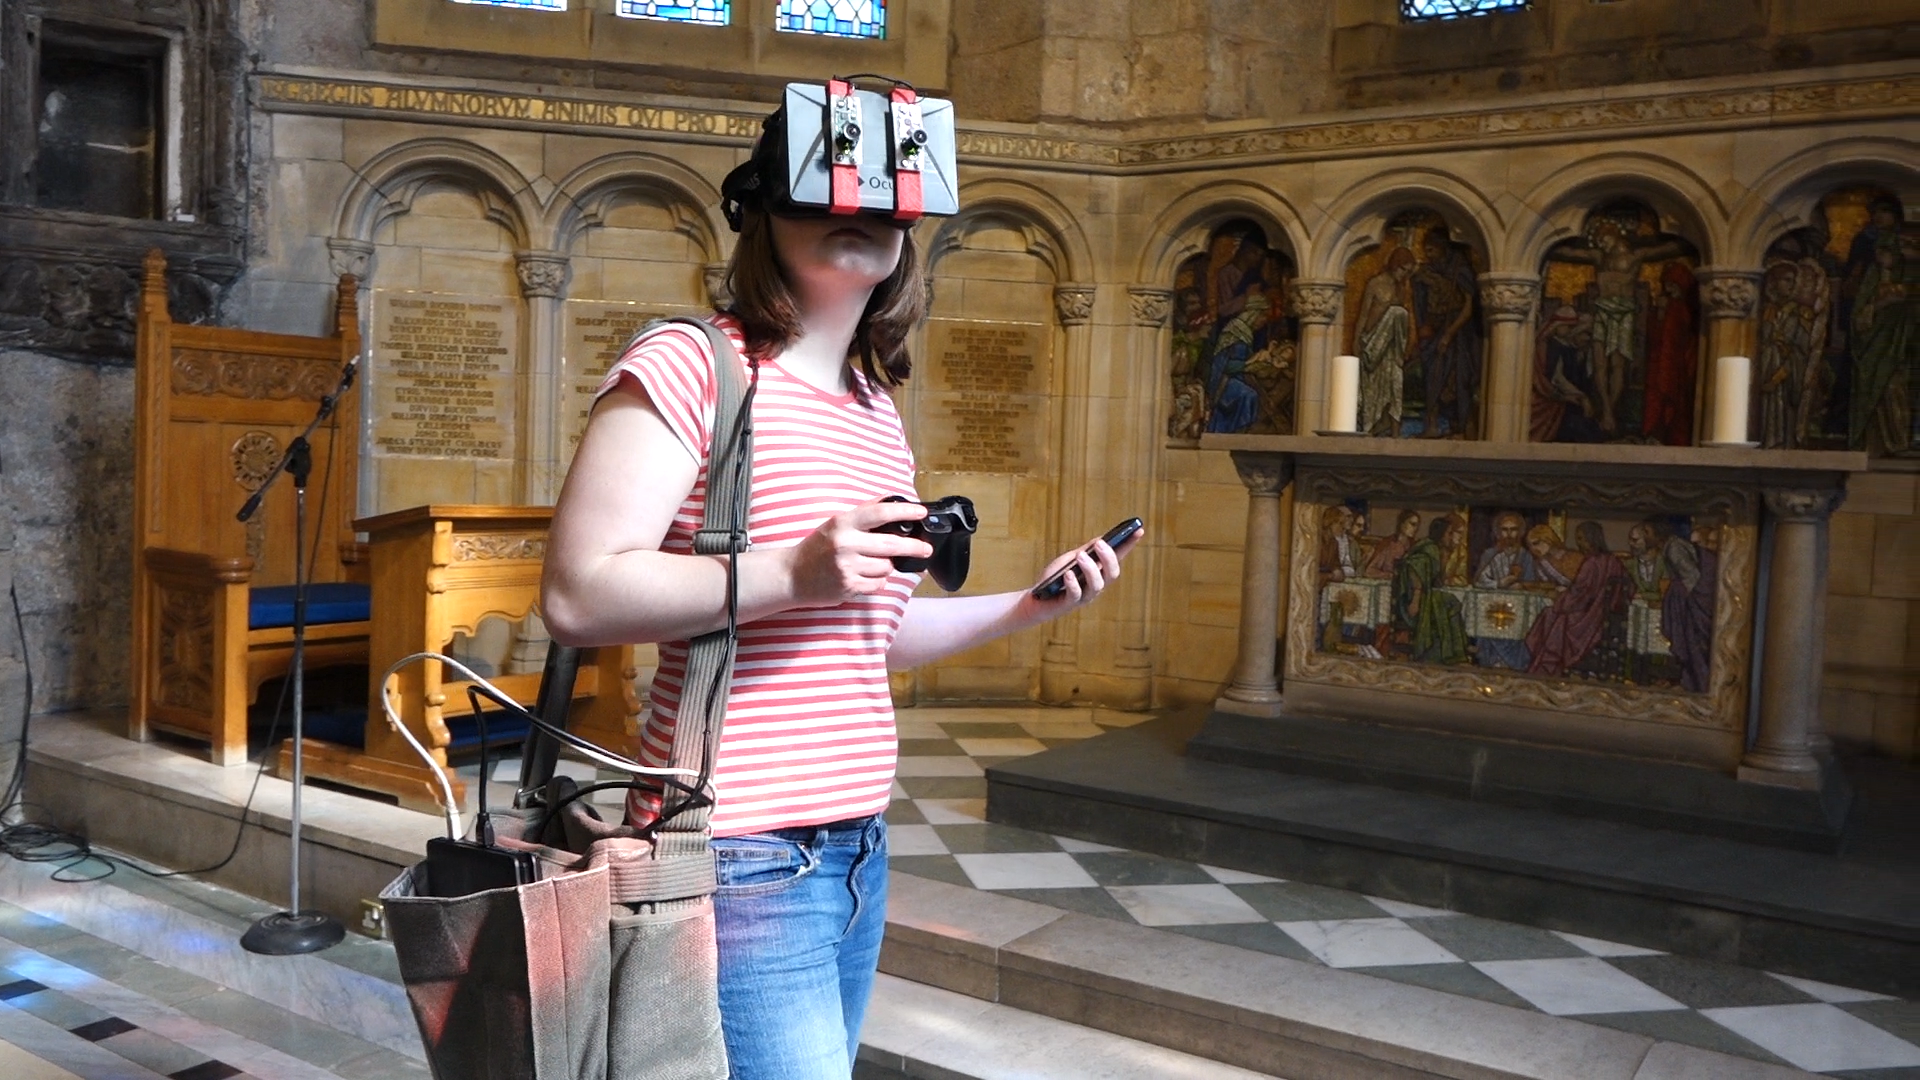
\includegraphics[width=\linewidth]{participant-f.png}
		\caption{Participant using Mirrorshades in a user study at St Salvator's chapel.}
		\label{participant-f.png}
	\end{center}
\end{figure}

\begin{figure}[ht]
	\begin{center}
		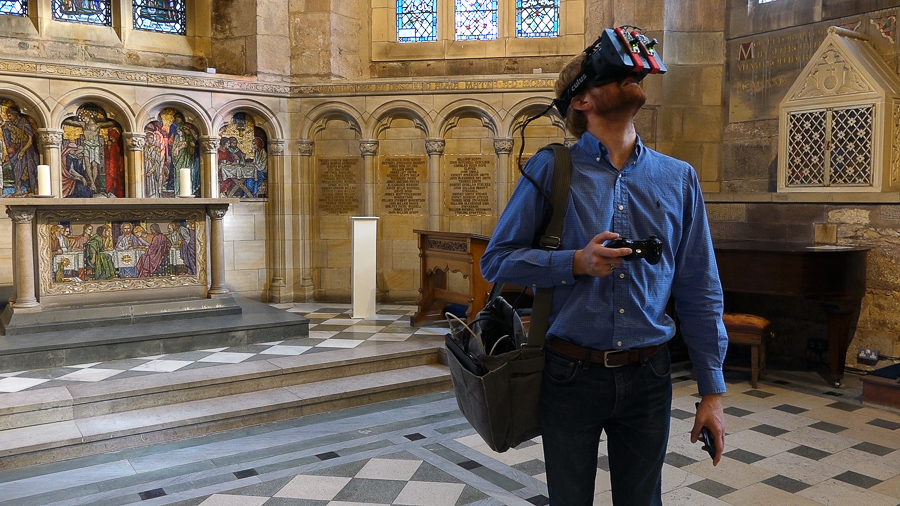
\includegraphics[width=\linewidth]{participant-m.png}
		\caption{Participant using Mirrorshades in a user study at St Salvator's chapel.}
		\label{participant-m.png}
	\end{center}
\end{figure}

%=========================================================================================================

\section{Stage 1 - PR for Virtual Heritage}

Previously when VR has been employed in virtual heritage scenarios, it has predominantly been implemented as CAVE experiences~\cite{Roussou2002}. Visitors to a museum or visitor centre will be offered the opportunity to step into a CAVE, possibly donning shutter glasses or similar apparatus to enable a stereoscopic 3D effect, to experience a VR reconstruction of a location, its contents \& actors. Some of these CAVE installations have featured physical control interfaces such as joystick \& 3D mouse~\cite{cabral:x3dexperience} \& haptic interfaces~\cite{Christou2006}, while others have tracked user movement, whether head only or full body  gestures (such as in figure \ref{VTTP_projection.png}). In common among these CAVE experiences is the fact that the VR content they present is experienced with a disconnect to the RW site that it pertains to, as the CAVE itself immerses users in VR visuals \& does not permit them to see any of their RW surroundings, comparable to the experience of weareing a VR HMD without see-through video functionality. Furthermore, the physical size of the CAVE limits the amount in any particular direction that a user can physically move, even if movement is encouraged due to its use as a control methodology.

With the promise of high performance VR HMDs at a consumer price point on the horizon, thanks largely to the rejuvenation in the field effected by Oculus, their use at cultural heritage sites for achieving similar experiences to previous CAVE installations is becoming more plausible \& brings with it certain benefits such as a reduction in the physical space required at the site for the installation. The OVW group's experience with presenting both experts \& interested amateurs, young \& old, with virtual heritage content via Oculus HMDs (both DK1 \& DK2, see section \ref{virtual-heritage-at-st-andrews}) has been very promising. These interactions have taken place in scenarios similar to those of existing CAVE scenarios; the user remains physically stationary \& uses a controller or gestures to move their virtual presence throughout the VR environment, whilst unable to observe their RW environment due to the nature of the HMD isolating them from RW visual stimuli.

In this first stage of the evaluation a comparison is made of this `traditional' style of interacting with VR content at a cultural heritage site wherein VR is experienced in isolation from RW, with both temporal \& spatial separation, against the `new' style afforded by the Mirrorshades platform, in which VR can be experienced in tandem with RW by allowing the user to move around their RW environment \& transition at any time into seeing the VR environment from the equivalent vantage point. Participants in this stage of the evaluation thus complete two scenarios wherein they interact with the RW St Salvator's chapel \& its corresponding VR reconstruction;

\begin{enumerate}
	\item \textbf{Traditional scenario} - Participants experience the RW \& VR chapels separately. They navigate the VR chapel from a stationary position, as VR has traditionally been employed at cultural heritage sites via CAVE installations \& by the OVW group with Oculus HMDs, using the Xbox controller to move around the VR environment observed via the DK1, with the DK1 obscuring their view of the RW chapel around them. Subsequently, they navigate the RW chapel without the DK1 or any associated equipment.
	\item \textbf{PR scenario} - Participants experience the RW \& VR chapels in tandem using the Mirrorshades platform. They wear the DK1, holding the Xbox controller in their right hand \& the smartphone in their left, with the laptop \& control box bundle in a satchel worn over one shoulder. Pressing a button on the Xbox controller triggers a transition between RW \& VR visual stimuli being displayed by the DK1.
\end{enumerate}

%=========================================================================================================

\subsection{Design of the Scenarios}

The scenarios were intended to mimic the style of exploration \& interaction that visitors to the chapel display, after observing the behaviour of such visitors on several occasions. From these observations, a common pattern of behaviour emerged: visitors enter the chapel from the North/West corner then proceed to walk Eastwards along the nave, pausing to look around after passing through the rood screen, before continuing along the nave toward the altar. They then pause in front of the alter upon reaching the end of the pews \& then walk North toward the tomb where they pause again to inspect it. Participants in this first stage of the evaluation process were instructed to imagine that they were performing a similar visit to the chapel \& to follow a similar path, pausing after the rood screen, at the end of the pews \& in front of the tomb to look around their environment(s) in more detail, however they were encouraged to stop \& look around at any times/positions that they wished \& not to feel restricted to the specific path \& locations. The intent of the scenario was to encourage a natural style of exploration despite the unusual situation of making use of bulky VR hardware, rather than to restrict them to an `on rails' experience. Participants were shown the map included as figure \ref{chapel-path} (North upwards) to help visualise the instructions.

\begin{figure}[h]
	\begin{center}
		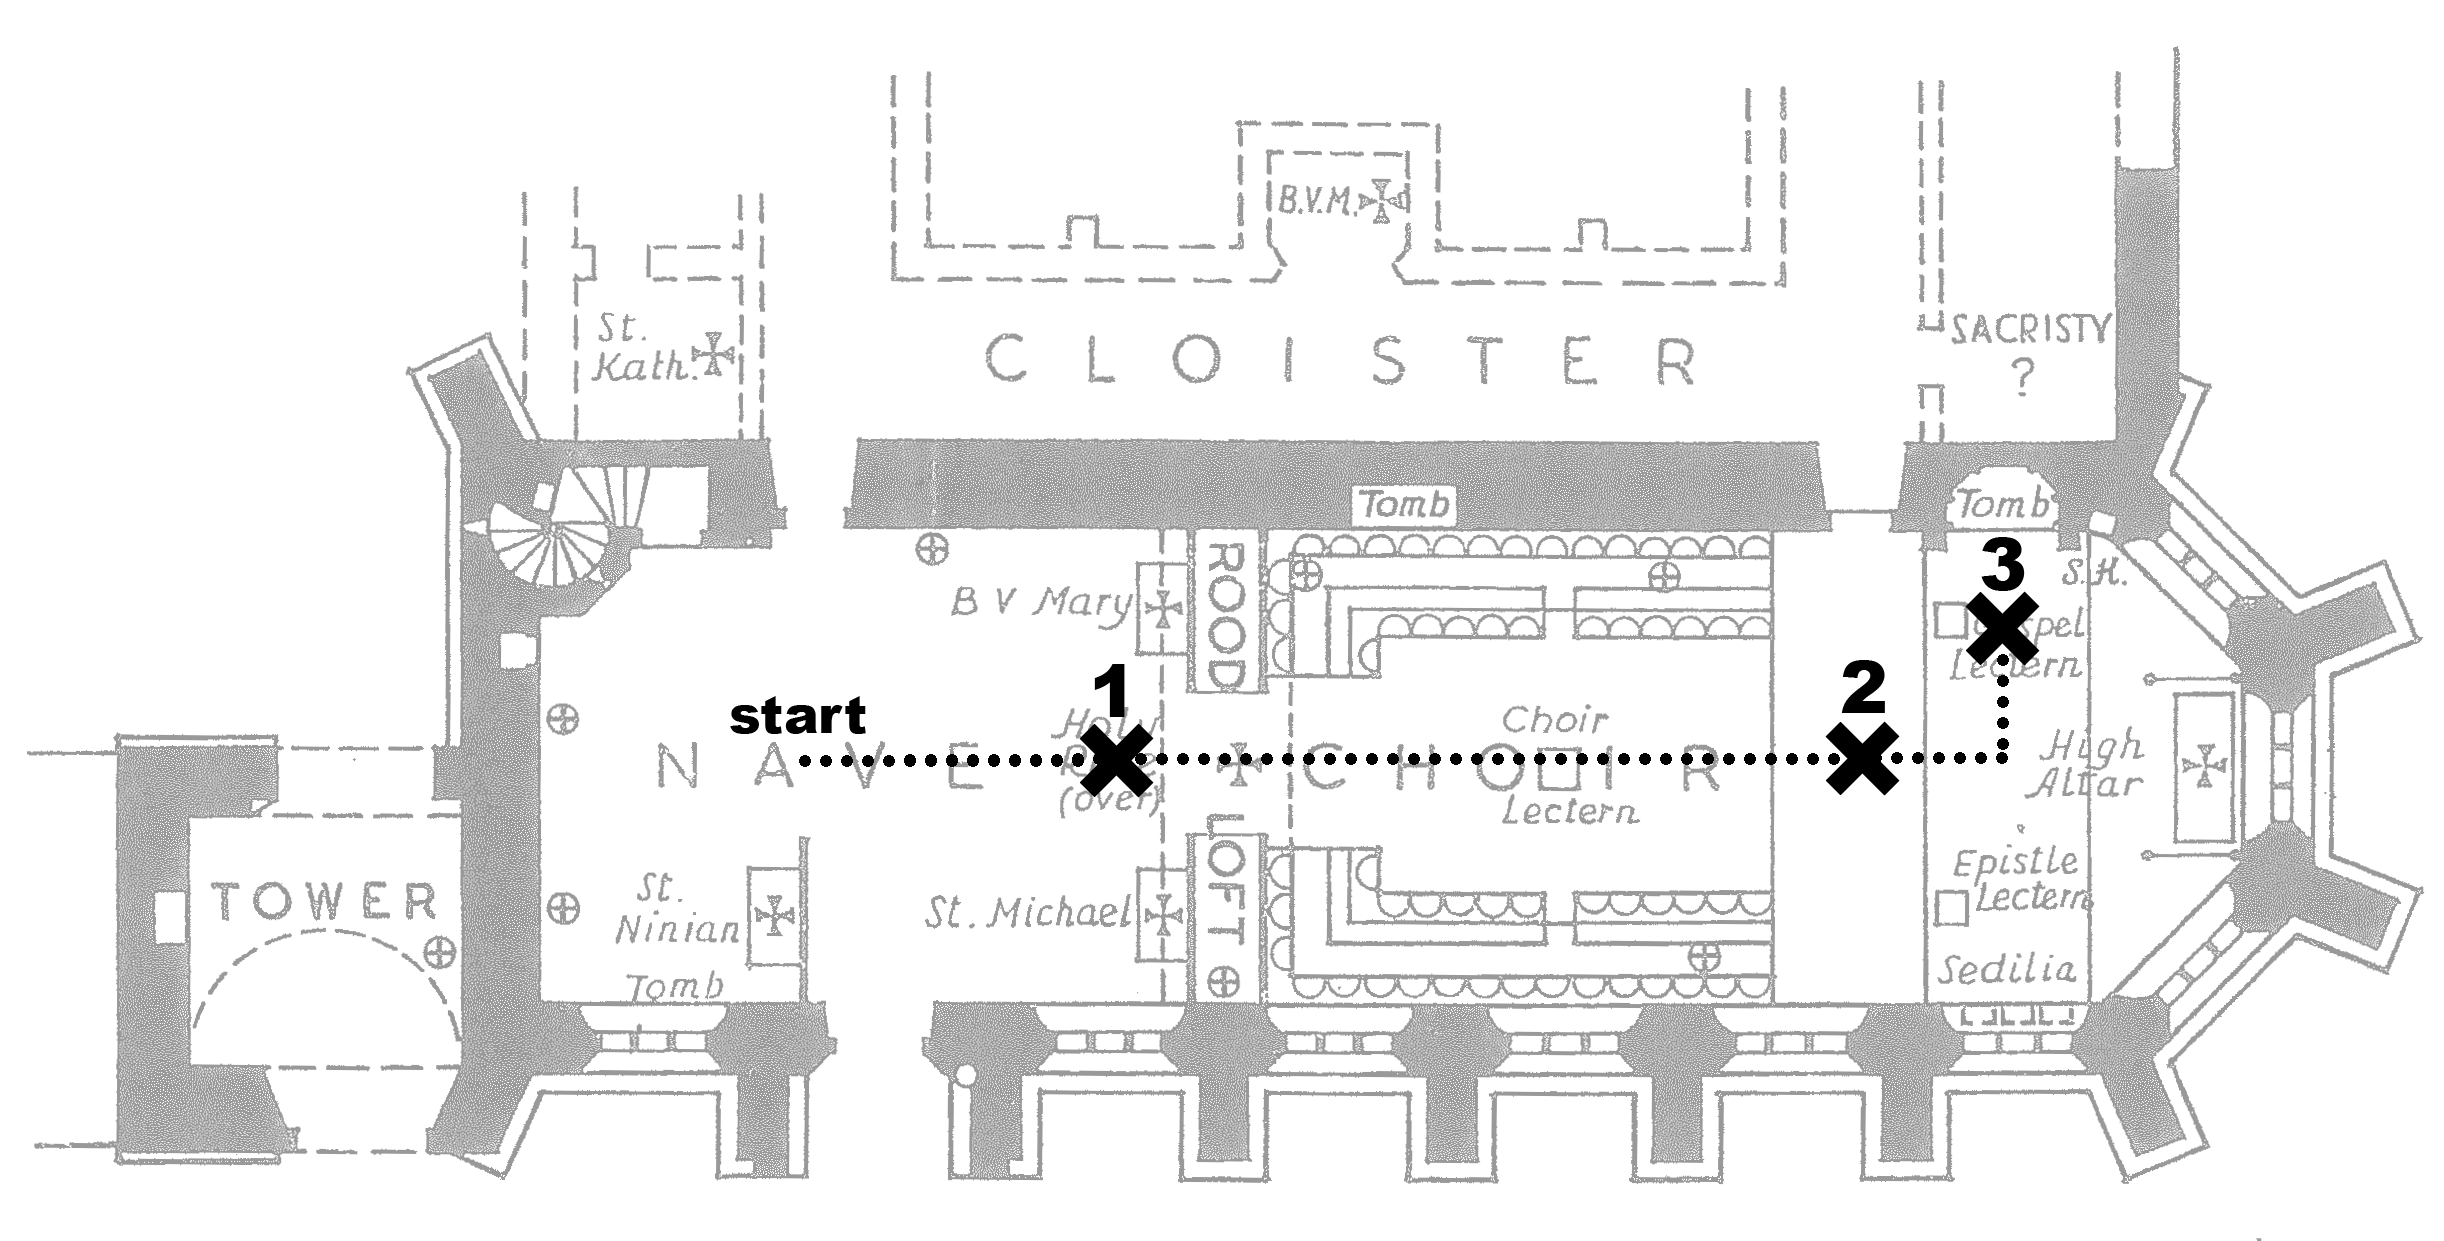
\includegraphics[width=.6\linewidth]{chapel-path.png}
		\caption{The path \& positions within the chapel that participants are instructed to attend to.}
		\label{chapel-path}
	\end{center}
\end{figure}

In the traditional scenario, participants interacted with the VR chapel using the DK1 \& Xbox controller, whilst seated. After completing the path in the VR chapel, they removed the DK1 \& walked the same path in the RW chapel. This behaviour alludes to how VR has previously been applied to cultural heritage sites such as St Salvator's chapel, wherein visitors would have the opportunity to experience a CAVE or stationary HMD based reconstruction of the site either before or after having explored the RW site. In the PR scenario, participants wore the DK1, held the Xbox controller in their right hand \& the smartphone in their left, with the laptop \& control box bundle in a satchel worn over a shoulder. They then walked the same path, but this time with the ability to transition at any time between viewing the RW chapel \& the VR chapel from the same vantage point.

In the PR scenario, participants had access to a single transition style, the transition with linear interpolation (section \ref{transition-with-linear-interpolation}), triggered by pressing \& holding the \texttt{A} button on the Xbox controller. As mentioned in section \ref{initial-testing}, this transition emerged as the `favourite' during initial tests within the OVW group. As such, it was chosen as the only transition style for the PR scenario in this first stage of evaluation wherein the focus of the investigation was upon comparing the PR scenario to the traditional scenario experience \& not upon gleaning details of the merits \& drawbacks exhibited by different PR implementations. The default view on the DK1's screen was 100\% RW with the transition causing a change to 100\% VR, a situation visualised upon the combined model in figure \ref{focus-locus-sensus-with-virtuality-continuum-with-transition}.

Before taking part in the two scenarios, participants were given the opportunity to familiarise themselves with the DK1 by spending a few minutes interacting with Oculus' `Tuscany' demo\footnote{\url{https://share.oculus.com/app/oculus-tuscany-demo}}. This demo was developed by Oculus themselves \& is distributed with the Rift Unity integration package. It represented at the time a very polished \& stable DK1 experience, ideal for introducing inexperienced users to HMD based VR. It was thus used to give participants an opportunity to acclimatize to the Rift, in order to reduce skewing their subsequent experiences with the St Salvator's chapel model due to drastically different levels of familiarity with the DK1 between the two scenarios.

%=========================================================================================================

\subsection{Evaluation Techniques}

The comparison of the traditional scenario against the PR scenario included collection of a variety of both qualitative \& quantitative data. All participants completed a pre-task questionnaire which provided calibration for latter data by enquiring about age, gender identity, previous experience with VR HMDs \& whether they had previously visited St Salvtor's chapel, both RW \& VR (the RW chapel is open to the public \& a version of the VR reconstruction is publicly accessible via the OVW group's OpenSim grid). The System Usability Scale (SUS)~\cite{Brooke1996} was used to provide a basic comparison between the usability of the two scenarios, while a 12-item Likert-type questionnaire was used to collect opinions on more specific aspects of the experience of both scenarios. At the end of the session, participants were engaged in a short structured interview in order to allow them to elaborate upon their experience in a more free form manner. Finally, in addition to the DK1 visuals being recorded via ShadowPlay, log data was collected during both scenarios, capturing the following information to a tab separated variable (\texttt{.tsv}) file for each frame rendered to the DK1's screen;

\begin{center}
\begin{longtable}{| l | p{8cm} |}

\hline

\textbf{Field} & \textbf{Description} \\

\hline

\texttt{<frame number>} & Incremented with each frame pushed to the DK1, starting at 0 when the Unity application is fun. \\

\hline

\texttt{<timestamp>} & According to the laptop's internal clock. \\

\hline

\texttt{<original\_position>} & The position as a Unity \texttt{Vector3} where the participant begins the experiment (as reported by IndoorAtlas). \\

\hline

\texttt{<position>} & The position as a Unity \texttt{Vector3} where the participant is on this frame (as reported by IndoorAtlas). \\

\hline

\texttt{<delta\_x>} \& \texttt{<delta\_z>} & The difference in the \texttt{x} \& \texttt{z} axes between \texttt{<original\_position>} \& \texttt{<position>} on this frame. Change in elevation (\texttt{y} axis) is not recorded, as IndoorAtlas does not provide elevation data \& the area of St Salvator's chapel used throughout the studies is largely level. \\

\hline

\texttt{<left\_rotation>} \& \texttt{<right\_rotation>} & The orientations as Unity \texttt{Quaternion} of the two Unity camera game objects. The orientation of these Unity objects is tied to the orientation of the DK1, so these values represent the orientation of the participant's head on this particular frame. \\

\hline

\texttt{<base\_oapcity>} & The maximum opacity of the game objects upon which the camera feeds are rendered. This is how reduced maximum opacity (see section \ref{subsub-baseopacity}) is implemented. \\

\hline

\texttt{<left\_opacity>} \& \texttt{<right\_opacity>} & The opacity on this frame of the game objects upon which the camera feeds are rendered. \\

\hline

\texttt{<auto\_tick>} & Whether a periodic switch is in progress (see section \ref{subsub-periodic}). \\

\hline

\texttt{<auto\_duration>} \& \texttt{<auto\_spacing>} & The interval \& duration values of the periodic hard switching (if applicable). \\

\hline

\texttt{<framerate>} & An estimate of the current frame rate (frames per second). \\

\hline

\texttt{<A\_button>}, \texttt{<B\_button>} \& \texttt{<right\_trigger>} & The current values of these inputs on the Xbox controller. For the \texttt{A} \& \texttt{B} buttons this is binary, either pressed or not, while for the trigger it is a numeric value representing the amount that the trigger is being depressed. \\

\hline

\end{longtable}
\end{center}

%=========================================================================================================

%\subsection{Process}

%The stage 1 investigations took place as follows;

%\begin{enumerate}
%	\item Participants completed the pre-task questionnaire.
	
%	\item Participants were given the opportunity to familiarise themselves with the DK1 by spending a few minutes interacting with Oculus' `Tuscany' demo\footnote{\url{https://share.oculus.com/app/oculus-tuscany-demo}}. This demo was developed by Oculus themselves \& is distributed with the Rift Unity integration package. It represented at the time a very polished \& stable DK1 experience, ideal for introducing inexperienced users to HMD based VR. It was thus used to give participants an opportunity to acclimatize to the Rift, in order to reduce skewing their subsequent experiences with the St Salvator's chapel model due to drastically different levels of familiarity with the DK1 between the two scenarios.
	
%	\item Participants completed the traditional scenario.
	
%	\item Participants completed the SUS questionnaire \& the 12-item Likert-type questionnaire for their experience with the traditional scenario.
	
%	\item Participants completed the PR scenario.
	
%	\item Participants completed the SUS questionnaire \& the 12-item Likert-type questionnaire for the PR scenario.
	
%	\item Participants are engaged in a short structured interview.
%\end{enumerate}

%=========================================================================================================

\section{Hypotheses}

This first stage of evaluation was designed to ascertain whether applying mobile PR to a cultural heritage scenario results in an improvement in participant engagement with \& understanding of the relationships between the RW \& VR environments, compared to a traditional virtual heritage scenario, by addressing the problems of spatial \& temporal separation inherent with the traditional scenario by imparting upon the participant the ability to transition at will between equivalent vantage points within the RW \& VR environments.

Participants were expected to report that the PR scenario did allow them to better compare \& contrast the RW \& VR environments, identify differences between the RW \& VR environments \& gain a better understanding of how the RW \& VR environments relate to each other. However it was also expected that some participants would report that having to `split' their attention between the two environments in the PR scenario led to lessened engagement \& understanding \& that the visual quality of the RW view through the cameras led to them preferring the traditional scenario.

It was expected that the cumbersome nature of the PR scenario in terms of the hardware that needed to be carried by the participant \& the reduced quality of viewing the RW environment via the cameras would have a noticeable effect upon participants' movement (both position \& head orientation) in the PR scenario, most likely a restriction.

SUS scores for the PR scenario were expected to average lower than those for the traditional scenario, due to the cumbersome nature of the platform when performing the mobile scenario; during the stationary scenario, participants are seated, whilst during the mobile scenario they are required to carry a satchel over one shoulder \& hold a smartphone in their left hand. Participants who were able to overcome this cumbersomeness were expected to respond more favourably to the mobile scenario than those who could not.

The 12-item Likert-type questionnaire was expected to reveal several distinctions. In particular;
\begin{itemize}
	\item Participants will find it easier to compare \& contrast RW \& VR environments in the PR scenario than in the traditional scenario (q2)
	\item Participants will experience a greater  sense of `being in' the VR environment in the PR scenario than in the traditional scenario, due to physical movement/embodiment~\cite{Groten2011} (q4)
	\begin{itemize}
		\item Furthermore, participants will have a greater sense of `being in the past' in the PR scenario than in the traditional scenario (q7)
	\end{itemize}
	\item Participants will maintain greater awareness of both RW \& VR environments in the PR scenario than in the traditional scenario (q5)
	\item Participants will notice more differences between RW \& VR environments in the PR scenario than in the traditional scenario (q10)	
	\item Participants will gain a better understanding of what the chapel was like in the past in the PR scenario than in the traditional scenario (q12)
\end{itemize}

In addition to substantiating or refuting questionnaire results \& interview responses, the log data themselves were expected to provide insight into relationships between several aspects of the traditional \& PR scenarios, such as;
\begin{itemize}
	\item Head movement (pitch \& yaw) will be more restricted in the PR scenario compared to the traditional scenario
	\item Participants will display an aversion to looking around (even at RW) when moving in the mobile scenario
	\item Head movements will be larger discrete changes in the traditional scenario compared to the PR scenario
	\item Tendency to only look at VR when looking around
\end{itemize}

Interview transcripts were expected to lend support to the following assumptions;
\begin{itemize}
	\item the PR scenario makes it easier to spot differences between RW \& VR than the traditional scenario
	\item the PR scenario reveals differences that the traditional scenario didn't
	\item the traditional scenario does not reveal differences that the PR scenario didn't
	\item the PR scenario is preferred \& is user-reported as 'more engaging' than the traditional scenario
\end{itemize}

Assessing the severity of the issues raised by this first stage of investigation is important such that future PR implementations can be informed to allow them to achieve a quality of experience where participants do not feel that the drawbacks outweigh the benefits, such as feeling restricted from performing transitions due to the jarring nature of them or preferring a traditional scenario compared to a PR scenario because the visual acuity of seeing the RW unmediated compared to mediated via a video see-through HMD is so much better that the immediacy of comparison between RW \& VR afforded by the PR scenario is not a big enough incentive.

%=========================================================================================================

\section{Stage 1 Results}

A total of 6 participants completed the stage 1 investigation;
\begin{itemize}
	\item Age ranged from 21 to 26, with a mean of 23.3 \& a standard deviation of 1.86
	\item 3x identified as male \& 3x as female
	\item All reported previous experience with a games console controller
	\item 1x reported previous experience with a HMD
	\item 2x reported having previously visited the chapel
	\item None had previously experienced the virtual chapel
\end{itemize}

%=========================================================================================================

\subsection{SUS}
As expected, the PR scenario scored lower on SUS than the traditional scenario (see figure \ref{sus.png}).

\TwoFig{1/sus.png}{SUS results.}{sus.png}
       {1/post_task_questionnaire_boxplot.png}{12-item questionnaire results.}{post_task_questionnaire_boxplot.png}

%=========================================================================================================

\subsection{Likert-type Questionnaires}

One participant did not complete the Likert-type questionnaires. This was the only participant to report previous experience with a HMD.

When considering the responses to the questionnaires (see figure \ref{post_task_questionnaire_boxplot.png}), remembering that the participant who reported previous HMD experience is not represented, several observations can be made.

\begin{itemize}
	\item Participants enjoyed the PR scenario more than the traditional scenario (q1)
	\item Participants found it easier to compare features from past \& present in the PR scenario (q2)
	\item Perceived motion sickness/dizziness was not noticeably different between the two scenarios (q3)
	\item There was a greater ‘sense of presence’ in the VR environment in the PR scenario (q4)
	\item There was a greater awareness of both environments in the PR scenario (q5)
	\item Participants found the PR scenario a more rewarding way to explore the chapel (q6)
	\item Participants had a greater sense of being in the past in the PR scenario (q7)
	\item Both scenarios scored fairly low for participants thinking they would have preferred a conventional monitor (q8)
	\item The PR scenario further changed participants’ understanding of the chapel than the traditional scenario (q9)
	\item Both scenarios scored equally low for participants’ thinking they did not notice differences between RW \& VR (q10)
	\item The visual quality of the headset was perceived as being worse in the mobile scenario (q11). Whilst the visual quality of the VR visuals was identical in both scenarios, this result is presumably because during the PR scenario the participants were viewing the RW environment upon the DK1's screen via the cameras, with much lower visual acuity than in the traditional scenario where they observed the RW environment unmediated.
	\item Participants felt that they better understood what the chapel was like in the past after the PR scenario, compared to the traditional scenario (q12)
\end{itemize}

It is worth highlighting that although the PR scenario scored lower in SUS than the traditional scenario, both scenarios scored highly in question 2 \& lowly in question 8 of the Likert-type questionnaires.

%=========================================================================================================

\subsection{Interview Transcripts}

Studying the structured interviews that took place after participants had completed both scenarios (interviews were recorded \& later transcribed) provided a wealth of qualitative feedback about the stage 1 investigation.

All participants said that the PR scenario was (much) more engaging than the traditional scenario, even though 2x participants said that they preferred the seated scenario. Of those that said they preferred the traditional scenario, one did not find it comfortable to walk with the headset \& the other said that they got a better understanding of the past when sat down wearing the DK1. The participant who found it uncomfortable to walk with the headset was notably taller than all of the other participants in this stage. This is worth mentioning as the `height' of the virtual cameras in the VR reconstruction was fixed with reference to the UK average height of 5 feet 9 inches \& was not changed to account for different participant heights, as this would have required a lengthy calibration phase for each \& every participant). Thus for a participant of average height, the discrepancy between their RW viewpoint \& their VR viewpoint was minimal, however for a particularly short or tall participant this discrepancy would have been much worse \& may have contributed to the discomfort of walking with the DK1 as each transition between RW \& VR would have resulted in a perceptible shift in height. Those that said that the preferred the PR scenario alluded to the immediacy of comparison between RW \& VR afforded by it as a contributing factor.

Twice as many participants reported that the PR scenario made it easier to spot differences between RW \& VR as reported that the traditional scenario made it easier. The quality of the cameras was mentioned as a possible detractor by one of the participants who answered that the traditional scenario made it easier, while again the immediacy of comparison possible between RW \& VR was alluded to in support of the PR scenario for spotting differences, with one participant directly mentioning then confirming this immediacy as the enabler of spotting more differences. One participant mentioned that with the traditional scenario it was not clear that you were \textit{``trying to look into the past''} but in the PR scenario it was obvious because \textit{``you can see the differences''}, while another participant directly said that s/he preferred the PR scenario because \textit{``it was easier to compare \& contrast between the real world \& the virtual one''}.

4 out of 6 participants reported noticing differences between RW \& VR in the PR scenario that they did not notice in the traditional scenario. In particular, the different position of the rood screen was mentioned by several participants \& one participant was able to list multiple differences that s/he had spotted in the PR scenario that they had not noticed in the traditional scenario.

The one participant to report experiencing motion sickness elaborated that it was worse when using the DK1 in the traditional scenario than when walking with the DK1 in the PR scenario, because \textit{``sitting down \& moving around feels weird} (a reference to moving throughout the VR environment using the Xbox controller whilst physically stationary sitting on a chair). This observation alludes to the idea of physical embodiment/movement improving a VR experience, by representing the opposite position of restricted movement \& lack of matching embodiment worsening the VR experience.

The accuracy \& lag of the indoor positioning was cited by one participant as needing work, because it \textit{``caught me off guard twice''}. Furthermore, the quality of the RW visuals when perceived through the DK1 \& cameras was mentioned by several participants as needing improvement, with one specifically mentioning that a higher \textit{``resolution''} was needed.

%=========================================================================================================

\subsection{Log Data}

For the traditional scenario log data was recorded while each participant was engaging with the VR chapel, in a seated position \& using the Xbox controller to navigate the VR environment. For the PR scenario log data was recorded throughout the whole scenario, such that data are available for both the periods in which participants were observing the RW chapel via the DK1 \& cameras in addition to the periods in which participants were observing the VR chapel. As such, several comparisons can be made between these data. Within the PR scenario, comparisons can be made between the periods that participants were observing RW \& the periods that participants were observing VR. Between the traditional scenario \& the PR scenario, comparisons can be made between the VR section of the traditional scenario \& the periods that participants were observing VR in the PR scenario. Log data was not captured for participant 2 \& was not captured for the traditional scenario for participant 5.

When looking at either scenario (the VR section of the traditional scenario \& both RW \& VR periods of the PR scenario) it is immediately obvious that participants looked to their sides \& turned their heads horizontally (yaw) far more than they looked above \& beneath themselves \& tilted their heads vertically (pitch). This relationship is shown in figures \ref{1_pitch_yaw_2up.png}, \ref{4_pitch_yaw_2up.png} \& \ref{6_pitch_yaw_2up.png}, which show pitch \& yaw plotted against time for both the traditional scenario \& the PR scenario, for participants 1, 4 \& 6 respectively.

\begin{figure}[]
	\begin{center}
	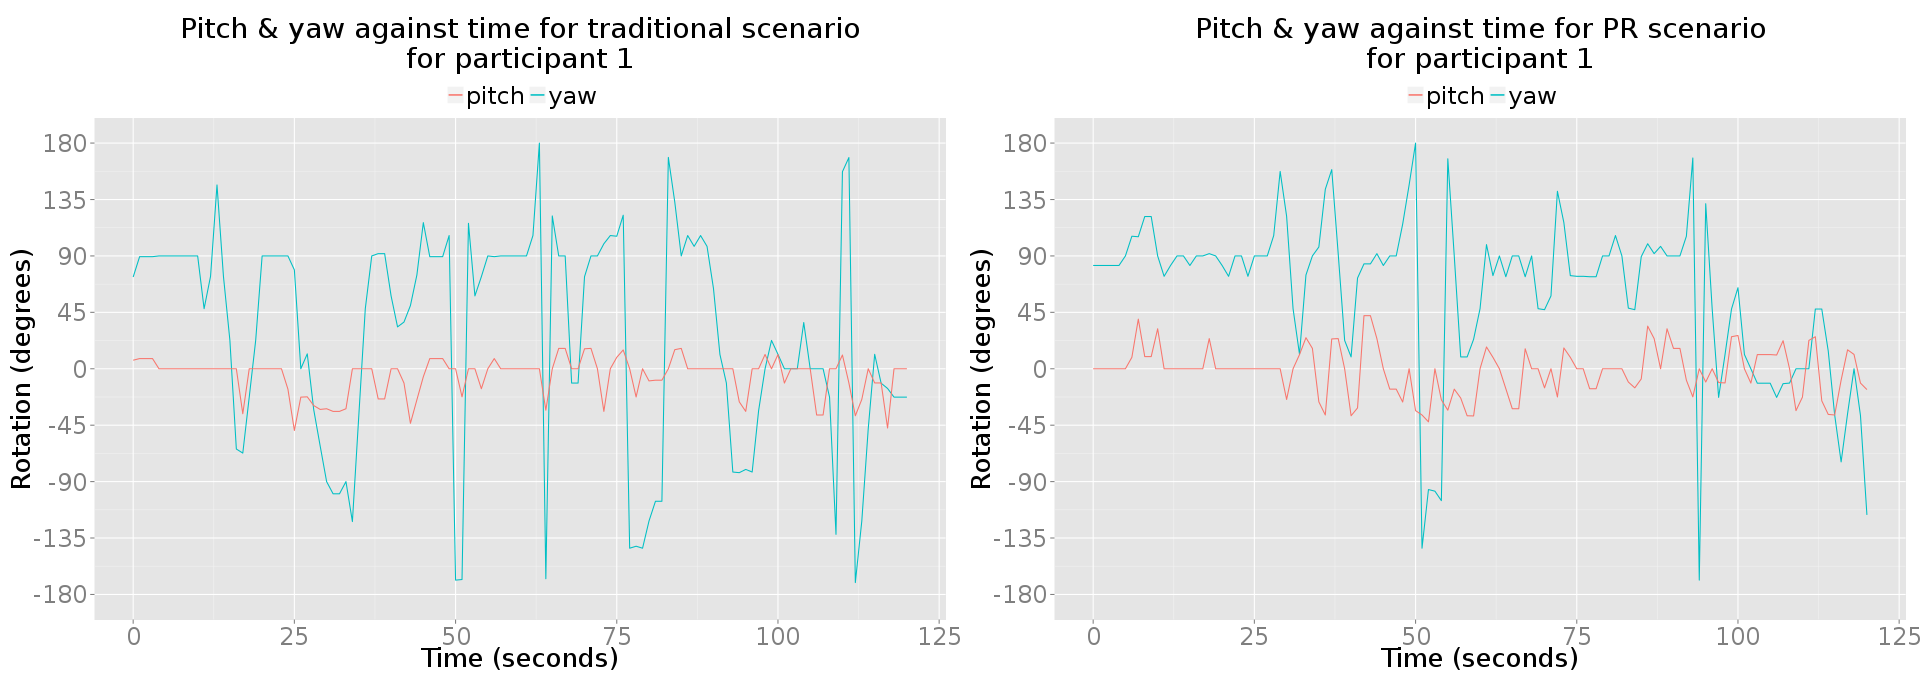
\includegraphics[width=\textwidth]{1/1_pitch_yaw_2up.png}
	\caption{Pitch \& yaw against time for participant 1 in traditional \& PR scenarios.}
	\label{1_pitch_yaw_2up.png}
	\end{center}
\end{figure}

\begin{figure}[]
	\begin{center}
	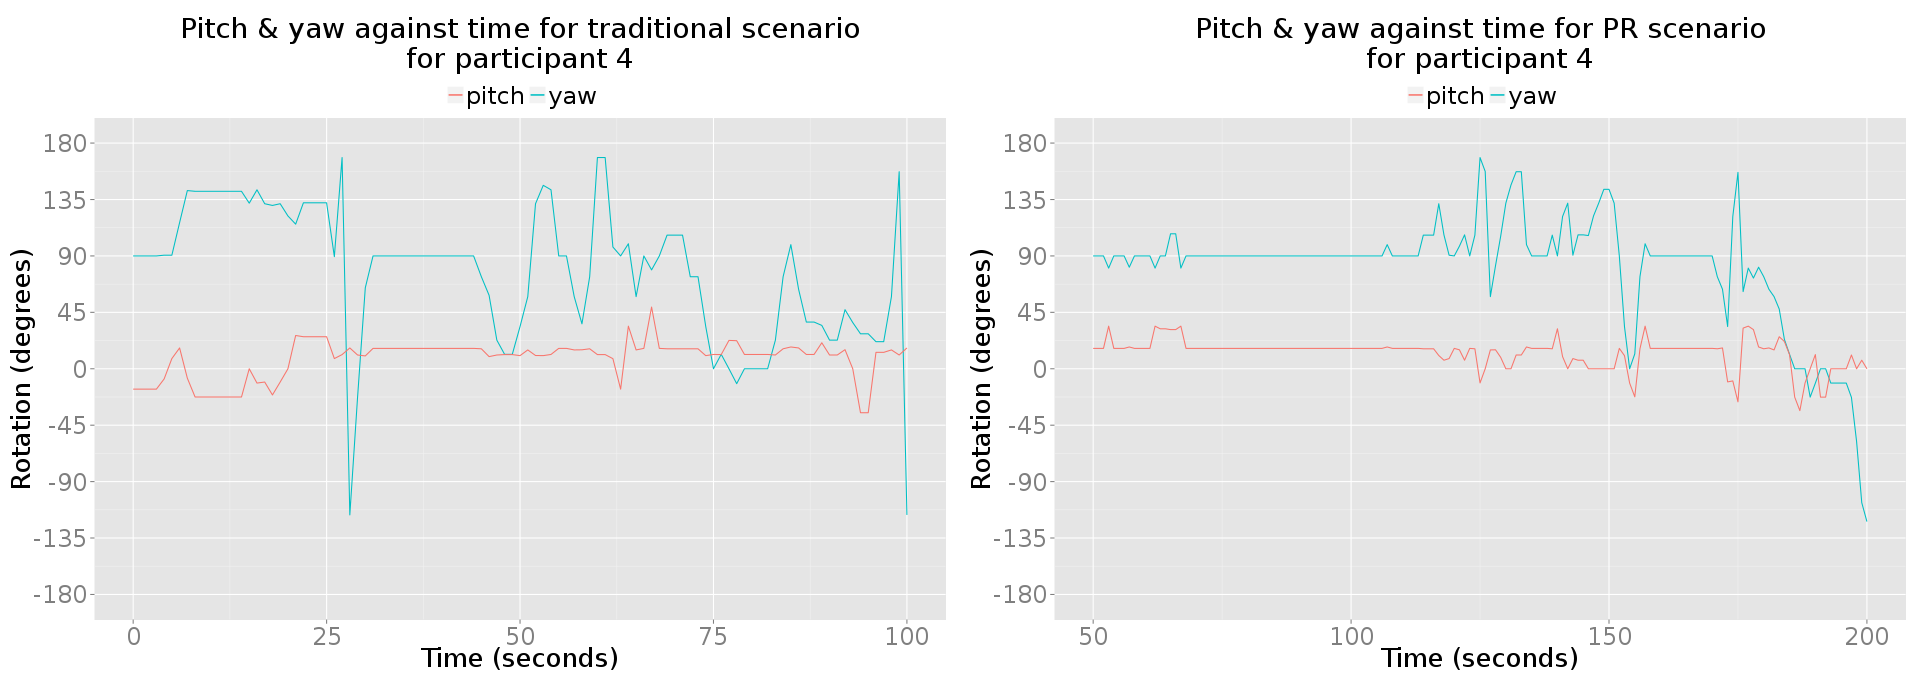
\includegraphics[width=\textwidth]{1/4_pitch_yaw_2up.png}
	\caption{Pitch \& yaw against time for participant 4 in traditional \& PR scenarios.}
	\label{4_pitch_yaw_2up.png}
	\end{center}
\end{figure}

\begin{figure}[]
	\begin{center}
	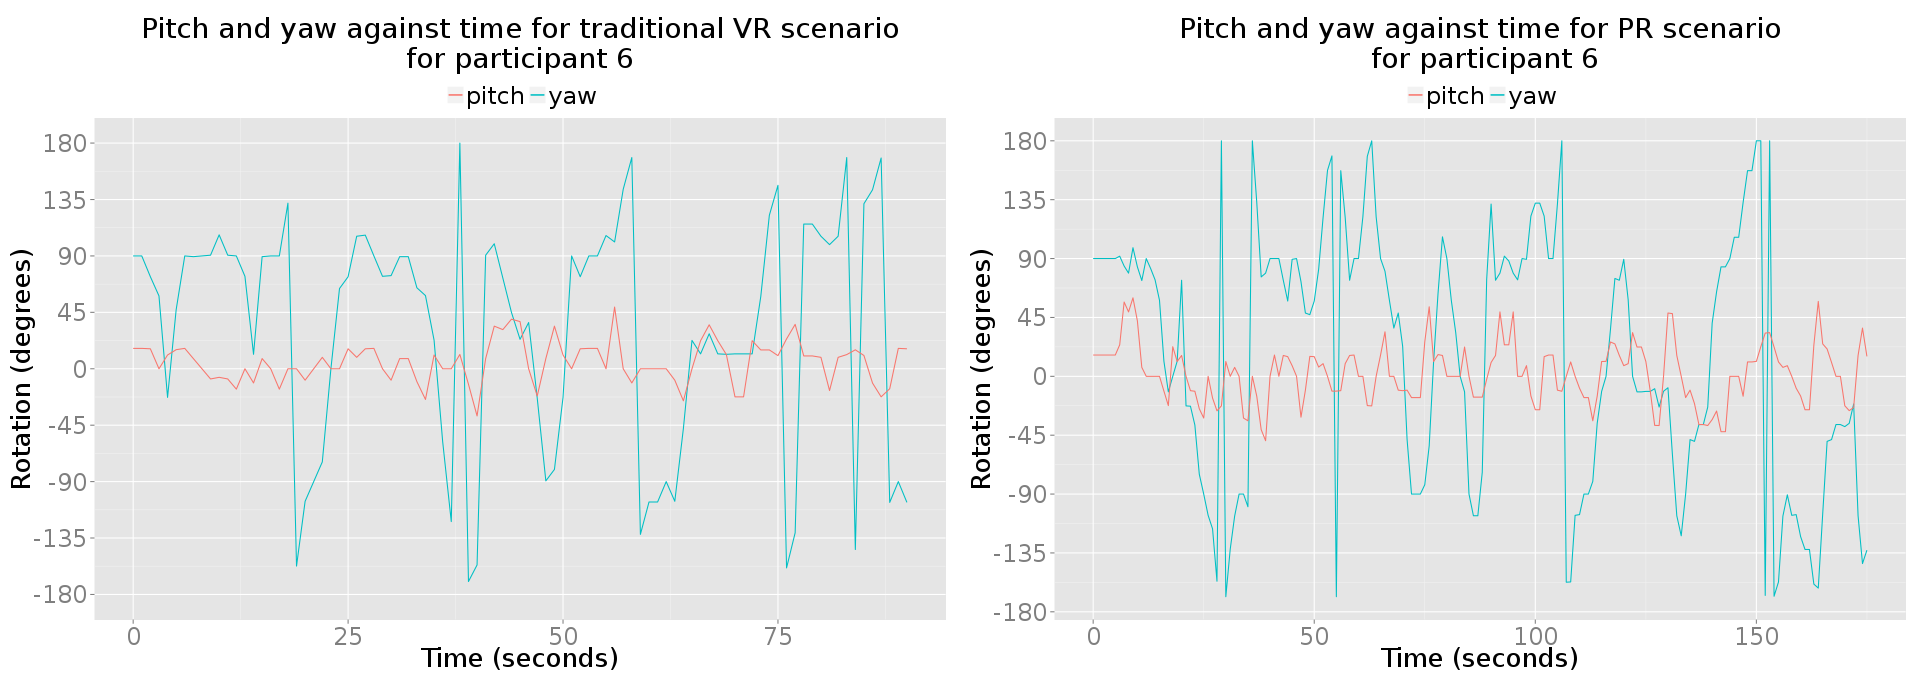
\includegraphics[width=\textwidth]{1/6_pitch_yaw_2up.png}
	\caption{Pitch \& yaw against time for participant 6 in traditional \& PR scenarios.}
	\label{6_pitch_yaw_2up.png}
	\end{center}
\end{figure}

The relationship is also evident when considering the standard deviation in pitch \& yaw across both scenarios, shown by table \ref{sdpitchyawtrad} for the traditional scenario \& table \ref{sdpitchyawpr} for the PR scenario.

\begin{table}
\begin{center}
\begin{minipage}[t]{.47\linewidth}
\begin{center}
\begin{tabular}{|c|c|c|}
\hline

\textbf{Participant} & \textbf{Pitch (\textdegree)} & \textbf{Yaw (\textdegree)} \\

\hline

1 & 14.977 & 86.211 \\

\hline

3 & 16.684 & 60.545 \\

\hline

4 & 10.516 & 53.805 \\

\hline

5 & no data & no data \\

\hline

6 & 16.172 & 92.416 \\

\hline
\end{tabular}
\caption{Standard deviation in pitch \& yaw for traditional scenario.}
\label{sdpitchyawtrad}
\end{center}
\end{minipage}
%
\begin{minipage}[t]{.47\linewidth}
\begin{center}
\begin{tabular}{|c|c|c|}
\hline

\textbf{Participant} & \textbf{Pitch (\textdegree)} & \textbf{Yaw (\textdegree)} \\

\hline

1 & 19.186 & 63.427 \\

\hline

3 & 24.228 & 51.666 \\

\hline

4 & 11.723 & 44.526 \\

\hline

5 & 16.542 & 39.601 \\

\hline

6 & 21.999 & 97.122 \\

\hline
\end{tabular}
\caption{Standard deviation in pitch \& yaw for PR scenario.}
\label{sdpitchyawpr}
\end{center}
\end{minipage}
\end{center}
\end{table}

When comparing pitch \& yaw data between the RW \& VR periods within the PR scenario, it is immediately noticeable that for some participants there was substantially more head movement in terms of pitch (vertical movement) \& yaw (horizontal movement) while they were perceiving VR stimuli than while they were perceiving RW stimuli. This is particularly evident when plotting these pitch \& yaw data against time with the RW/VR visuals indicated. Figure \ref{1_pitch_yaw.png} shows the pitch \& yaw data for participant 1, who prominently displayed this tendency toward greater head movement while viewing VR than RW. The coloured background of the plot indicates which environment the participant was perceiving; blue for RW \& green for VR.

\begin{figure}[h]
	\begin{center}
	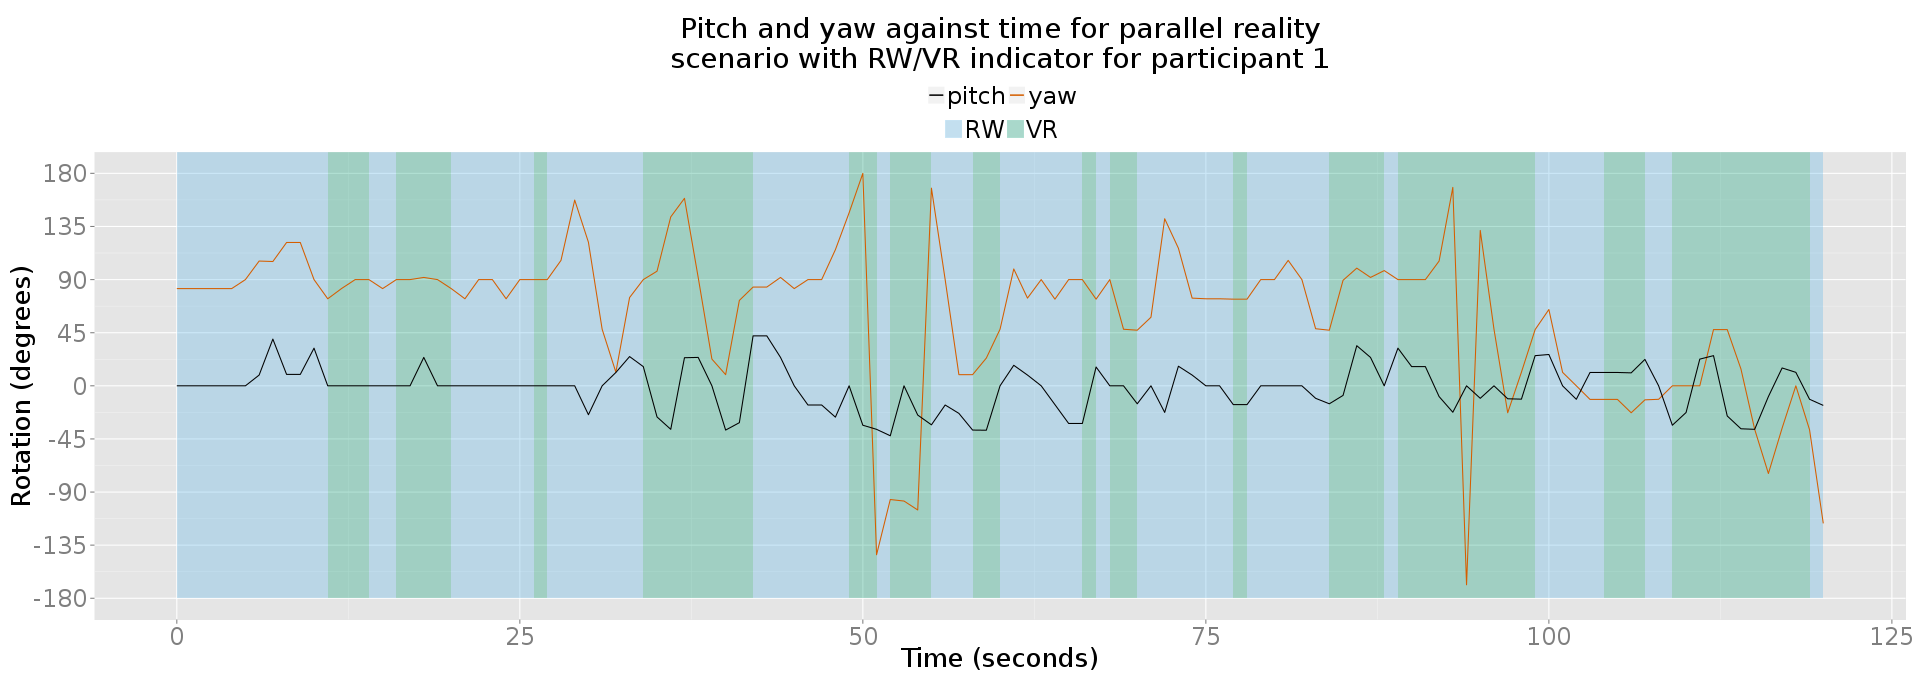
\includegraphics[width=\textwidth]{1/1_pitch_yaw.png}
	\caption{Pitch \& yaw against time for participant 1 in PR scenario.}
	\label{1_pitch_yaw.png}
	\end{center}
\end{figure}

As can be seen in figure \ref{3_pitch_yaw.png} this relationship is even more prevalent in the data from participant 3, while the data from participant 5 in figure \ref{5_pitch_yaw.png} shows the relationship to a lesser extent.

\begin{figure}[h]
	\begin{center}
	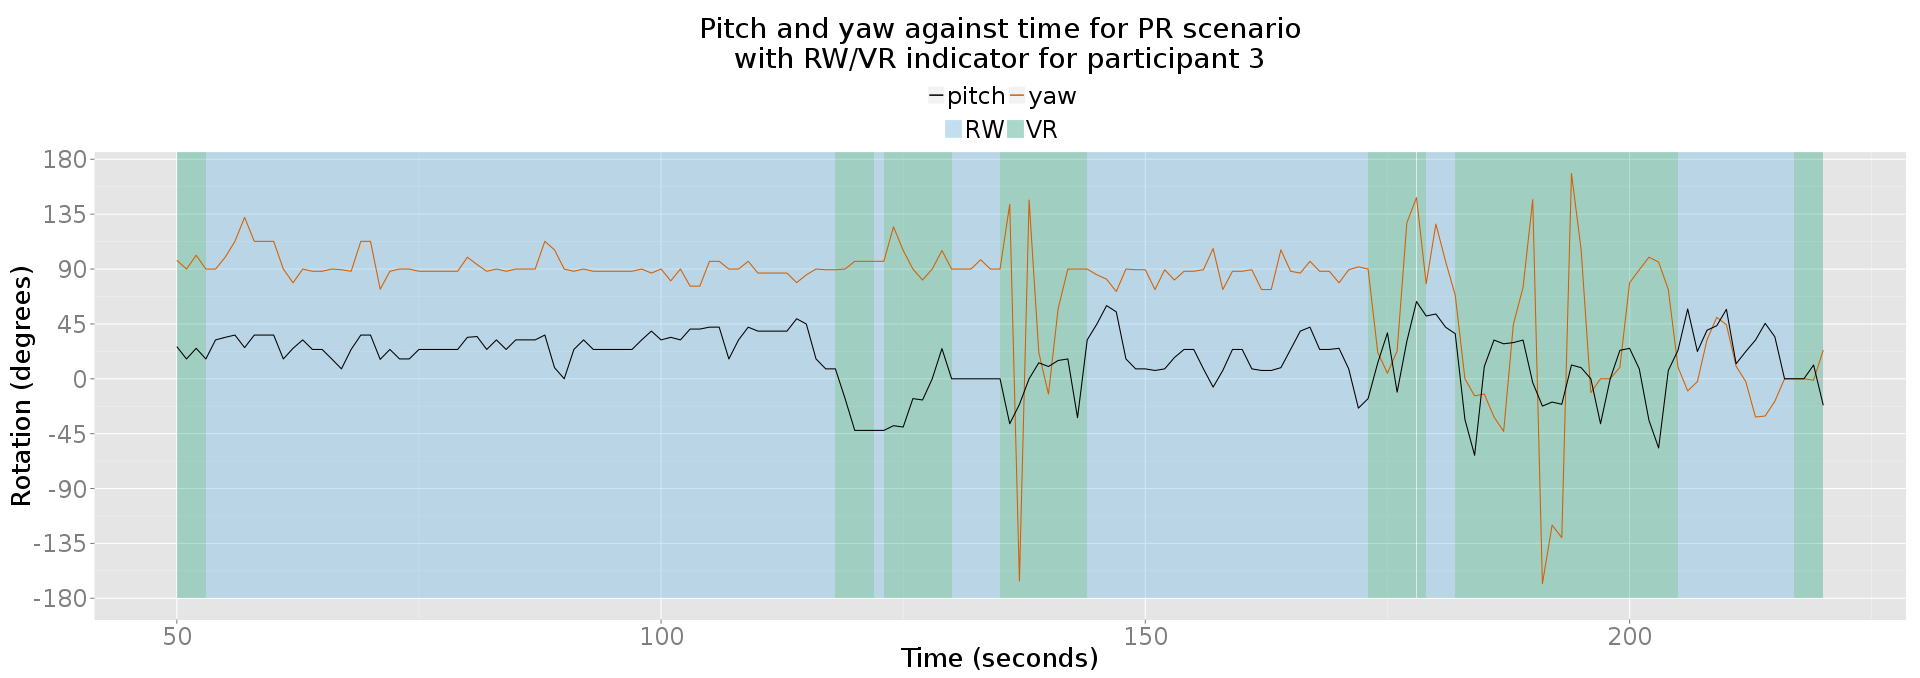
\includegraphics[width=\textwidth]{1/3_pitch_yaw.png}
	\caption{Pitch \& yaw against time for participant 3 in PR scenario.}
	\label{3_pitch_yaw.png}
	\end{center}
\end{figure}

\begin{figure}[h]
	\begin{center}
	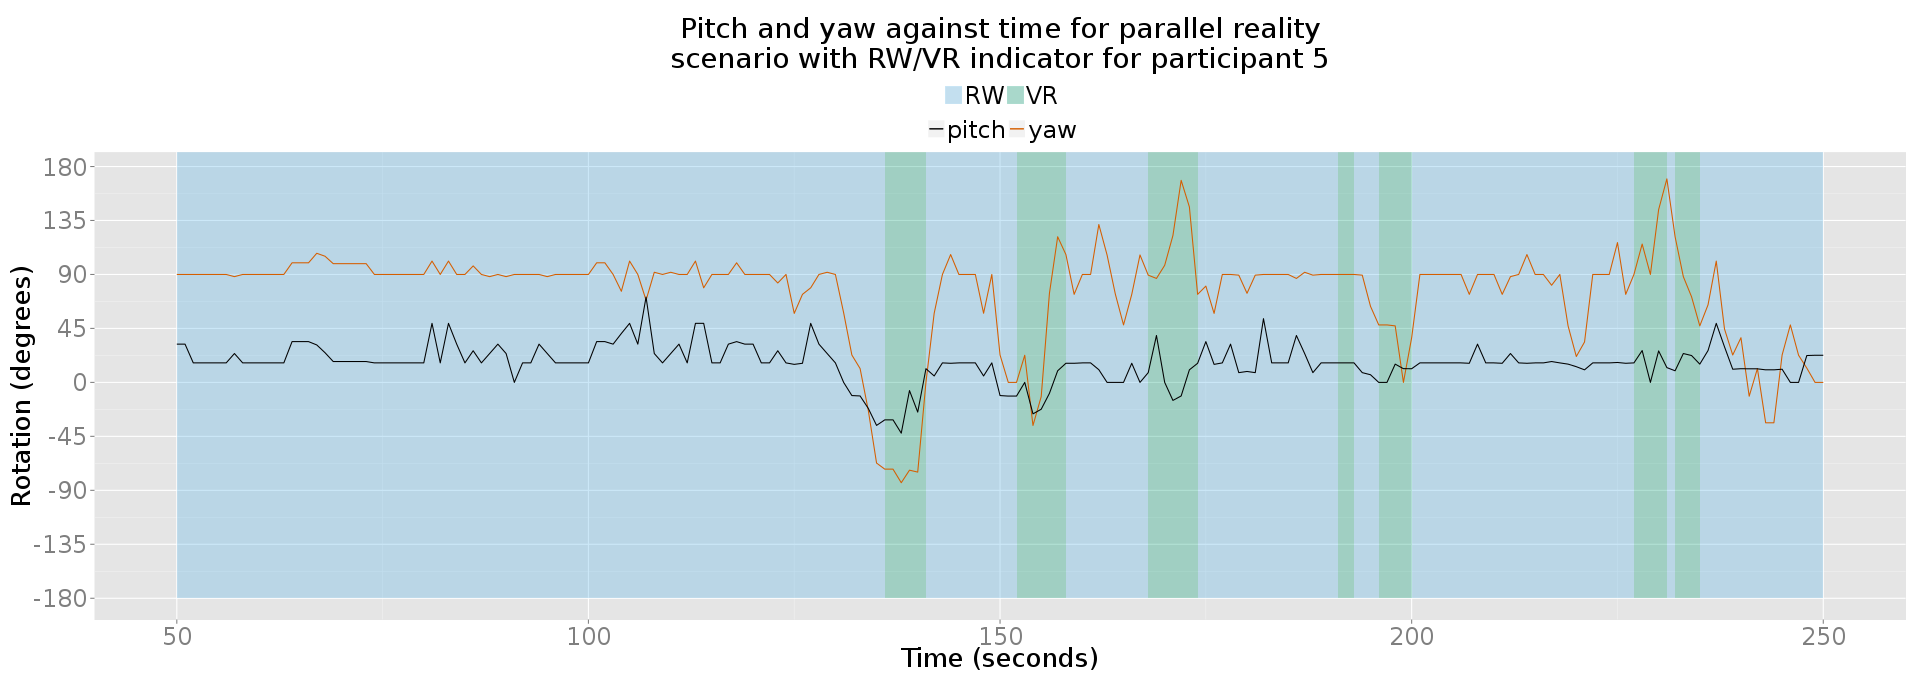
\includegraphics[width=\textwidth]{1/5_pitch_yaw.png}
	\caption{Pitch \& yaw against time for participant 5 in PR scenario.}
	\label{5_pitch_yaw.png}
	\end{center}
\end{figure}

Calculating the mean standard deviation in yaw, weighted by the duration of the periods, shows this relationship more concretely. With reference to the figures in table \ref{sdyawtab} the mean standard deviation in yaw while perceiving VR stimuli is substantially higher than while perceiving RW stimuli for participant 1 (39.887\textdegree compared to 25.545\textdegree) \& for participant 3 (60.636\textdegree compared to 11.702\textdegree). The values are however very close for participant 5, due to the initial large delta in yaw just before the first transition into VR at around 130 seconds. Recalculating the mean standard deviation from 150 seconds onwards to exclude this peak gives rise to the values of 36.074\textdegree for VR stimuli compared to 17.046\textdegree for RW stimuli.

Also, comparing yaw from the VR periods of the PR scenario (table \ref{sdpitchyawpr}) against yaw from the traditional scenario (table \ref{sdpitchyawtrad}) it can be seen that in most cases there is a noticeably less yaw change in the VR periods of the PR scenario than in the traditional scenario.

%=====================

Comparing between VR section of traditional scenario \& VR periods of PR scenario

Smaller difference between yaw \& pitch for VR periods of PR scenario than for VR segment of traditional scenario

Yaw change less in VR periods of PR scenario than in VR segment of traditional scenario

	Overall head movement in PR scenario VR periods lower than in VR segment of traditional scenario

%=====================


PR scenario against VR section of traditional scenario
PR scenario against VR \& RW section of traditional scenario

More yaw than pitch is true for all participants, even those that displayed a less pronounced difference in amount of movement between VR \& RW of PR scenario.

%=====================

Mean time spent in each environment for PR scenario varied greatly

%=====================

\textbf{***MOVEMENT} - you know, less head movement when position moving?



\textbf{Weighted mean standard deviation in pitch \& yaw for RW \& VR periods of PR scenario.}

\begin{table}
\begin{center}
\begin{minipage}[t]{.47\linewidth}
\begin{center}
\begin{tabular}{|c|c|c|}
\hline

\textbf{Participant} & \textbf{RW (\textdegree)} & \textbf{VR (\textdegree)} \\

\hline

1 & 13.325 & 17.554 \\

\hline

3 & 12.194 & 24.662 \\

\hline

4 & 6.133 & 6.133 \\

\hline

5 & 12.193 & 12.797 \\

\hline

6 & 15.712 & 15.349 \\

\hline
\end{tabular}
\caption{Weighted mean sd in pitch for PR scenario.}
\label{sdpitchtab}
\end{center}
\end{minipage}
%
\begin{minipage}[t]{.47\linewidth}
\begin{center}
\begin{tabular}{|c|c|c|}
\hline

\textbf{Participant} & \textbf{RW (\textdegree)} & \textbf{VR (\textdegree)} \\

\hline

1 & 25.545 & 39.887 \\

\hline

3 & 11.702 & 60.636 \\

\hline

4 & 18.032 & 15.300 \\

\hline

5 & 23.155 & 29.274 \\

\hline

6 & 41.717 & 47.440 \\

\hline
\end{tabular}
\caption{Weighted mean sd in yaw for PR scenario.}
\label{sdyawtab}
\end{center}
\end{minipage}
\end{center}
\end{table}










%=========================================================================================================

%\makebox[\textwidth][c]{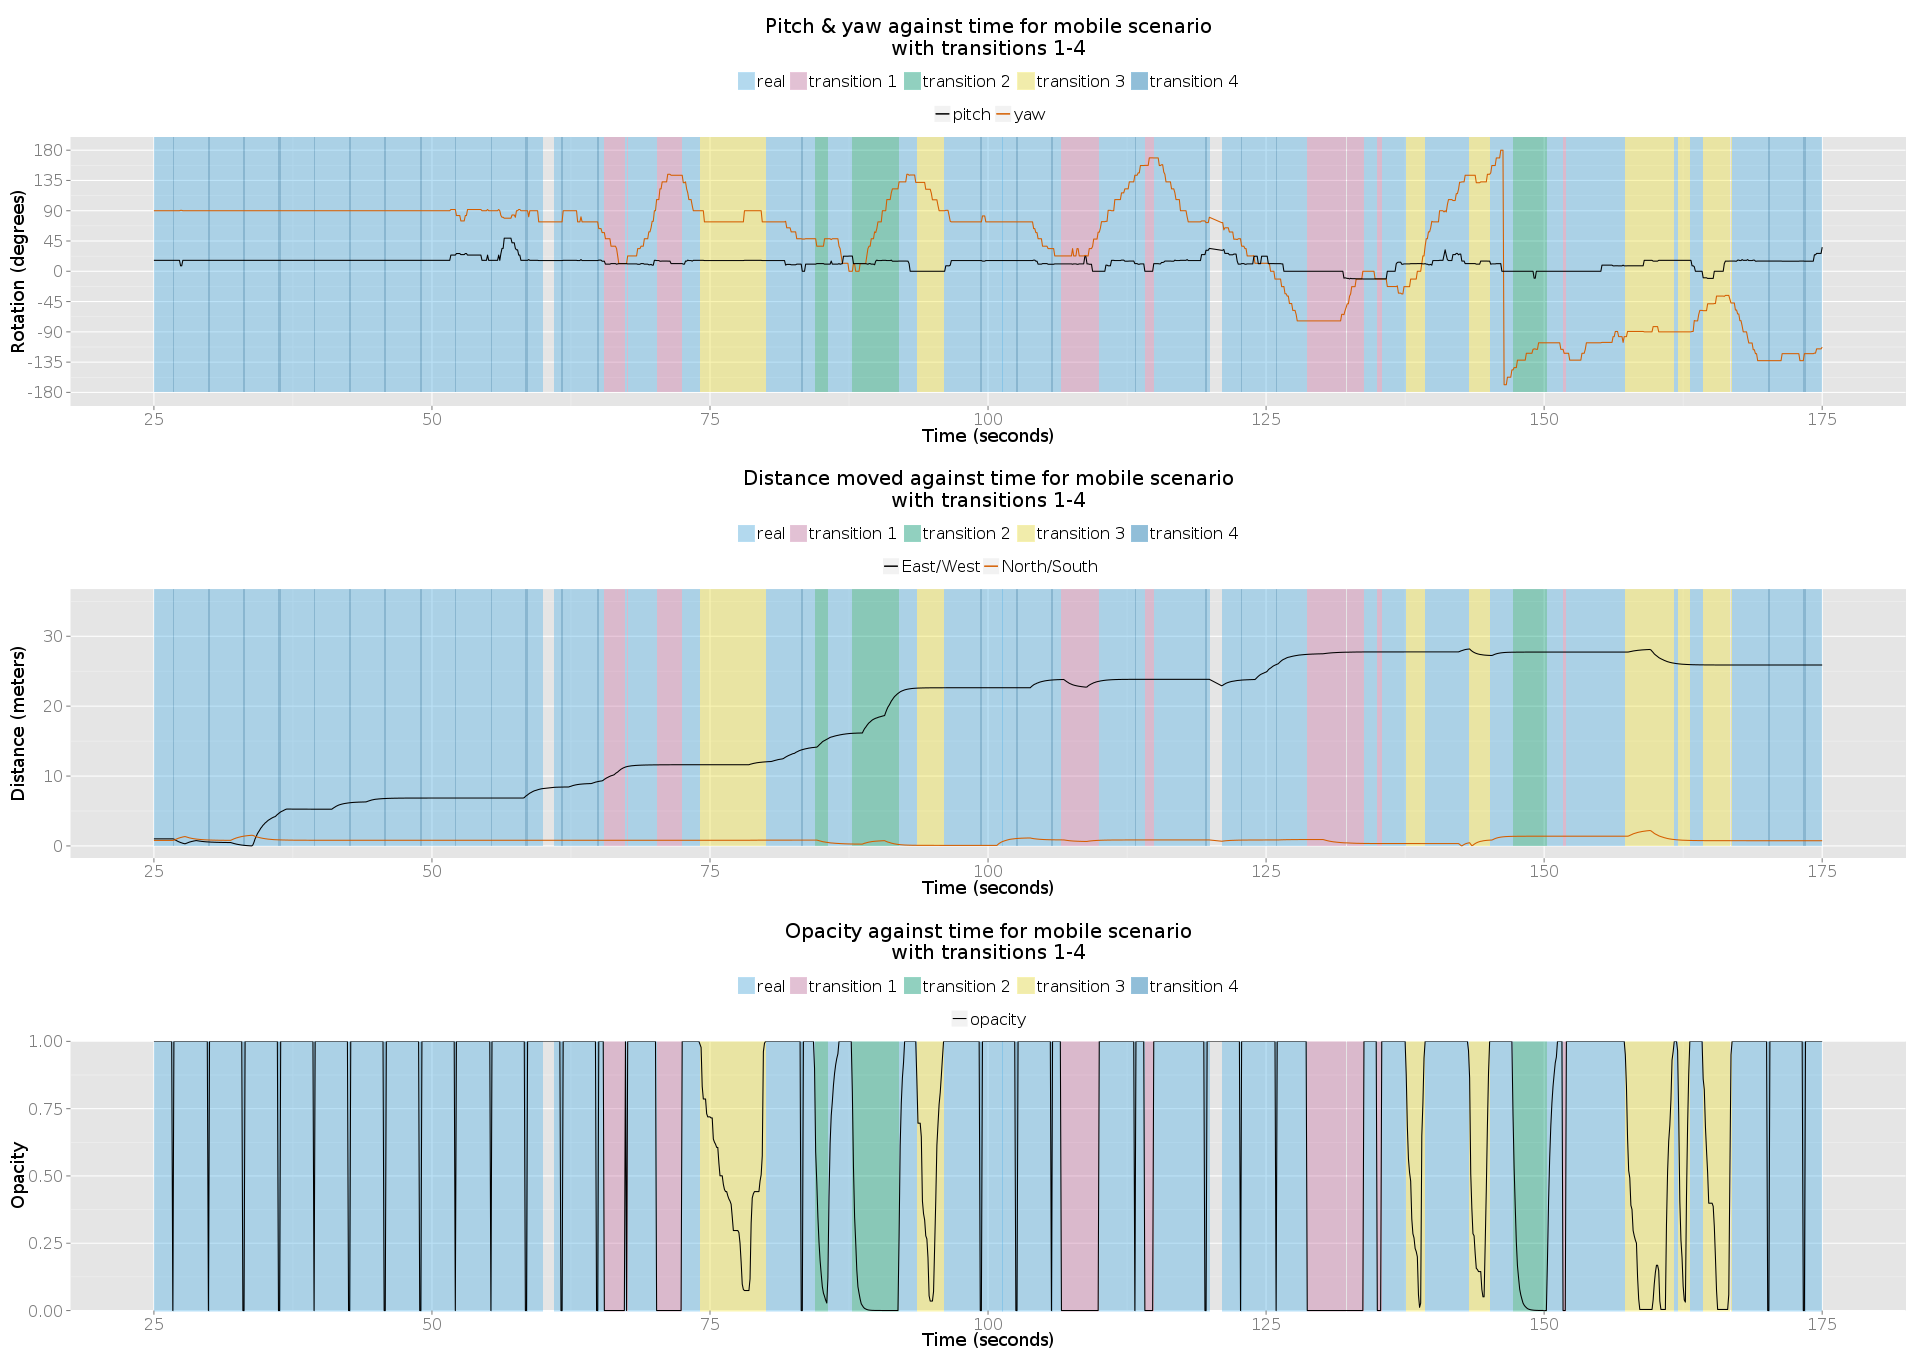
\includegraphics[width=1.2\textwidth]{2.1/11_1-4_3up.png}}

\clearpage

\subsection{Participant 1}

\begin{figure}[h]
	\begin{center}
	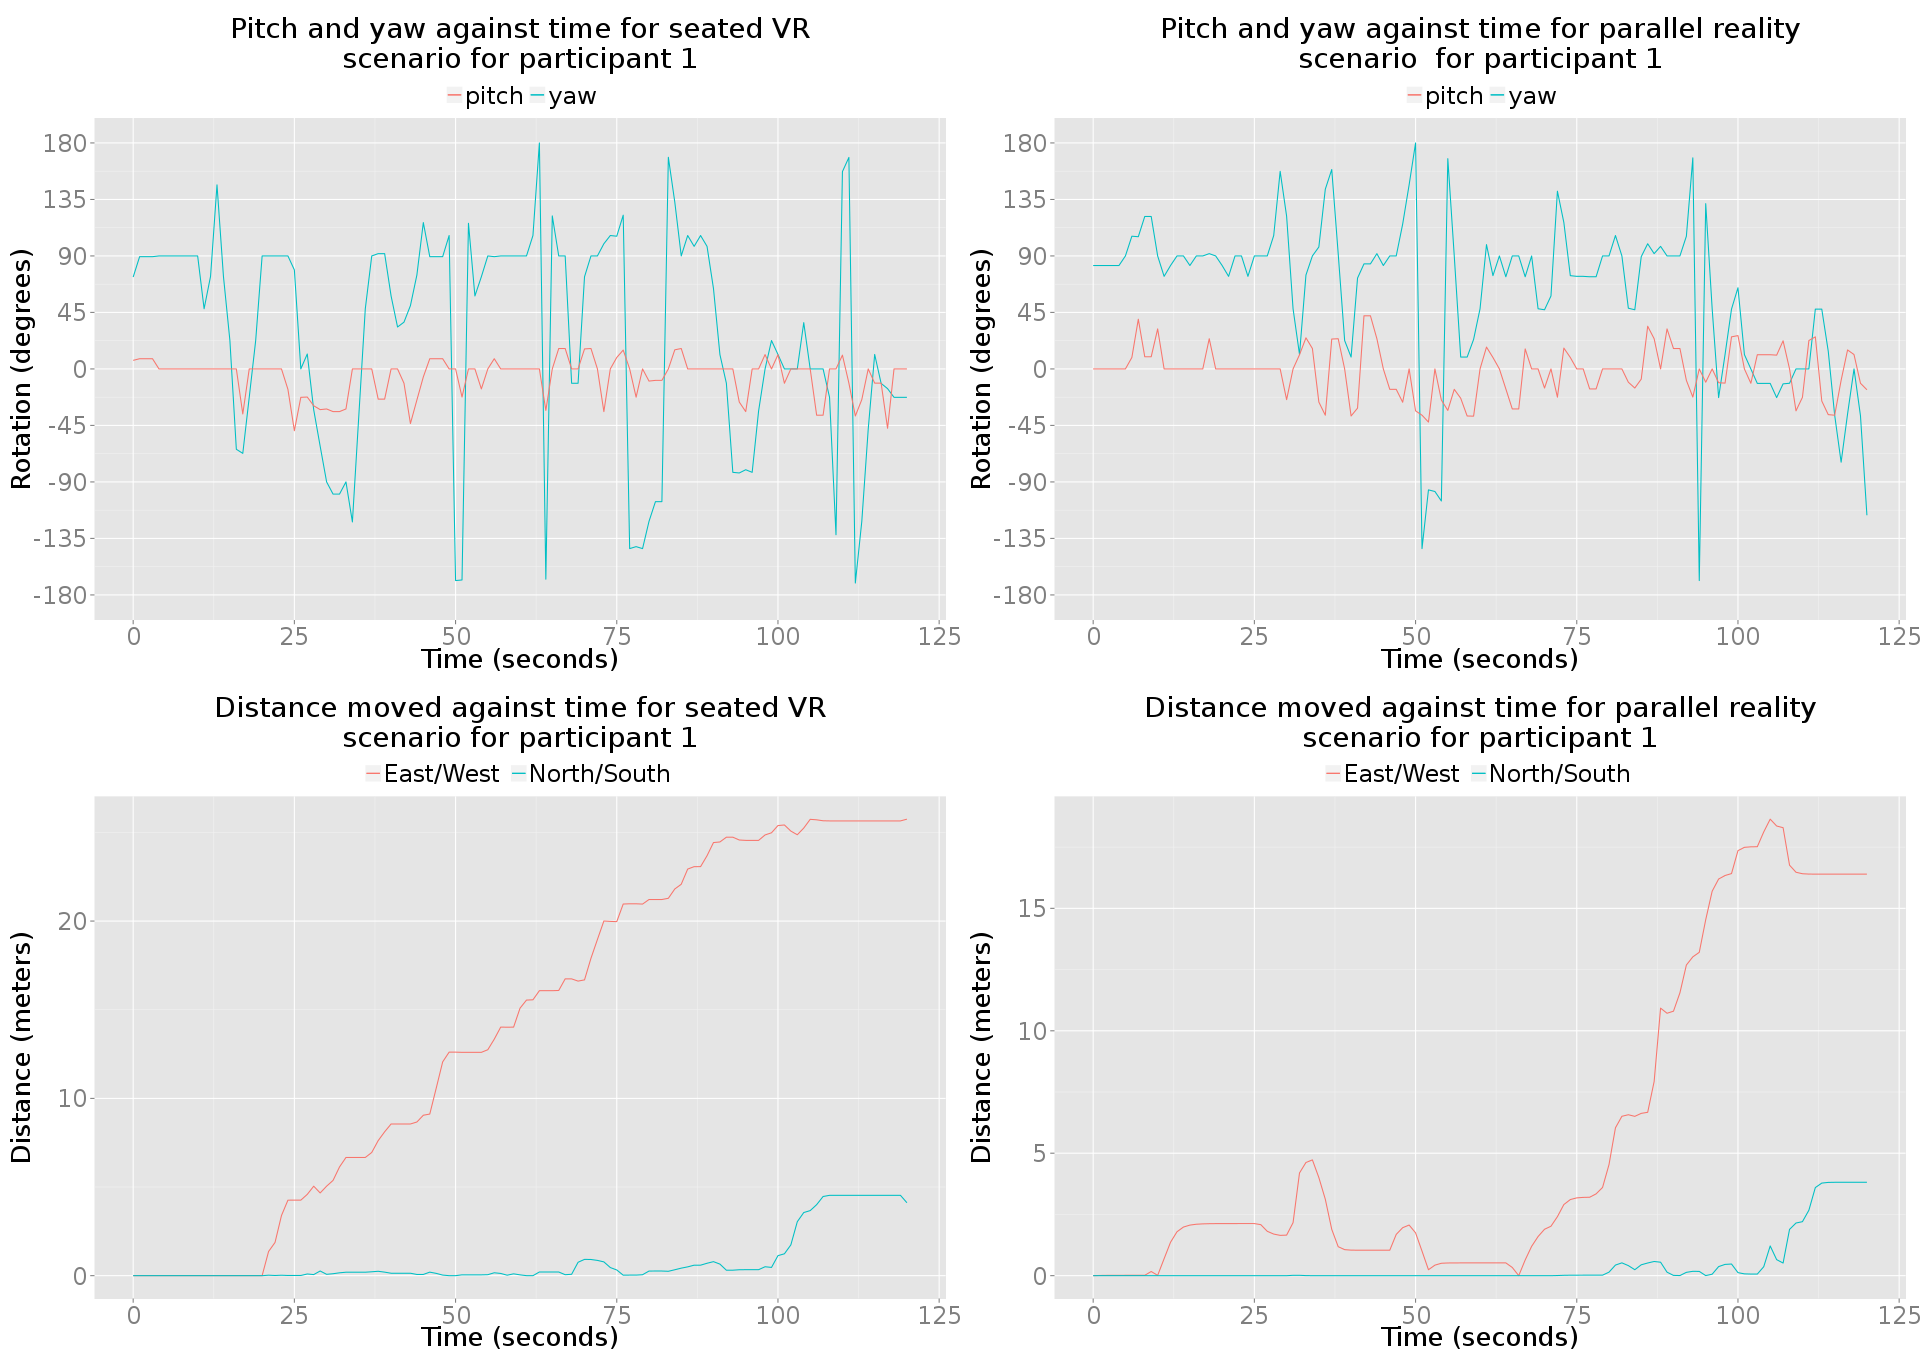
\includegraphics[width=\textwidth]{1/1_4up.png}
	\caption{Some images, yah.}
	\end{center}
\end{figure}

\clearpage

\begin{figure}[h]
	\begin{center}
	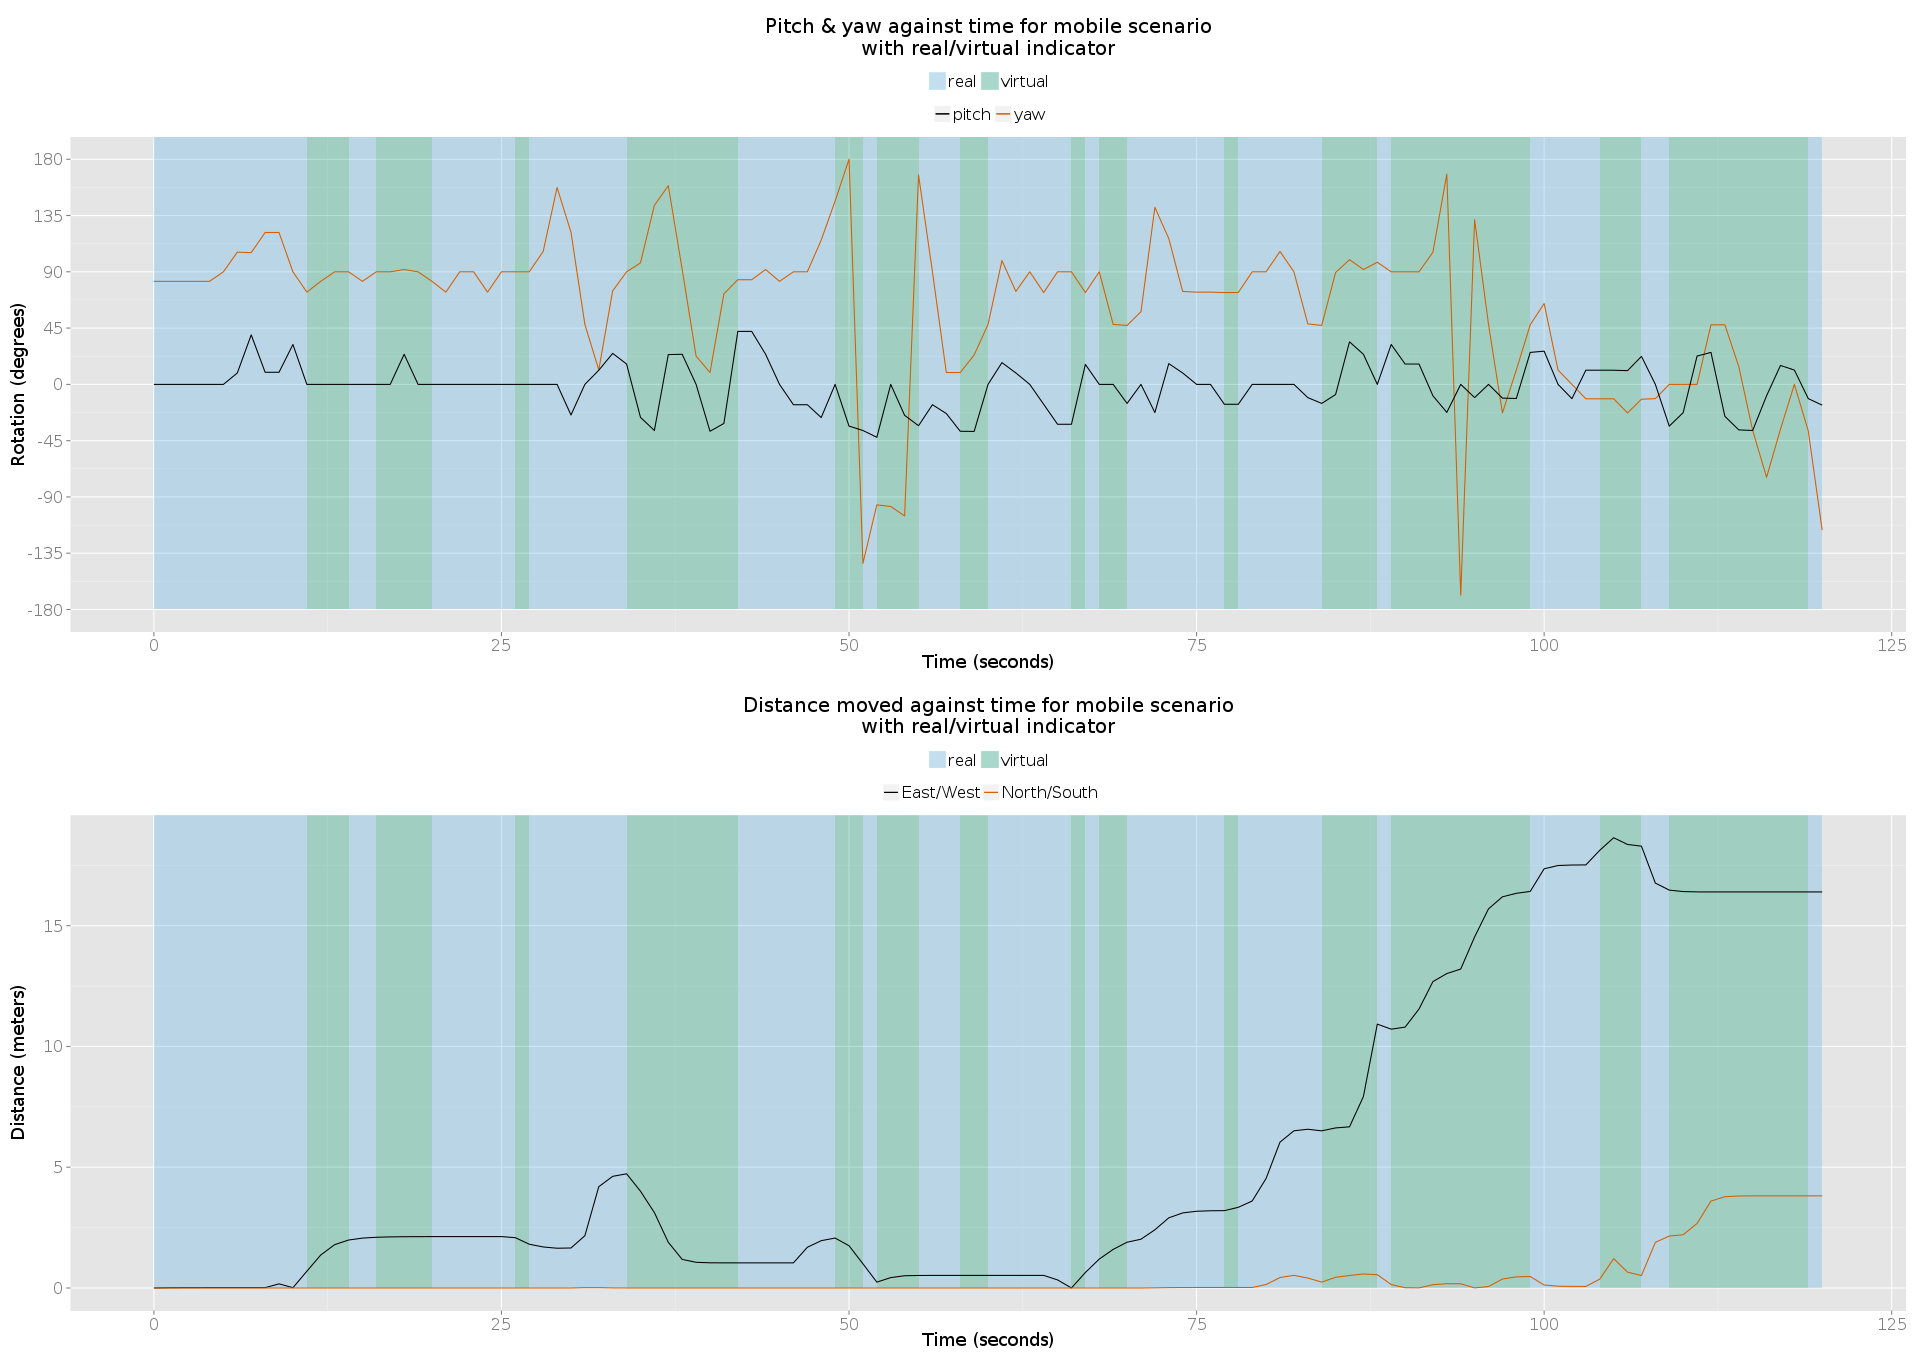
\includegraphics[width=\textwidth]{1/1_2up.png}
	\caption{Some images, yah.}
	\end{center}
\end{figure}

%=========================================================================================================

\clearpage

\subsection{Participant 3}

\begin{figure}[h]
	\begin{center}
	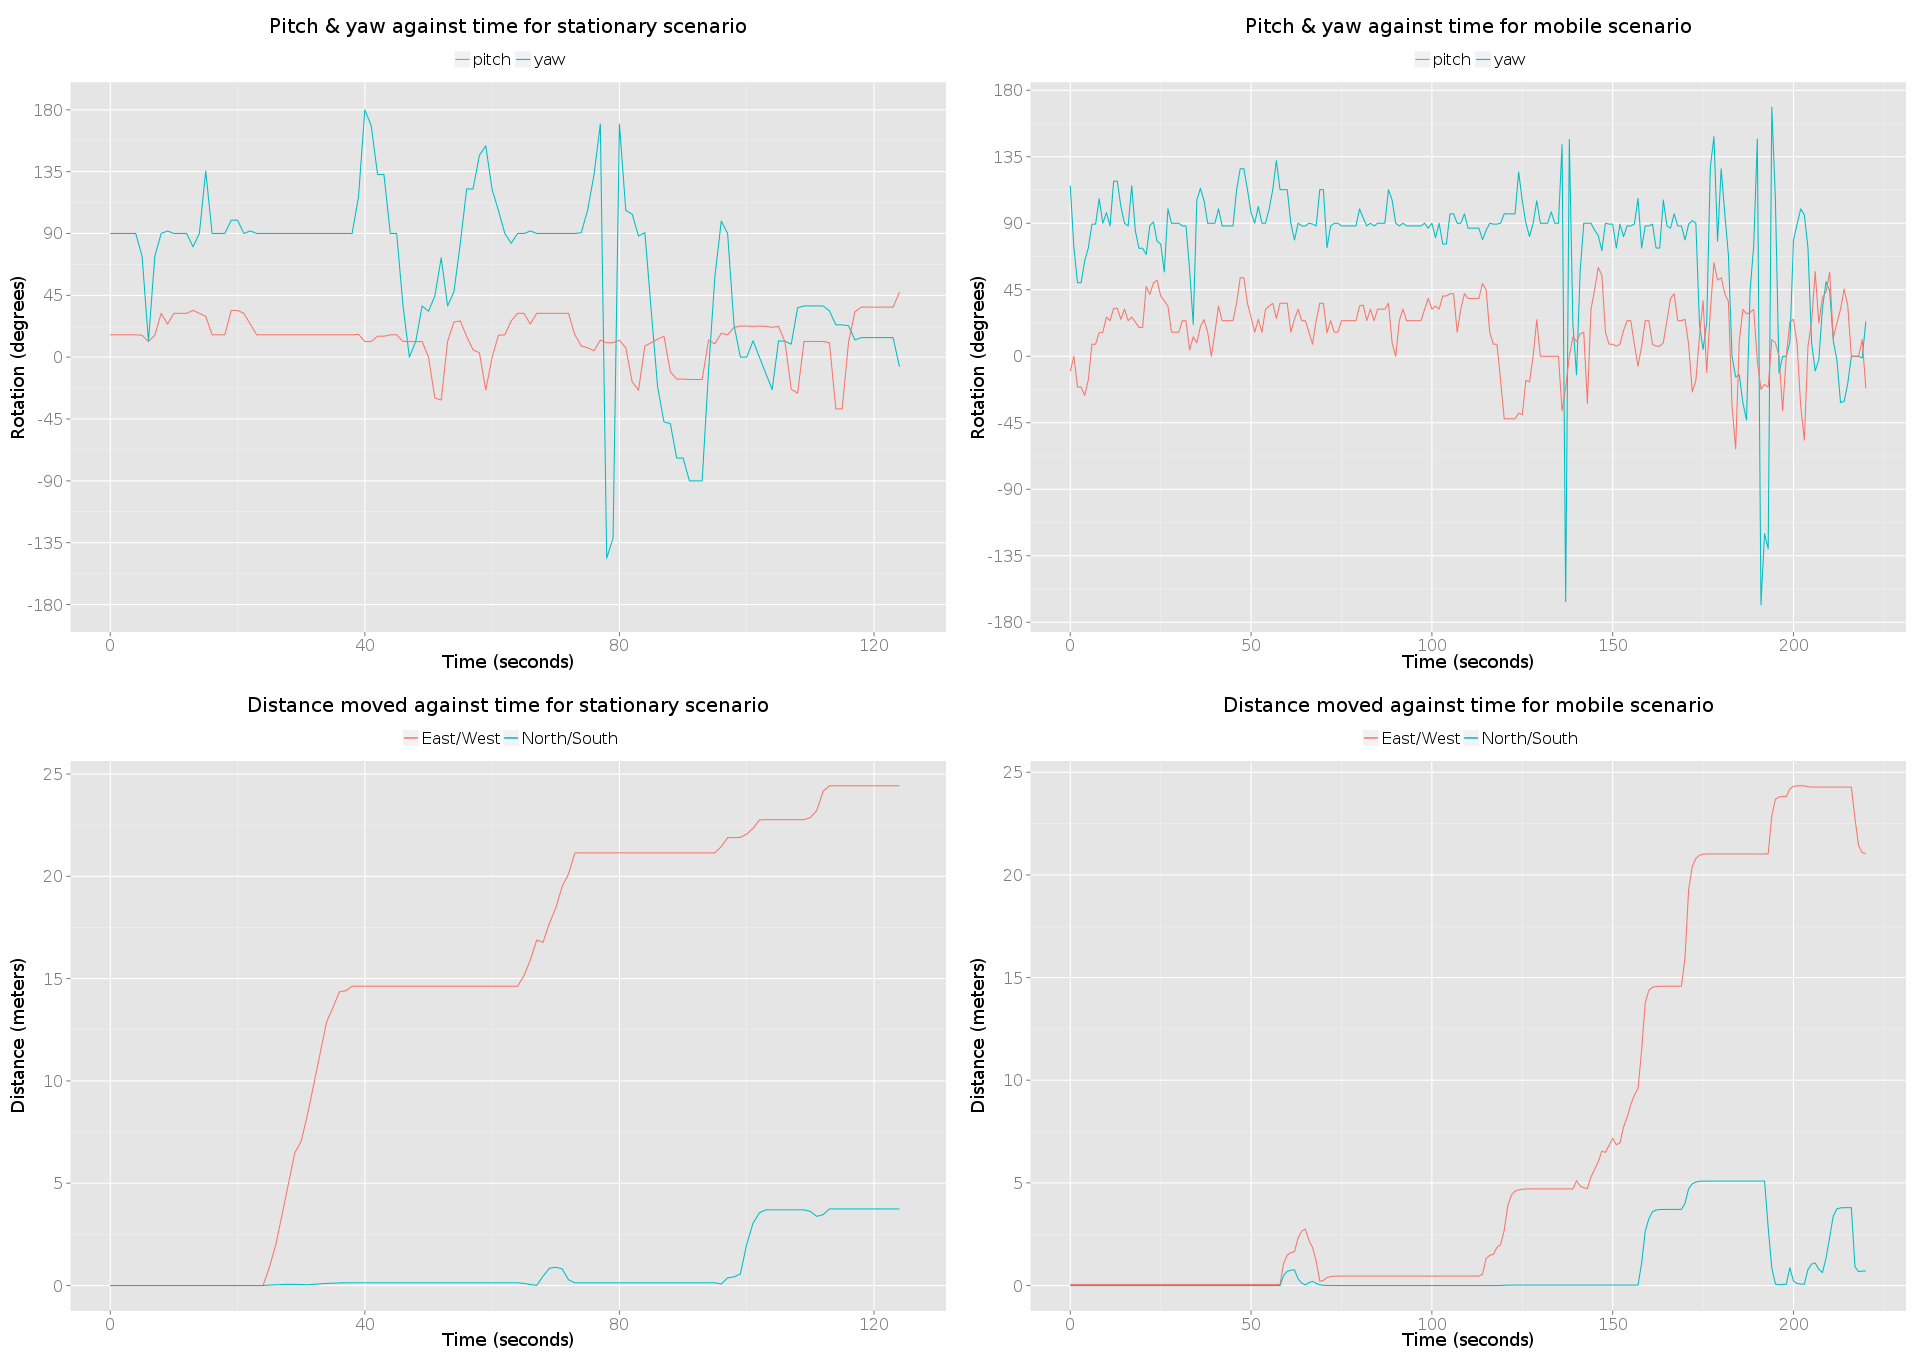
\includegraphics[width=\textwidth]{1/3_4up.png}
	\caption{Some images, yah.}
	\end{center}
\end{figure}

\clearpage

\begin{figure}[h]
	\begin{center}
	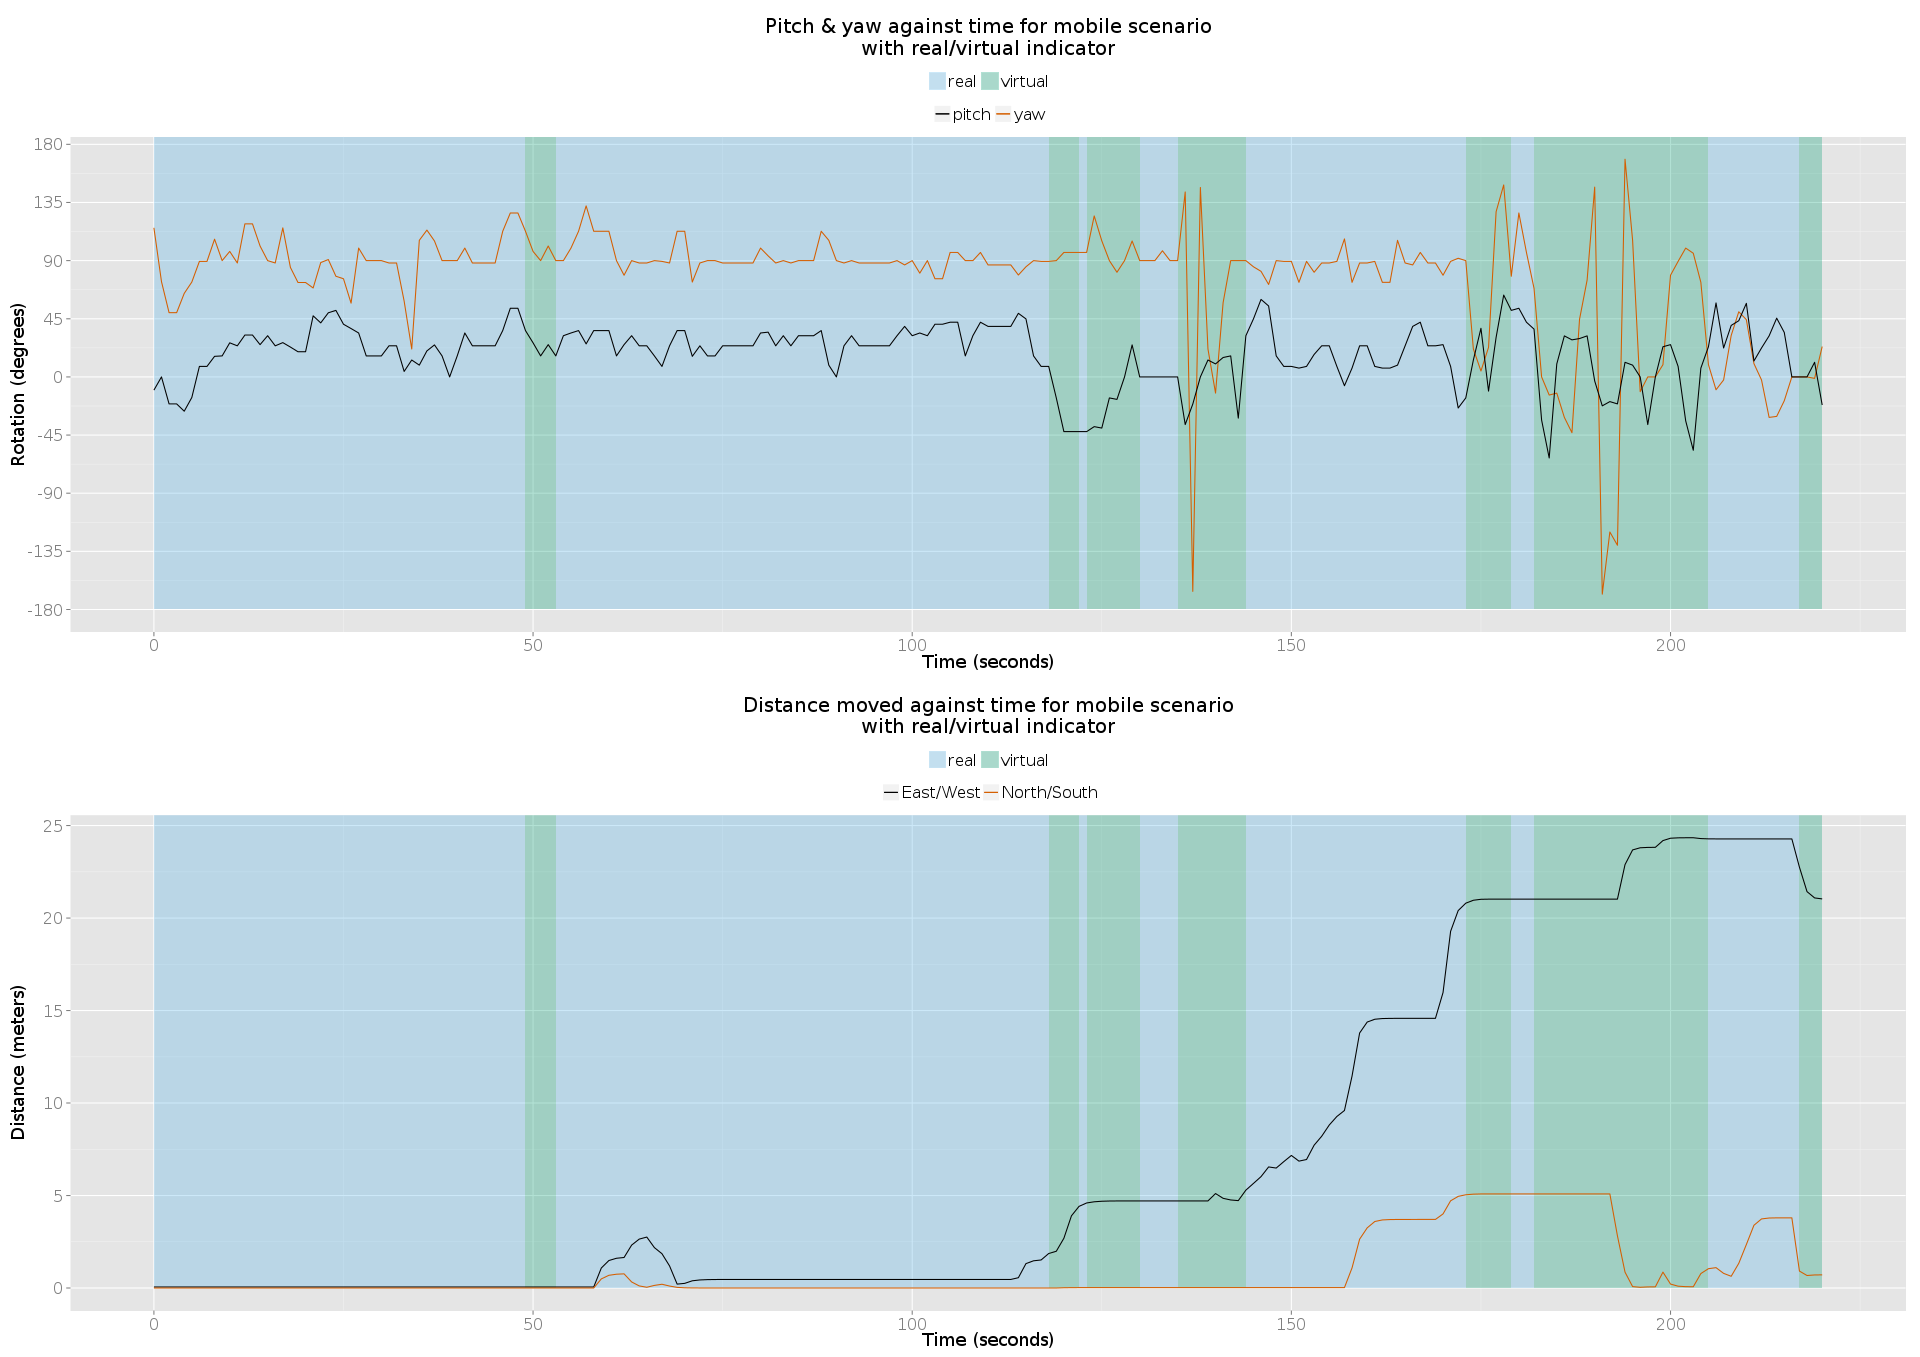
\includegraphics[width=\textwidth]{1/3_2up.png}
	\caption{Some images, yah.}
	\end{center}
\end{figure}

%=========================================================================================================

\clearpage

\subsection{Participant 4}

\begin{figure}[h]
	\begin{center}
	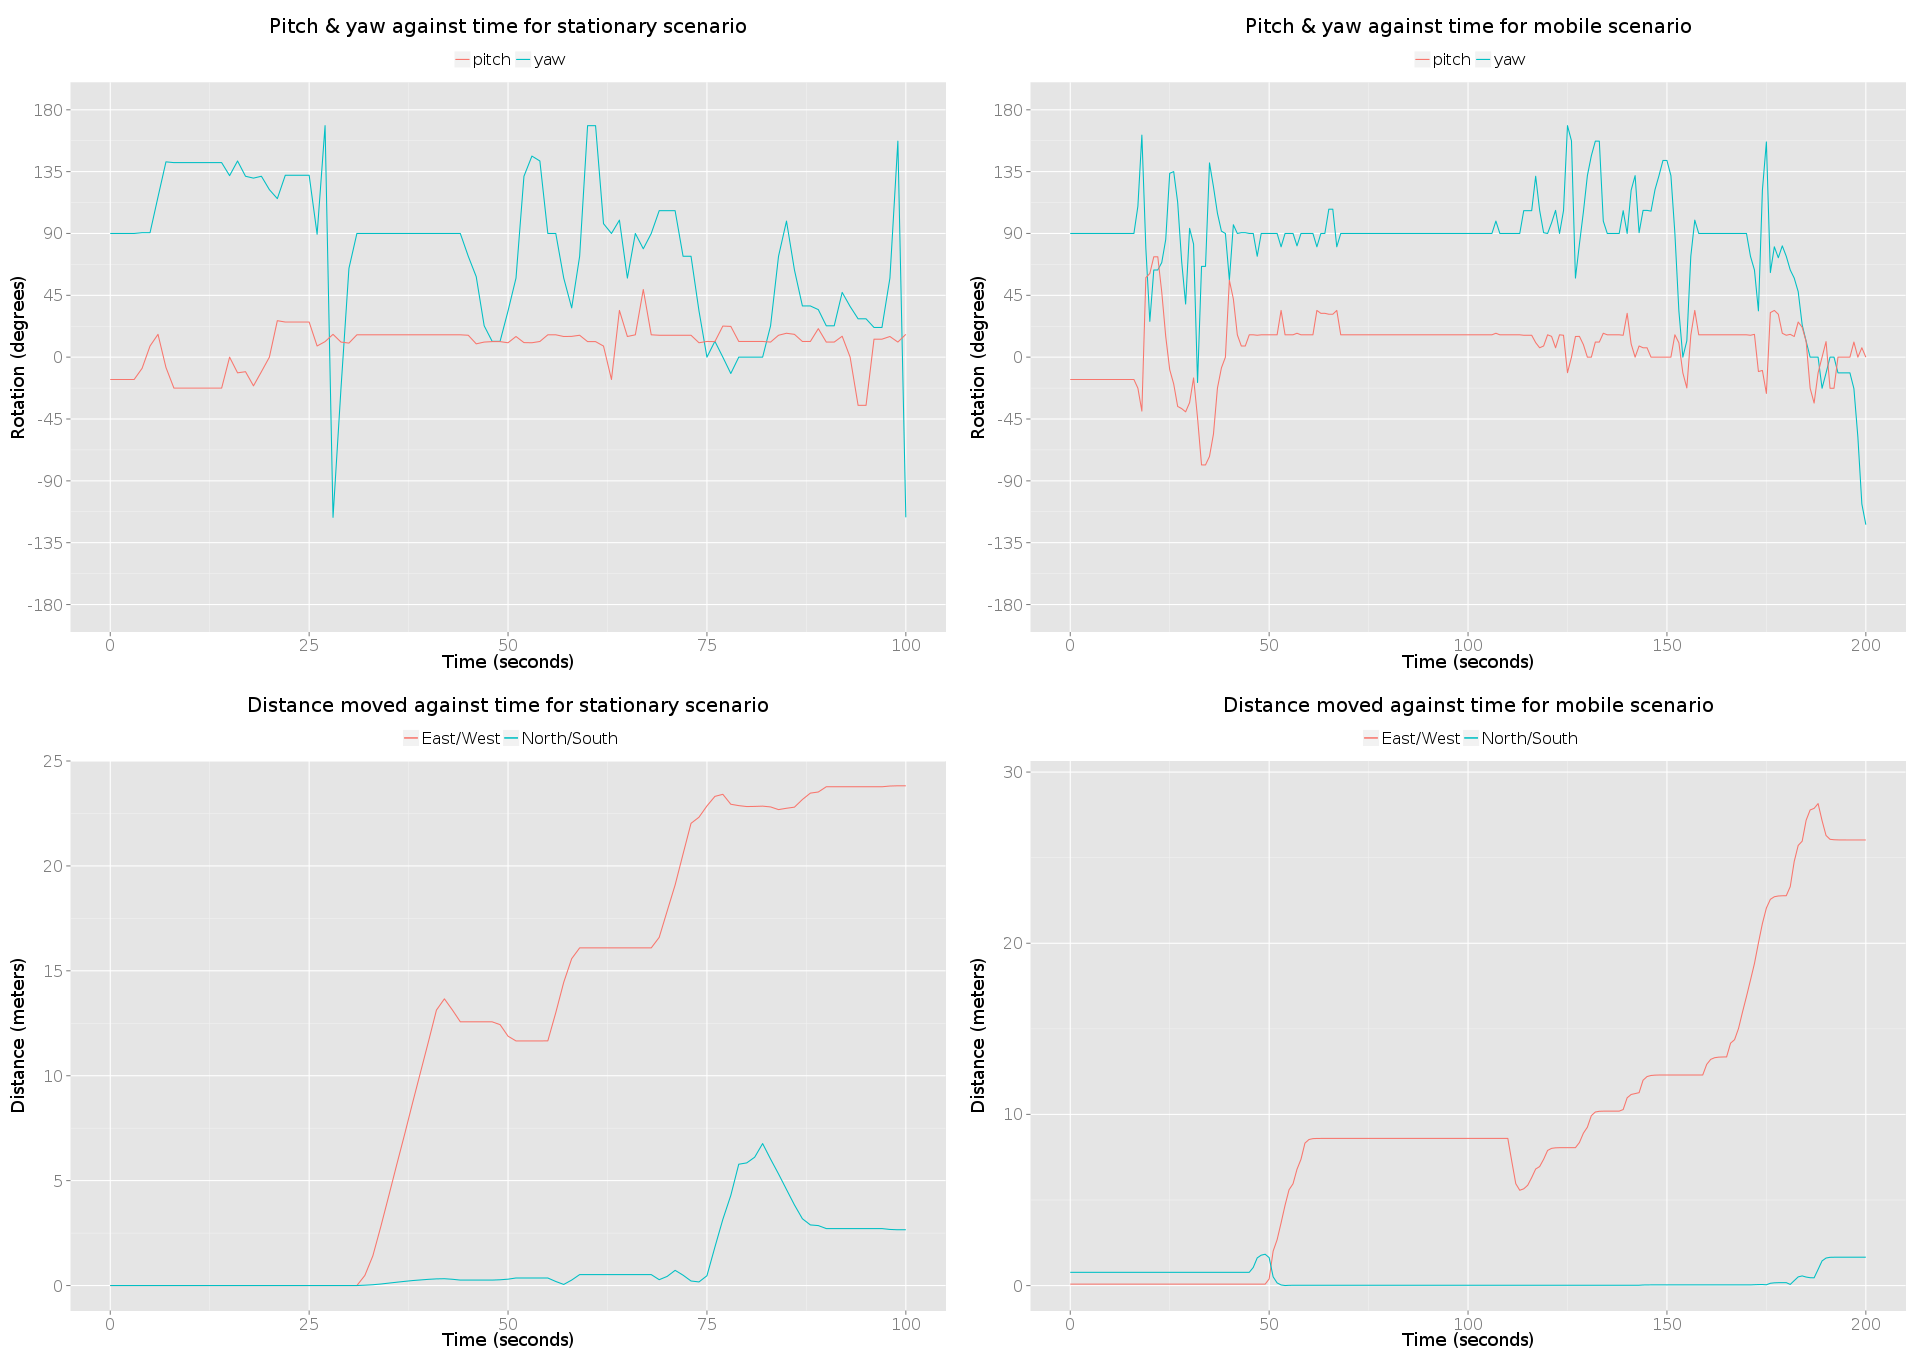
\includegraphics[width=\textwidth]{1/4_4up.png}
	\caption{Some images, yah.}
	\end{center}
\end{figure}

\clearpage

\begin{figure}[h]
	\begin{center}
	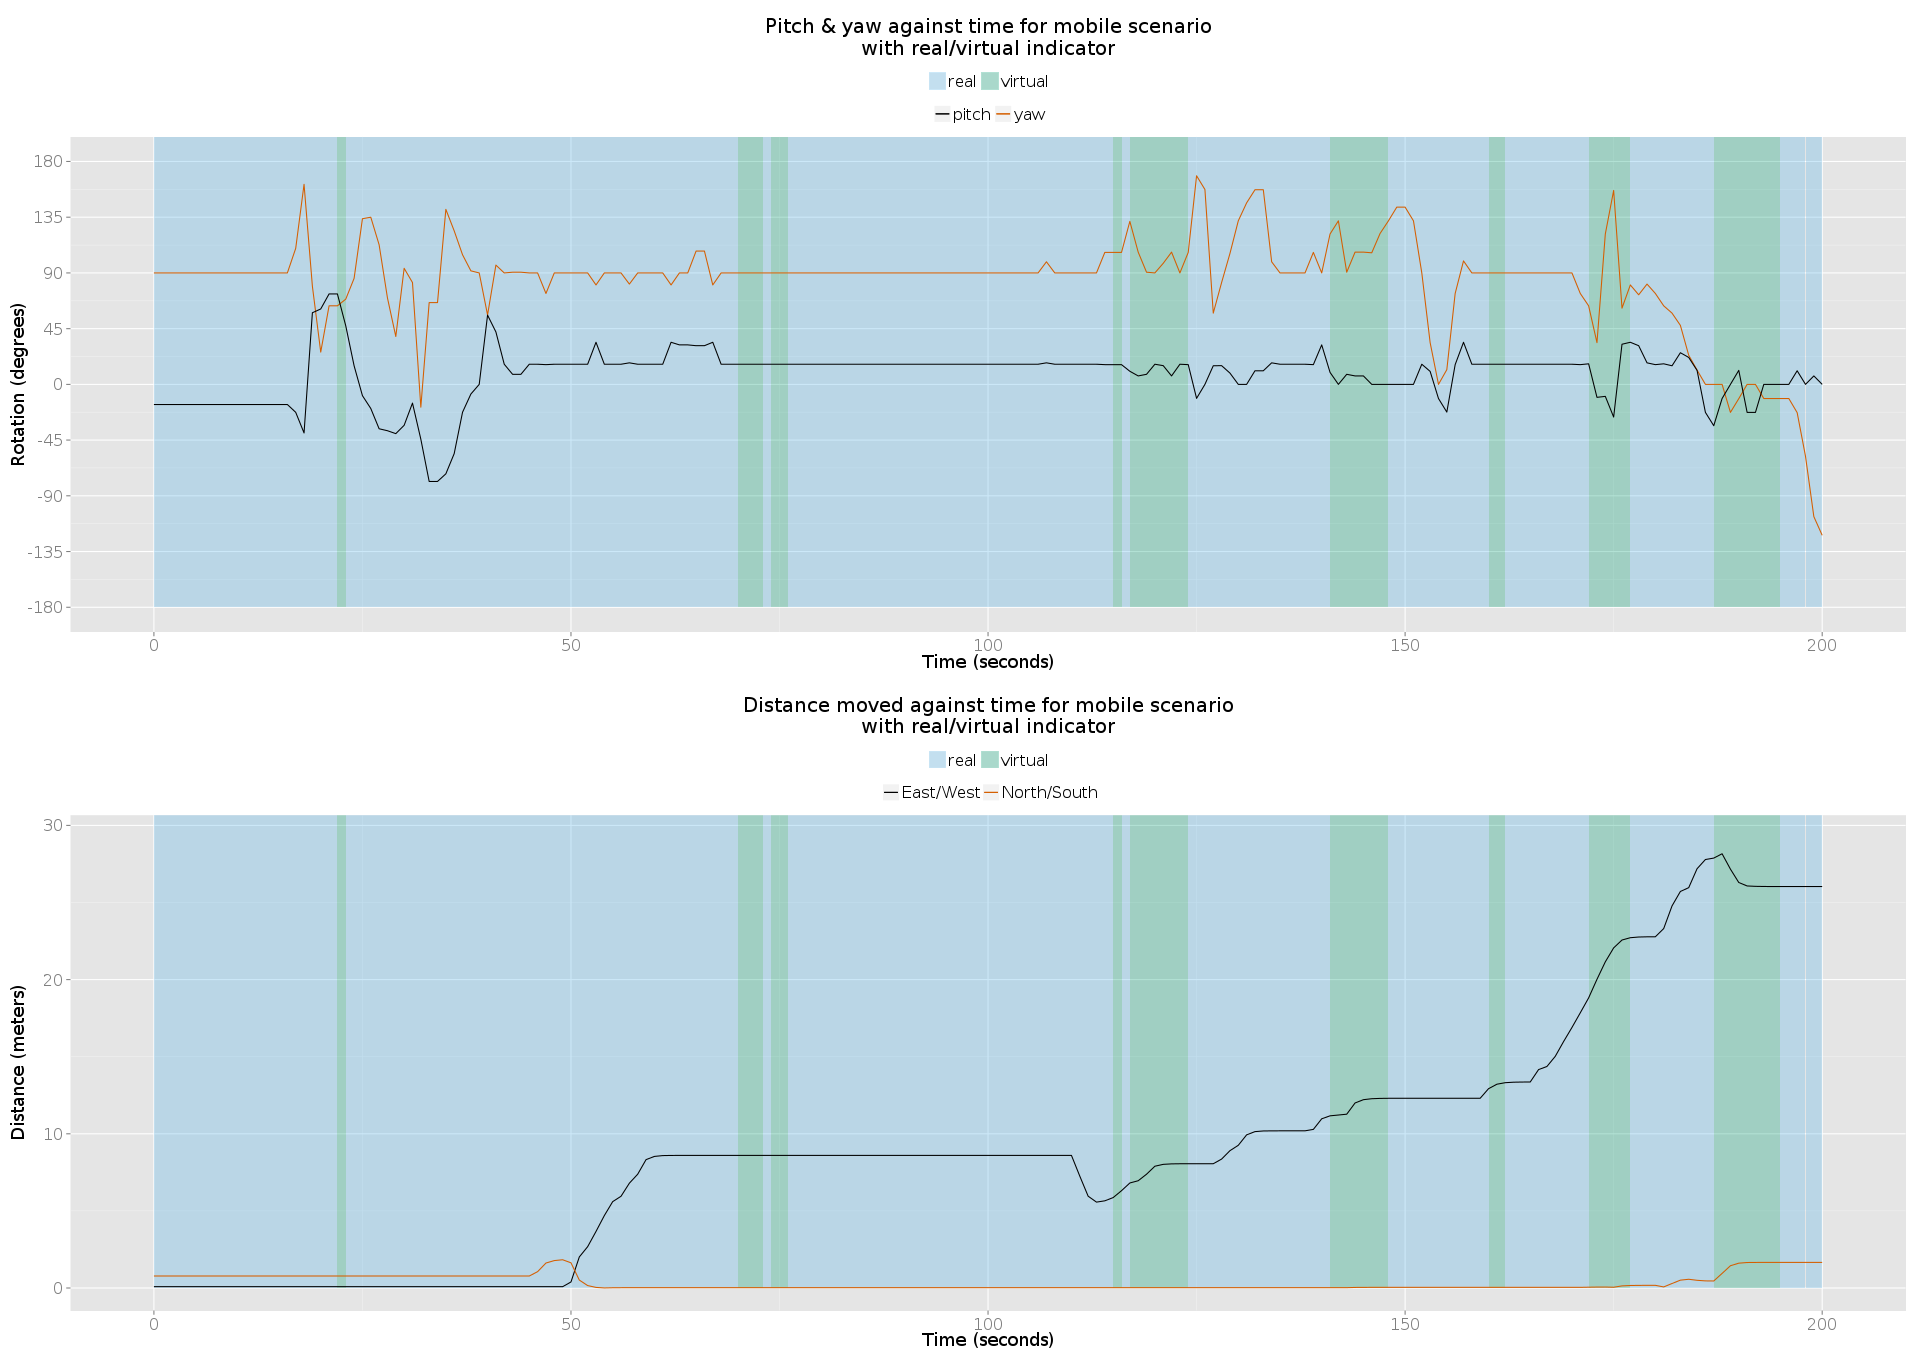
\includegraphics[width=\textwidth]{1/4_2up.png}
	\caption{Some images, yah.}
	\end{center}
\end{figure}

%=========================================================================================================

\subsection{Participant 5}

\clearpage

\begin{figure}[h]
	\begin{center}
	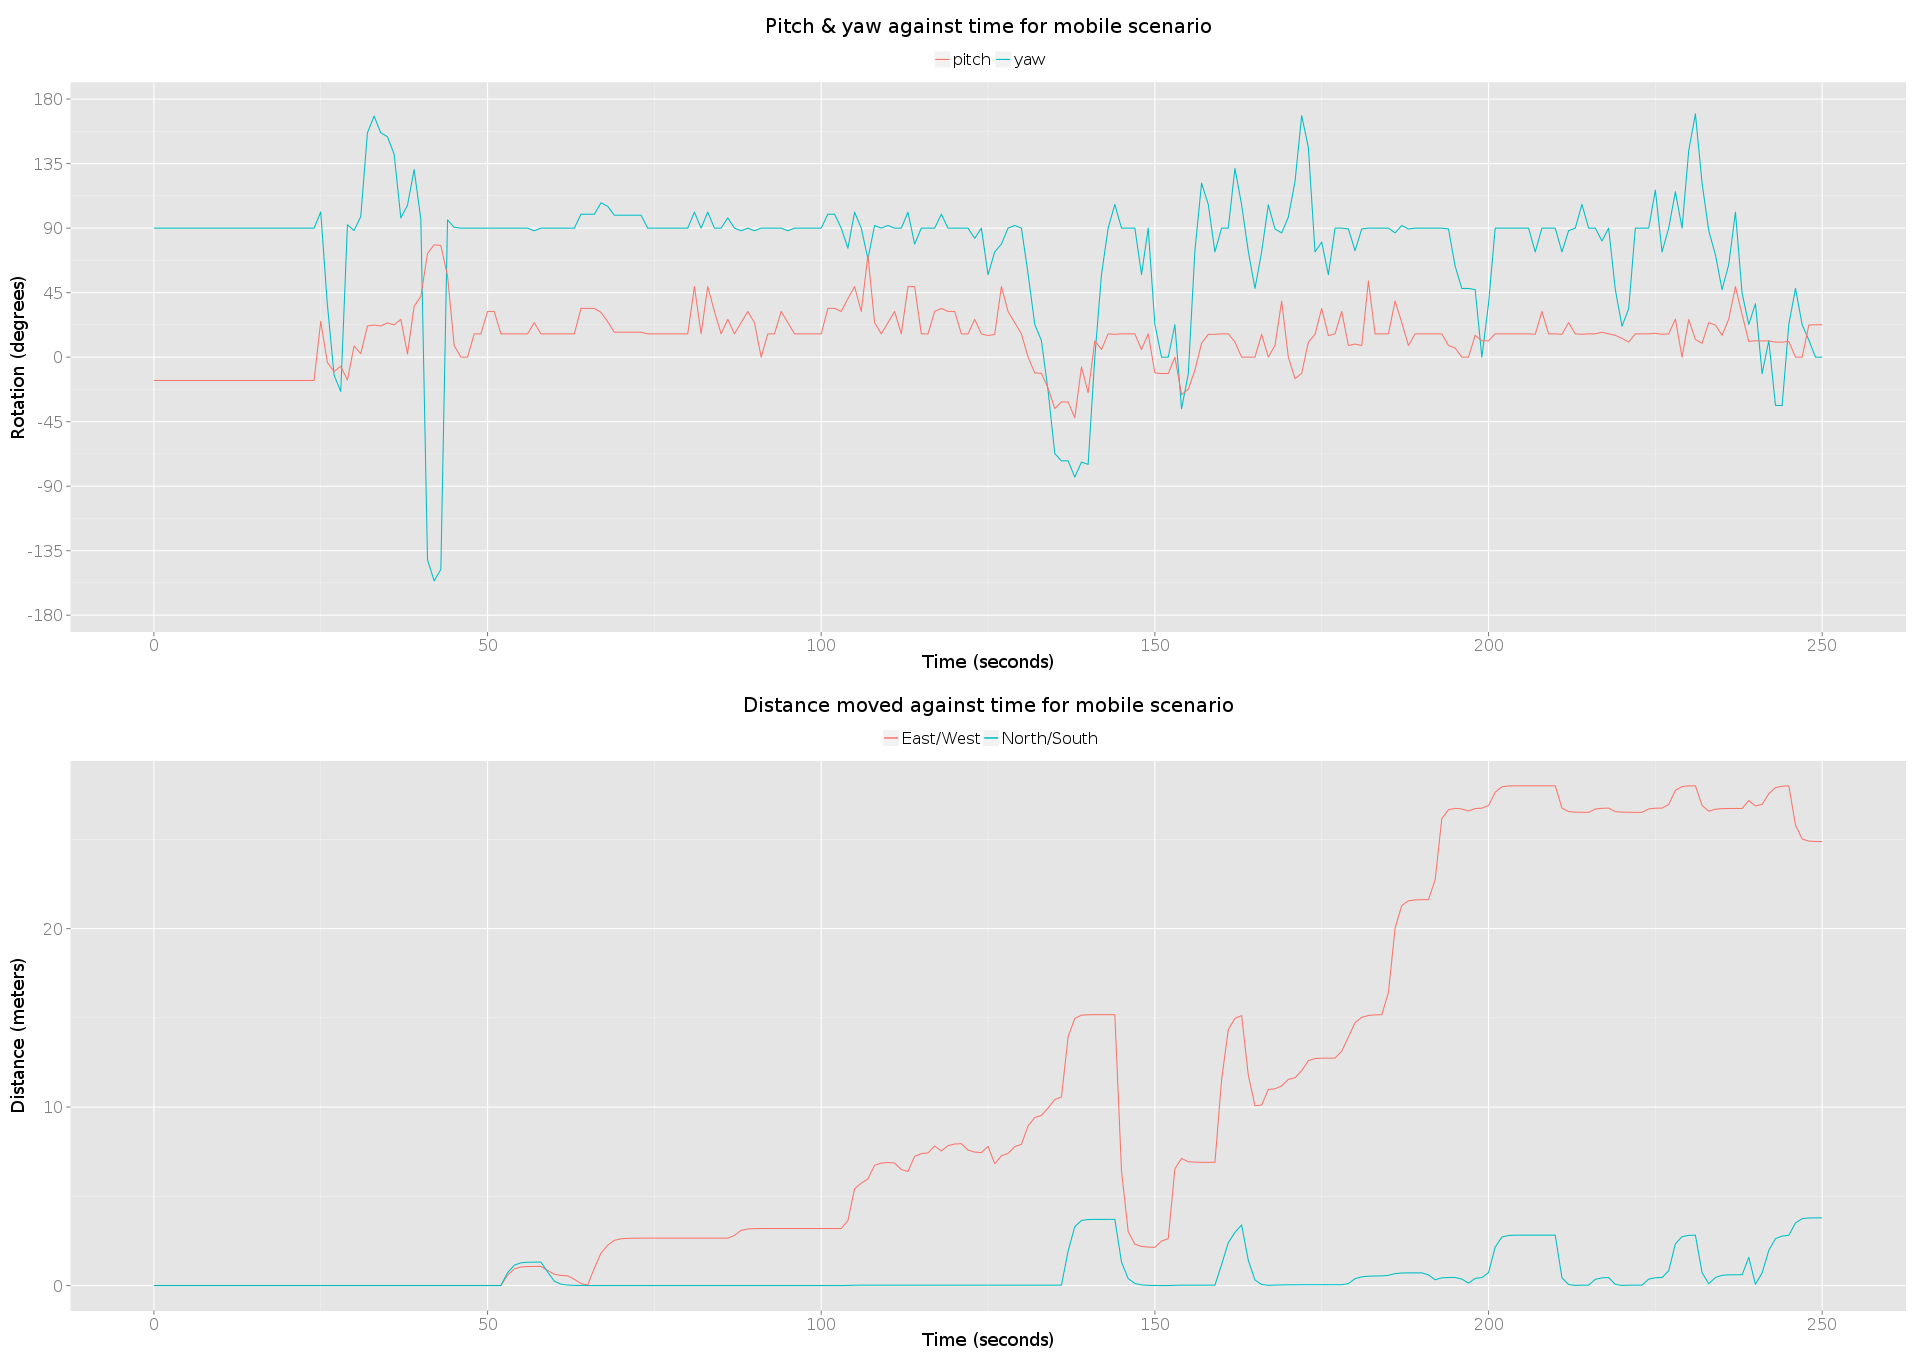
\includegraphics[width=\textwidth]{1/5_4up.png}
	\caption{Some images, yah.}
	\end{center}
\end{figure}

\clearpage

\begin{figure}[h]
	\begin{center}
	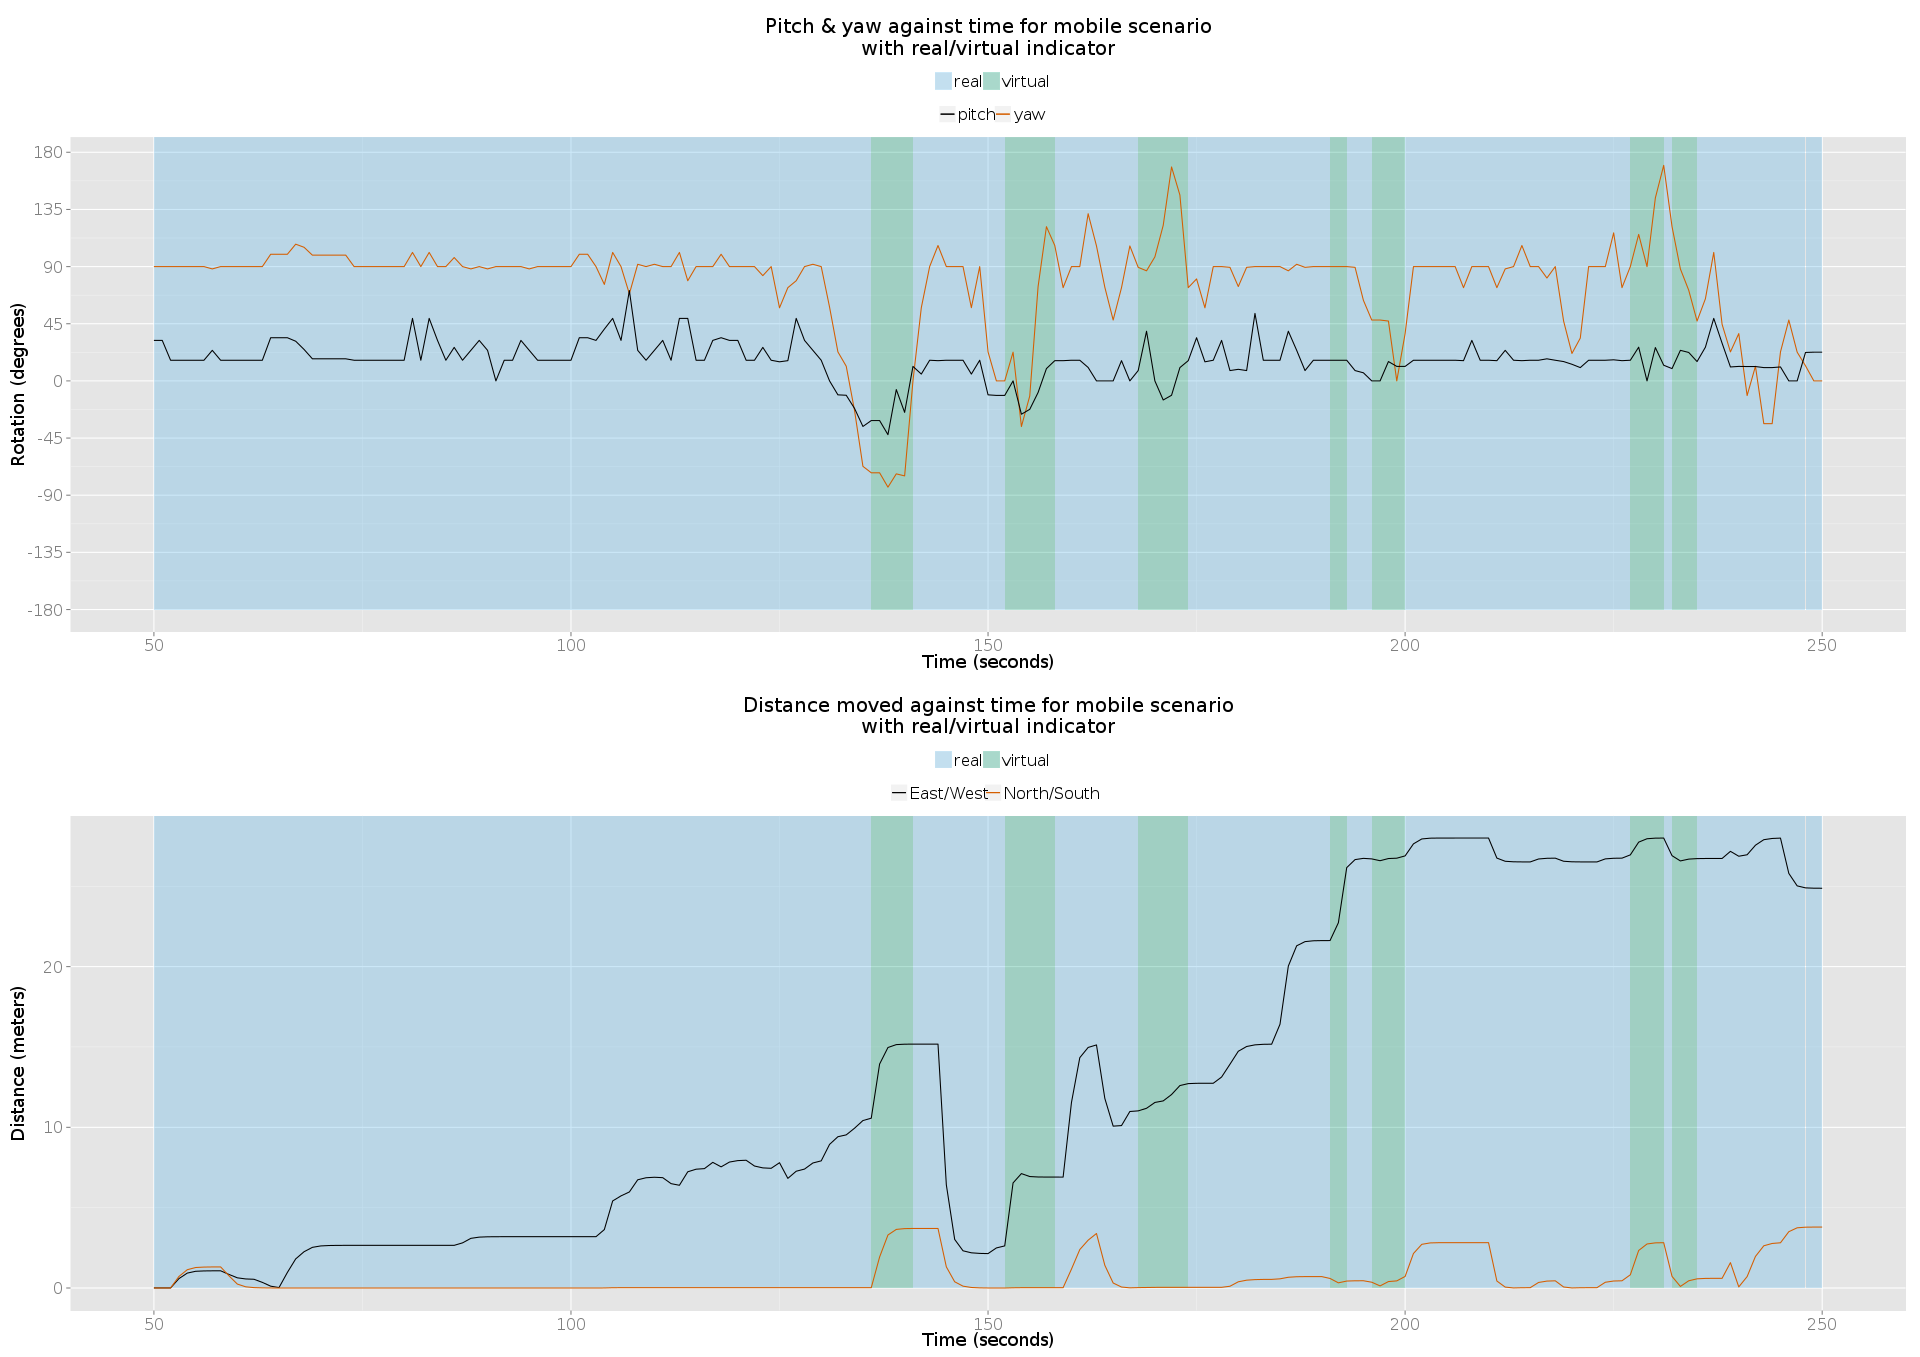
\includegraphics[width=\textwidth]{1/5_2up.png}
	\caption{Some images, yah.}
	\end{center}
\end{figure}

%=========================================================================================================

\subsection{Participant 6}

\clearpage

\begin{figure}[h]
	\begin{center}
	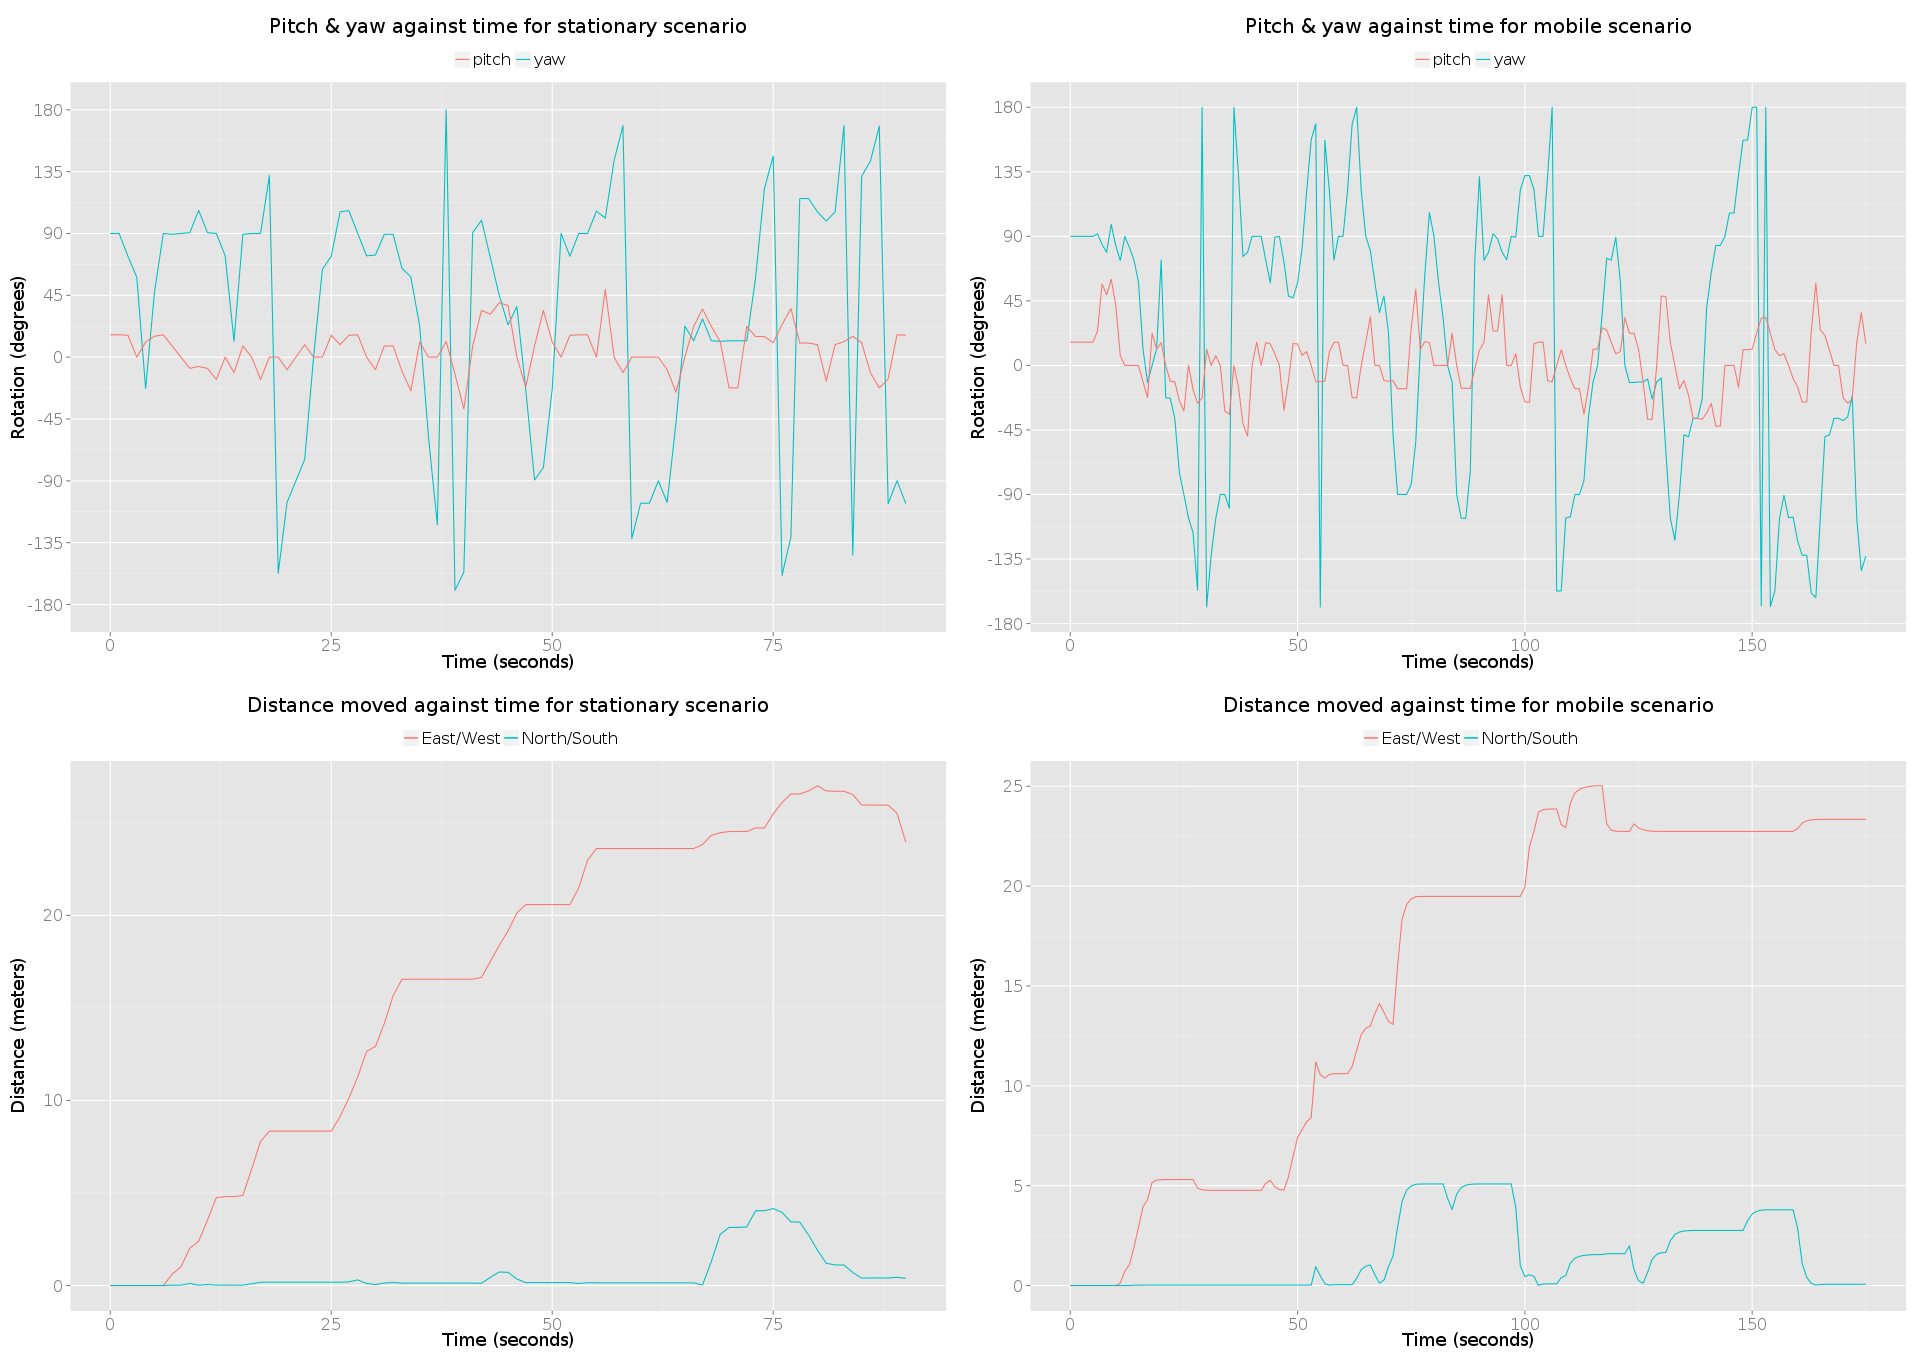
\includegraphics[width=\textwidth]{1/6_4up.png}
	\caption{Some images, yah.}
	\end{center}
\end{figure}

\clearpage

\begin{figure}[h]
	\begin{center}
	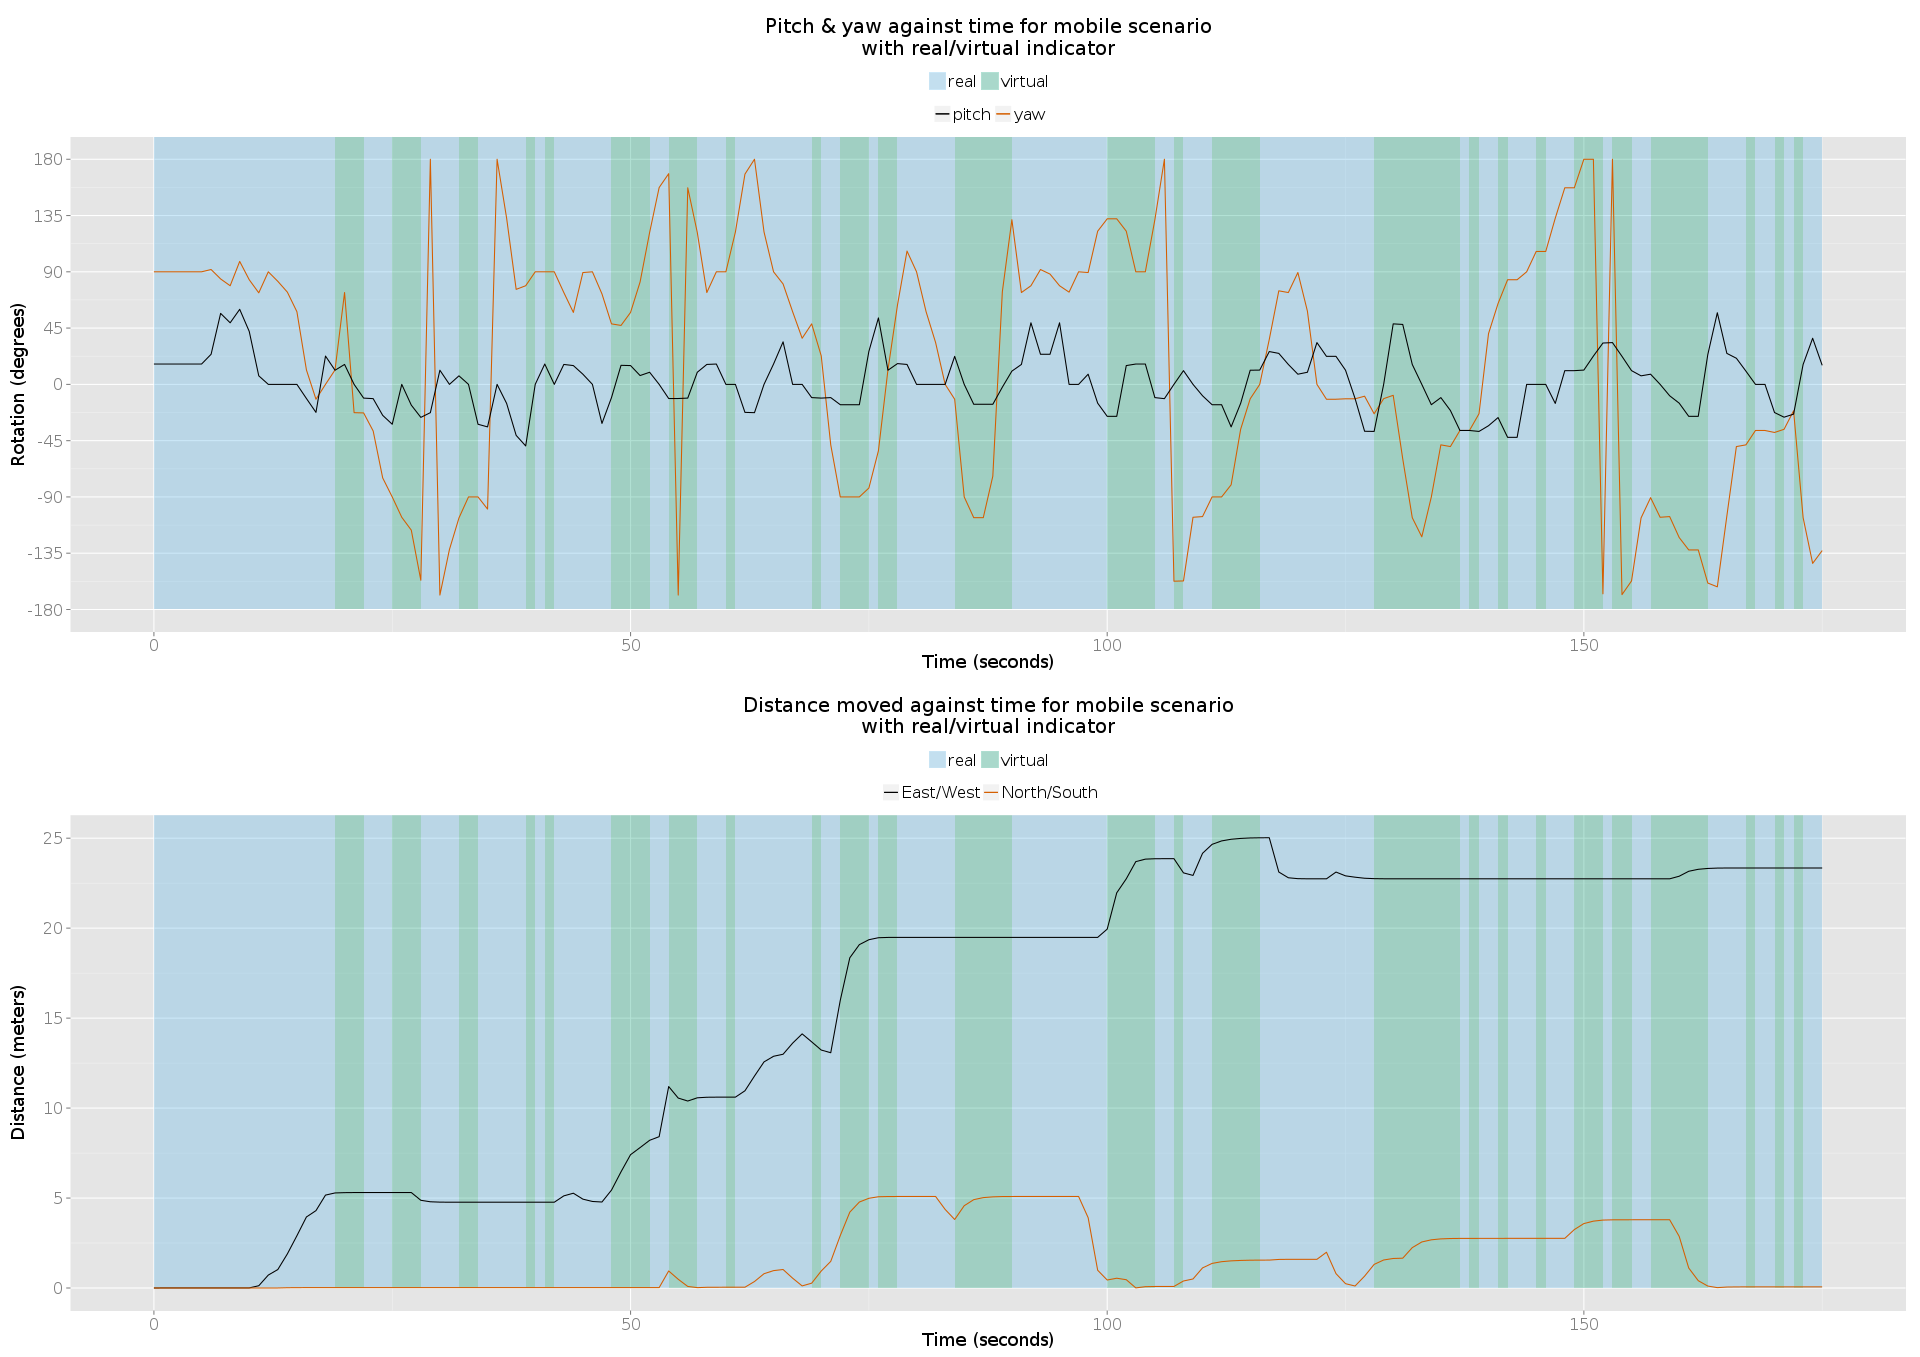
\includegraphics[width=\textwidth]{1/6_2up.png}
	\caption{Some images, yah.}
	\end{center}
\end{figure}

%=========================================================================================================





















%=========================================================================================================
%=========================================================================================================
%=========================================================================================================
%=========================================================================================================
%=========================================================================================================
%=========================================================================================================
%=========================================================================================================

\clearpage

\section{Stage 2}

\subsection{Evaluation}

Evaluating users' preferences toward different methods of transitioning between visual stimuli in different situations pertains to studying their reactions \& responses to ascertain the effect upon their focus of attention, concepts which are largely psychological in nature \& highly subjective~\cite{Ijsselsteijn2001}. Thus, subjective measures will produce the bulk of the data for evaluation. However, objective data will also be collected \& cross referenced with the subjective data in attempts to support or contradict any relationships that are identified.

It is hypothesized that a manner of transitioning between visual stimuli which results in a less severe BIP will be preferable to a manner of transitioning which results in a worse BIP. As focus in the Waterworth model is most closely related to presence in the VR literature~\cite{Waterworth2001}, one of the subjective measures that will be used in this evaluation will be an established presence measure, to try to capture the behaviour of the user's position upon the focus axis.

\subsubsection{Subjective Quantitative - Post-Task Questionnaire}
After completing the task, participants will respond to the Igroup Presence Questionnaire (IPQ)~\cite{Schubert2001} (see appendix \ref{ipqitems} for the items of the IPQ) which will provide subjective quantitative insight into their experiences with the system, in particular in relation to their position upon the focus axis of the combined model. The IPQ represents a useful questionnaire for evaluation of users' subjective experiences of using the Mirrorshades platform because its terms, especially in the `spatial involvement' scale, question about the RW environment in a manner that does not explicitly present it as a `distraction' from the VR interaction as many other presence questionnaires do.
%examples of other presence questionnaires that present RW stimuli as 'distractions'?

%citation for the components being independent
%The IPQ consists of one general item (G), five items in the `spatial presence' (SP) scale, four items in the `involvement' scale (INV) \& four items in the `realness' scale (REAL). For the purposes of this study, all of the REAL items save REAL2 will be omitted from the questionnaire. The REAL items are primarily concerned with eliciting how `real' participants considered the virtual environment to be. These questions are useful for traditional VR experiences where the user is encouraged to suspend belief \& believe the VR environment they are perceiving to be `real' (the same experiences for which RW stimuli are usually considered a `distraction'). The Mirrorshades platform, however, is less concerned with convincing participants that a VR environment is real \& is more concerned with the juxtaposition of VR \& RW environments.
%It is believed that the other REAL questions will get the participants thinking about the wrong things & hamper their responses when talking about XR

%hypothesis
Whilst a traditional VR experience would hope to elicit high SP1 \& SP4 results combined with low INV1 \& INV3 results, Mirrorshades participants are expected to report high SP1 \& SP4 combined with \textit{high} INV1 \& INV3. The results from participants in this investigation will be compared against those who partook in a `traditional' VR experience wherein RW stimuli were considered a distraction.







These data are expected to reveal relationships between various different metrics \& the choice of transition methods. For example, it is expected that participants will perform short transitions to VR or transitions to a mix of RW \& VR when moving \& perform longer transitions to VR when stationary. This kind of relationship will support or contradict the subjective data collected through questionnaire \& interview.

\section{Phase 2.1 Results}

%=========================================================================================================

\clearpage

\subsection{Participant 7}

\begin{figure}[h]
	\begin{center}
	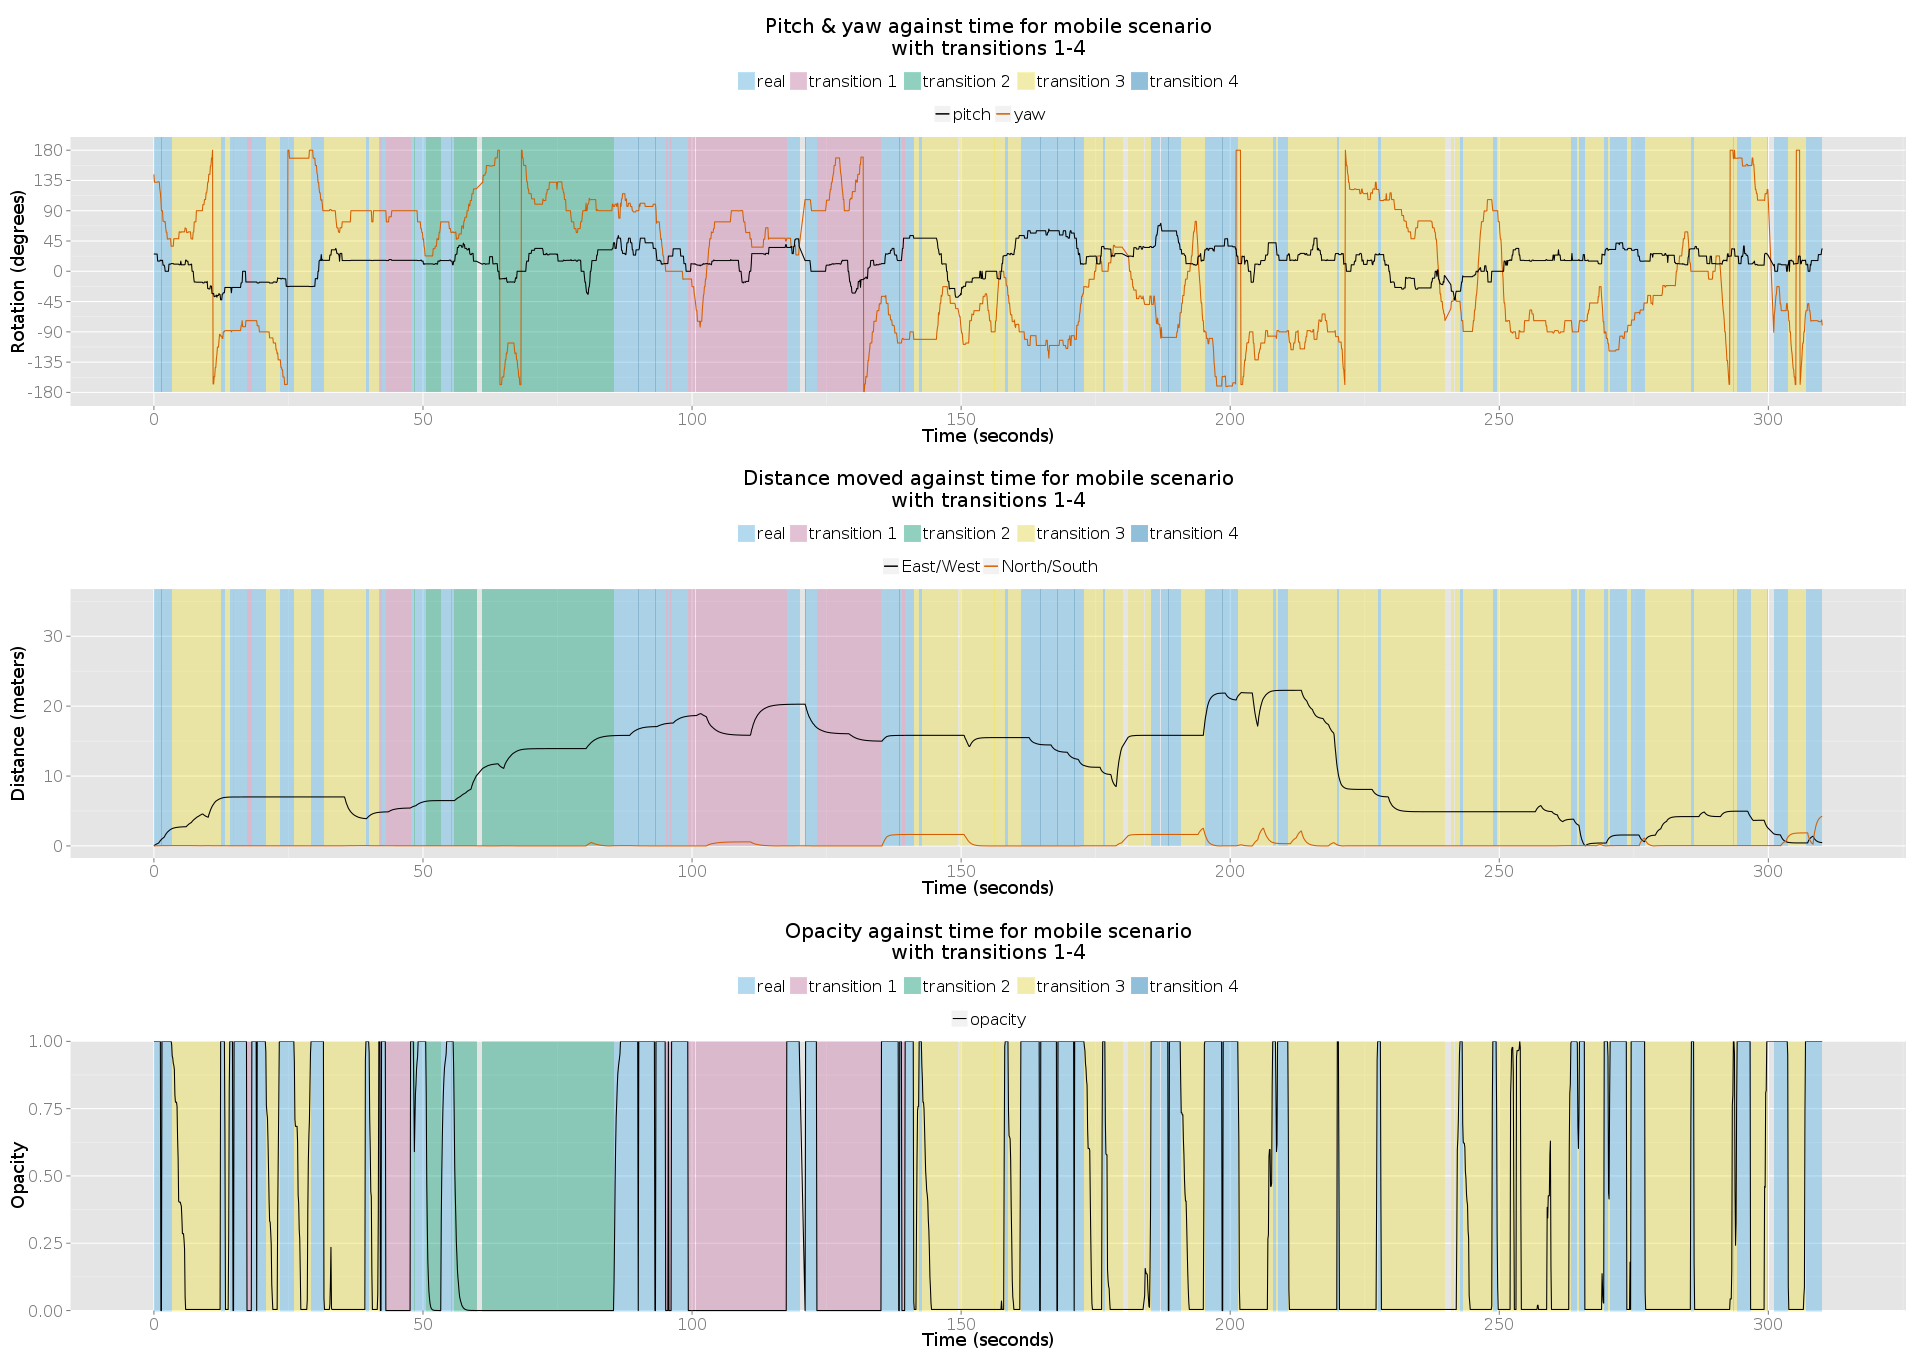
\includegraphics[width=\textwidth]{2.1/7_1-4_3up.png}
	\caption{Some images, yah.}
	\end{center}
\end{figure}

%=========================================================================================================

\clearpage

\subsection{Participant 8}

\begin{figure}[h]
	\begin{center}
	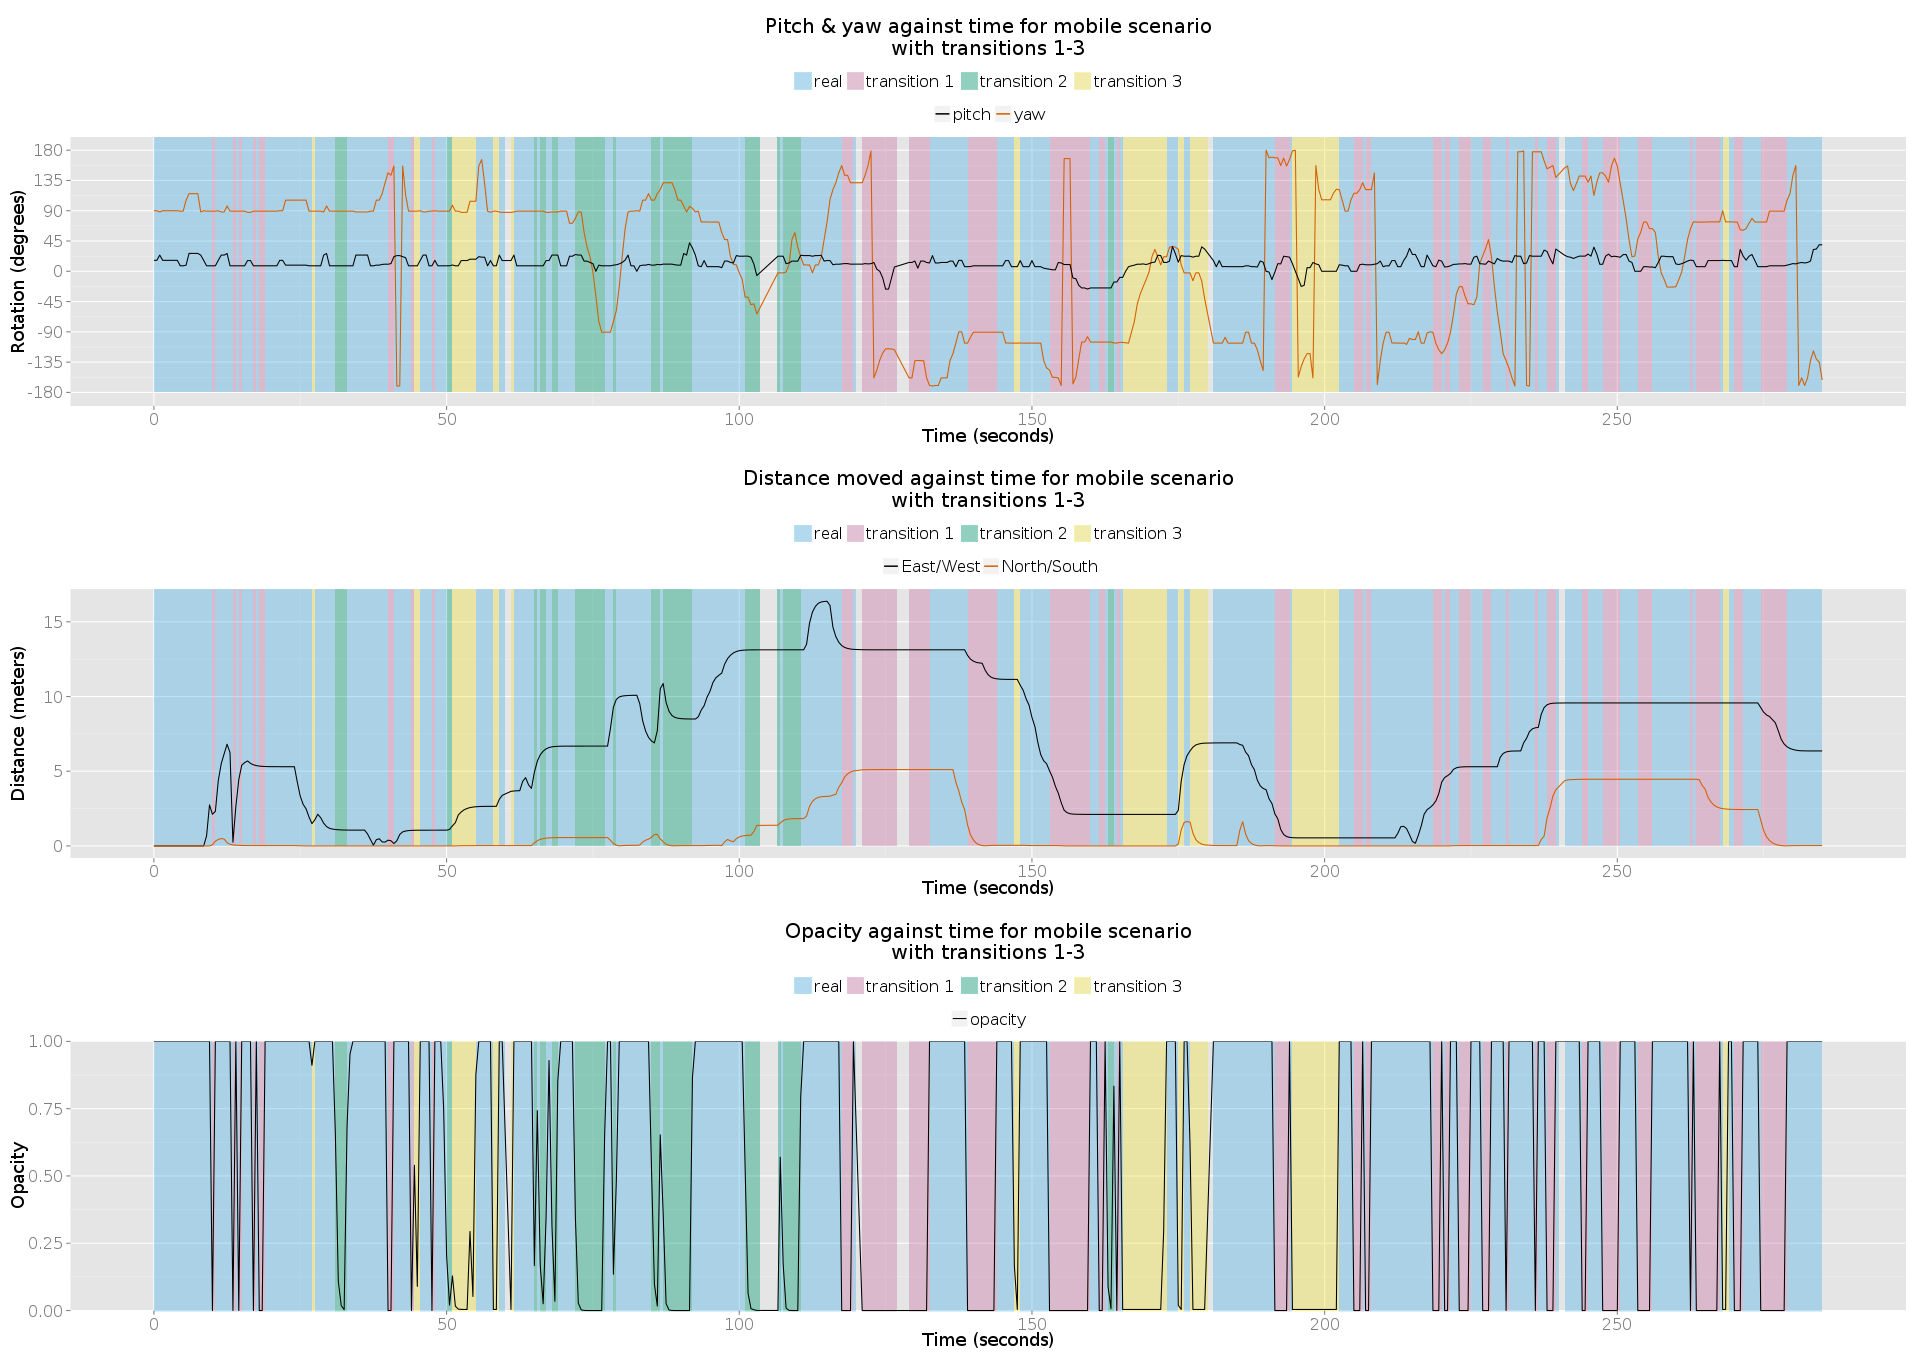
\includegraphics[width=\textwidth]{2.1/8_1-3_3up.png}
	\caption{Some images, yah.}
	\end{center}
\end{figure}

\clearpage

\begin{figure}[h]
	\begin{center}
	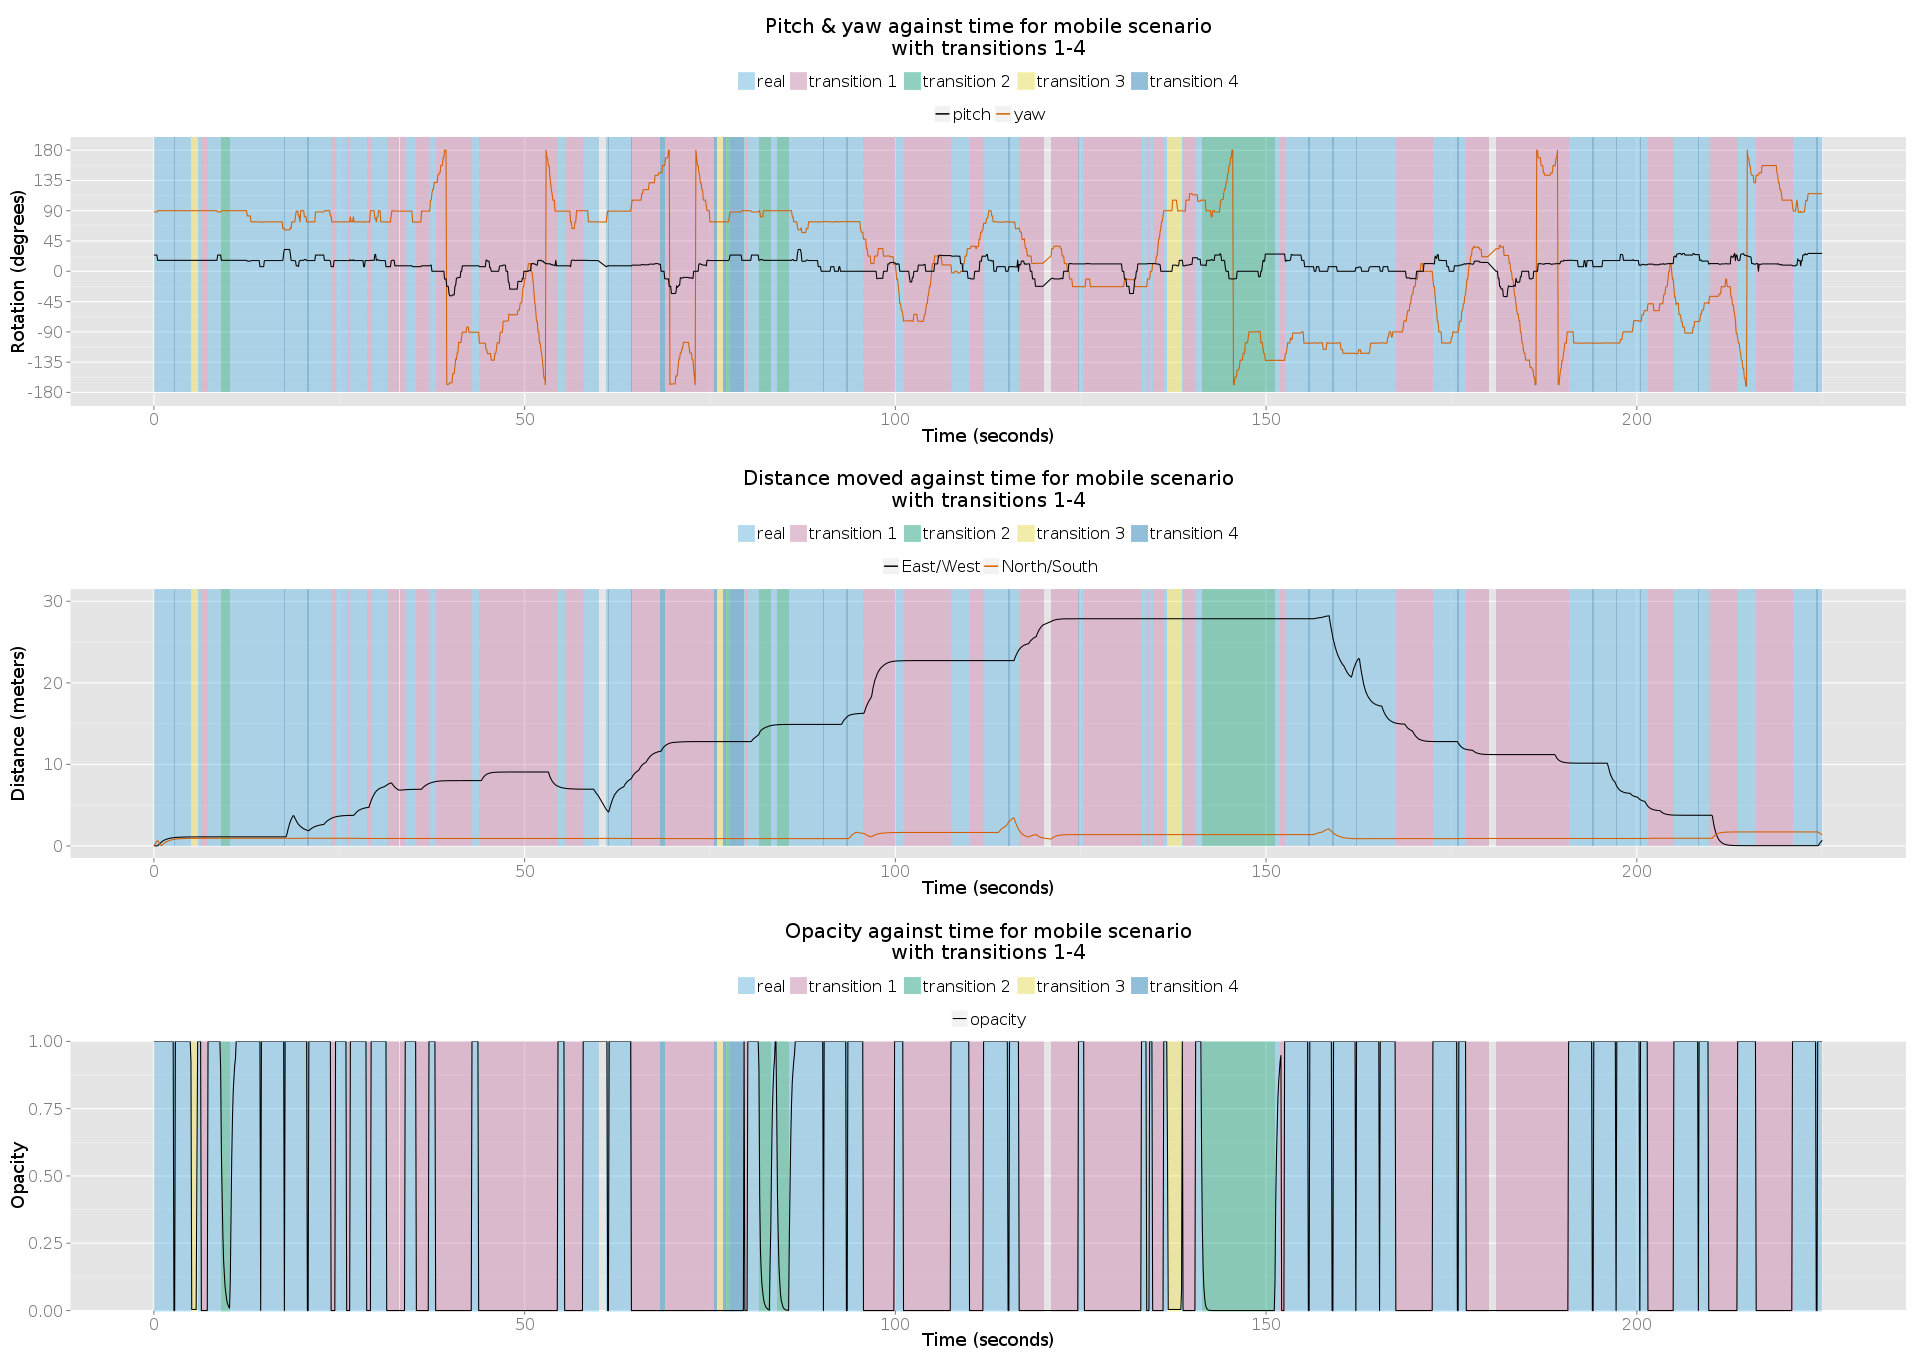
\includegraphics[width=\textwidth]{2.1/8_1-4_3up.png}
	\caption{Some images, yah.}
	\end{center}
\end{figure}

%=========================================================================================================

\clearpage

\subsection{Participant 9}

\begin{figure}[h]
	\begin{center}
	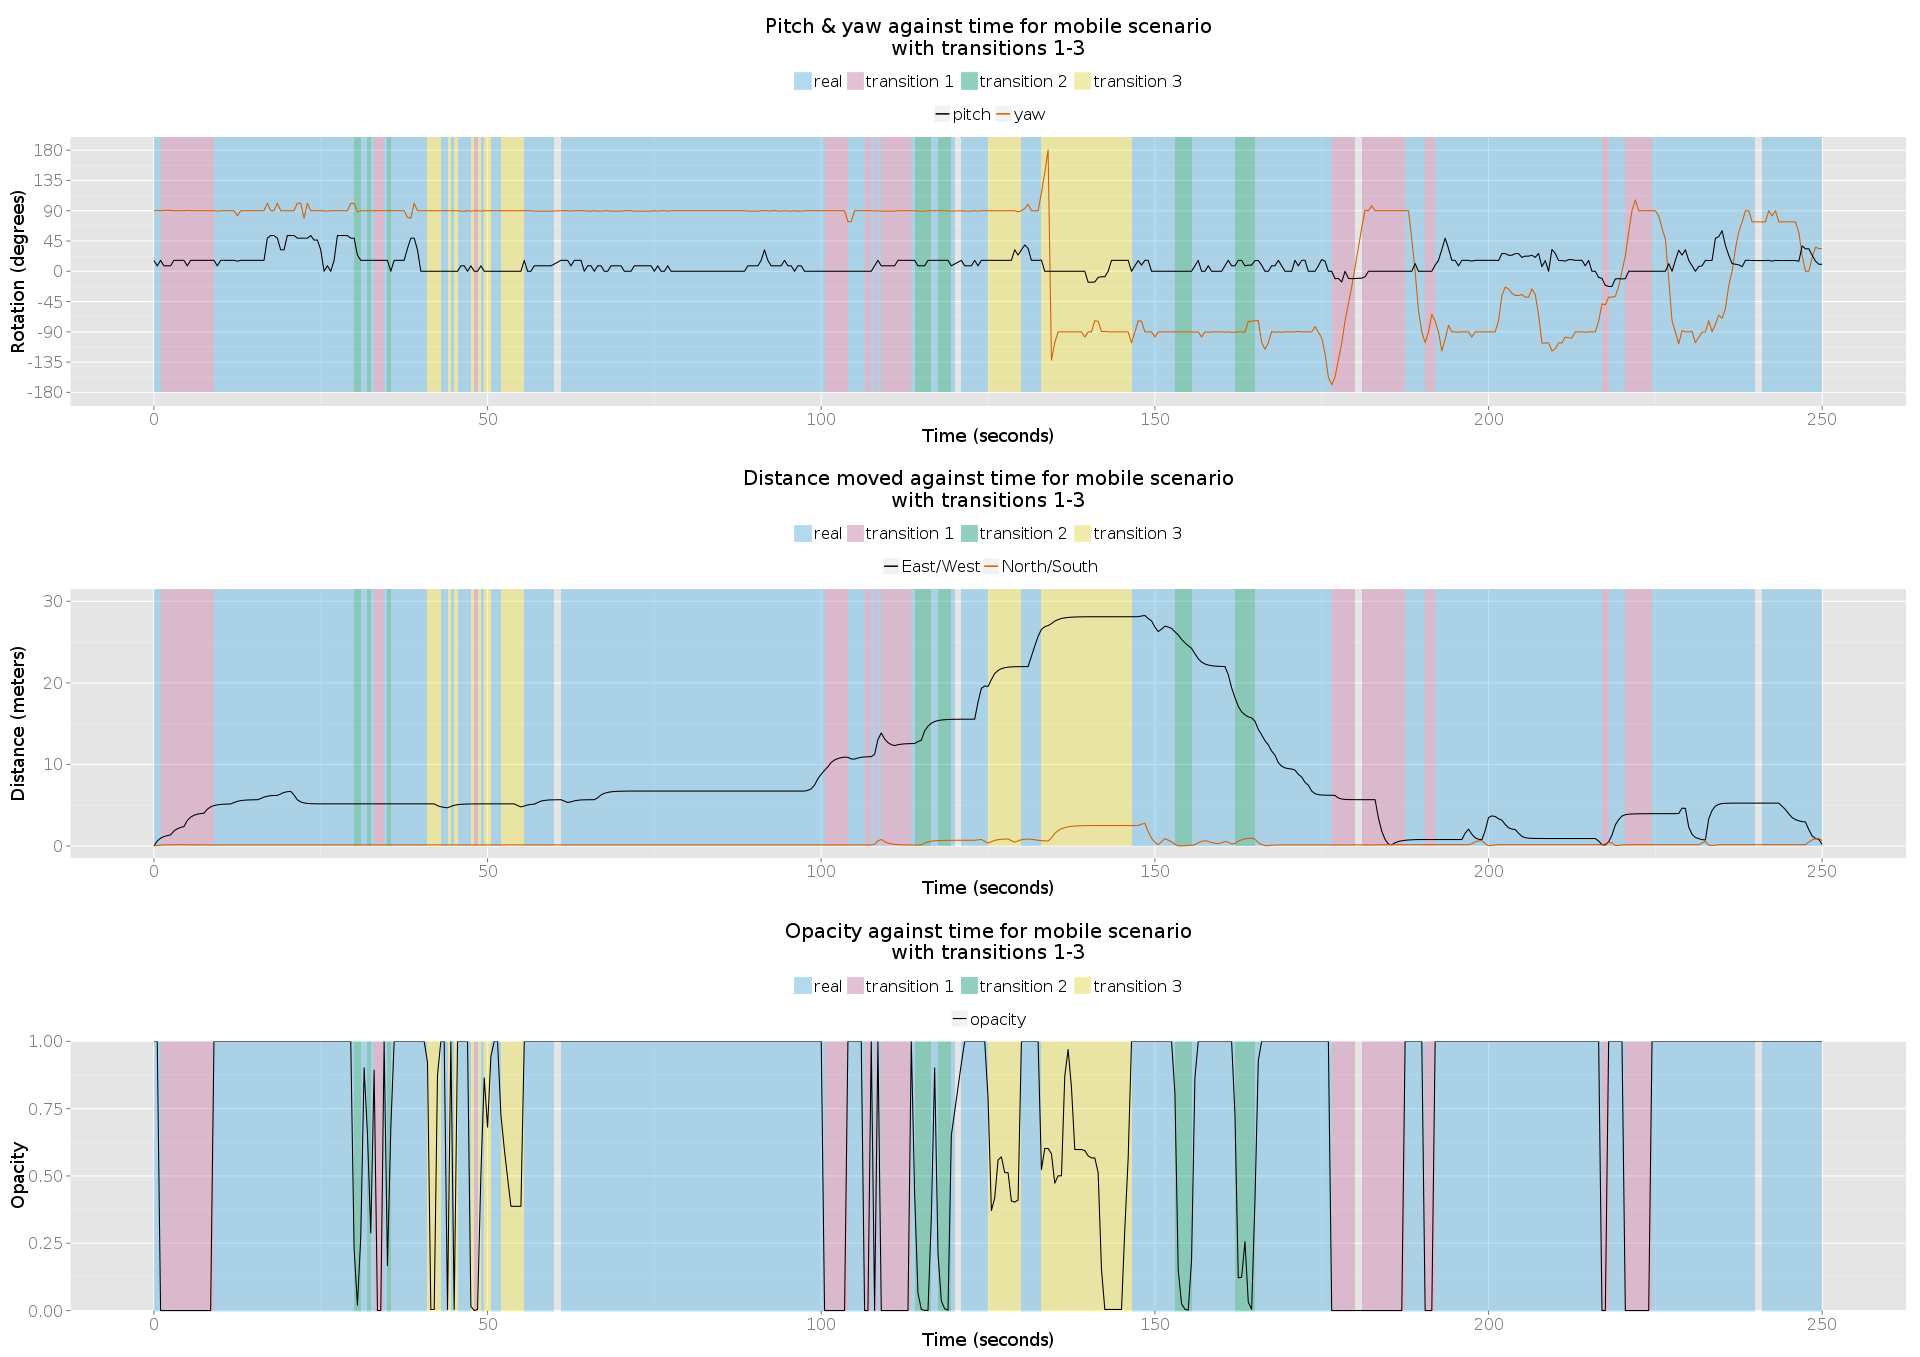
\includegraphics[width=\textwidth]{2.1/9_1-3_3up.png}
	\caption{Some images, yah.}
	\end{center}
\end{figure}

\clearpage

\begin{figure}[h]
	\begin{center}
	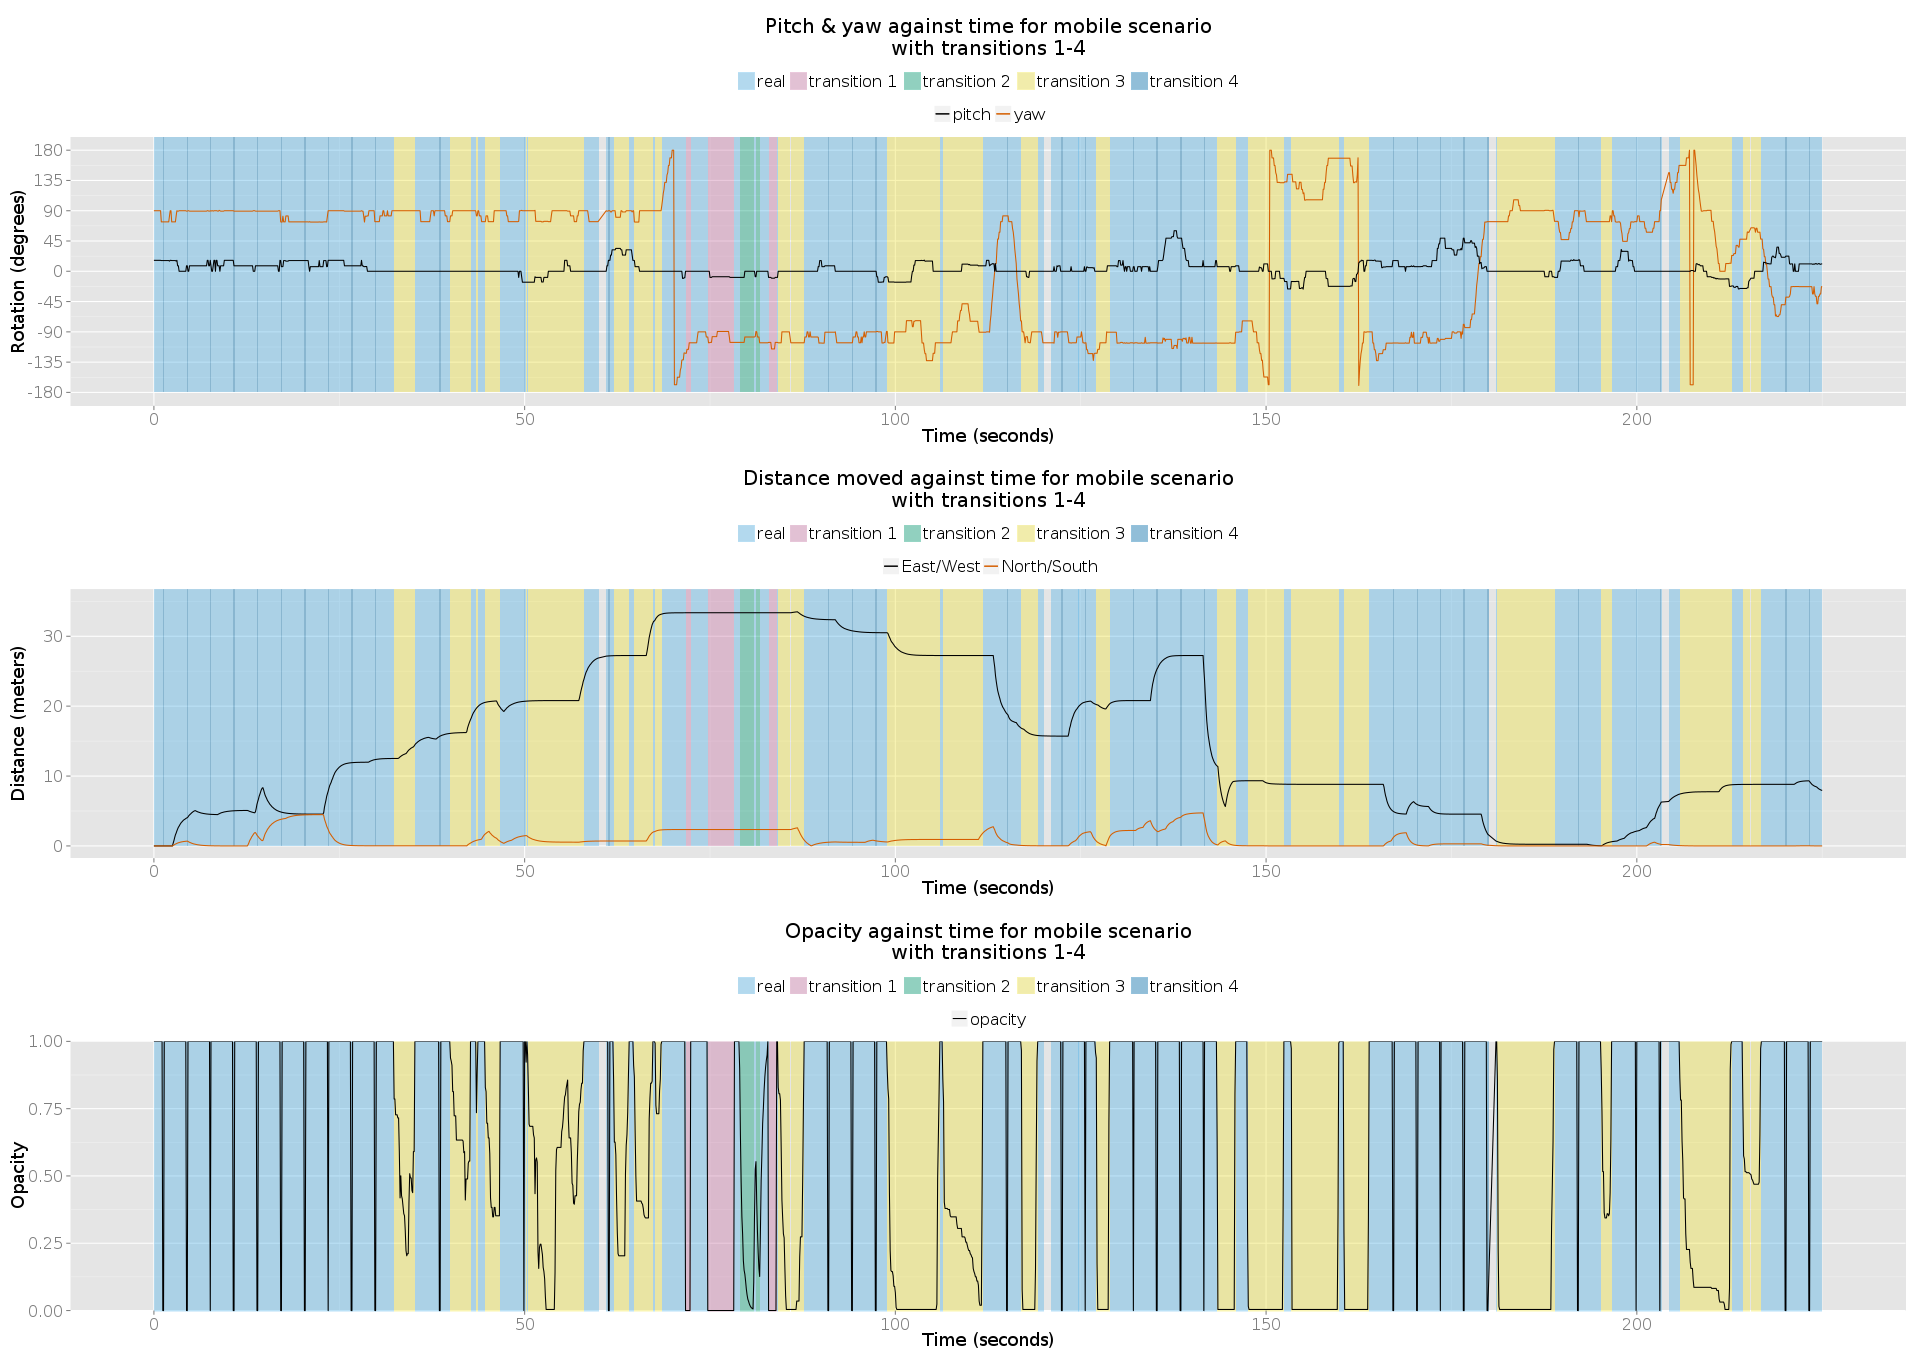
\includegraphics[width=\textwidth]{2.1/9_1-4_3up.png}
	\caption{Some images, yah.}
	\end{center}
\end{figure}

%=========================================================================================================

\clearpage

\subsection{Participant 10}

\begin{figure}[h]
	\begin{center}
	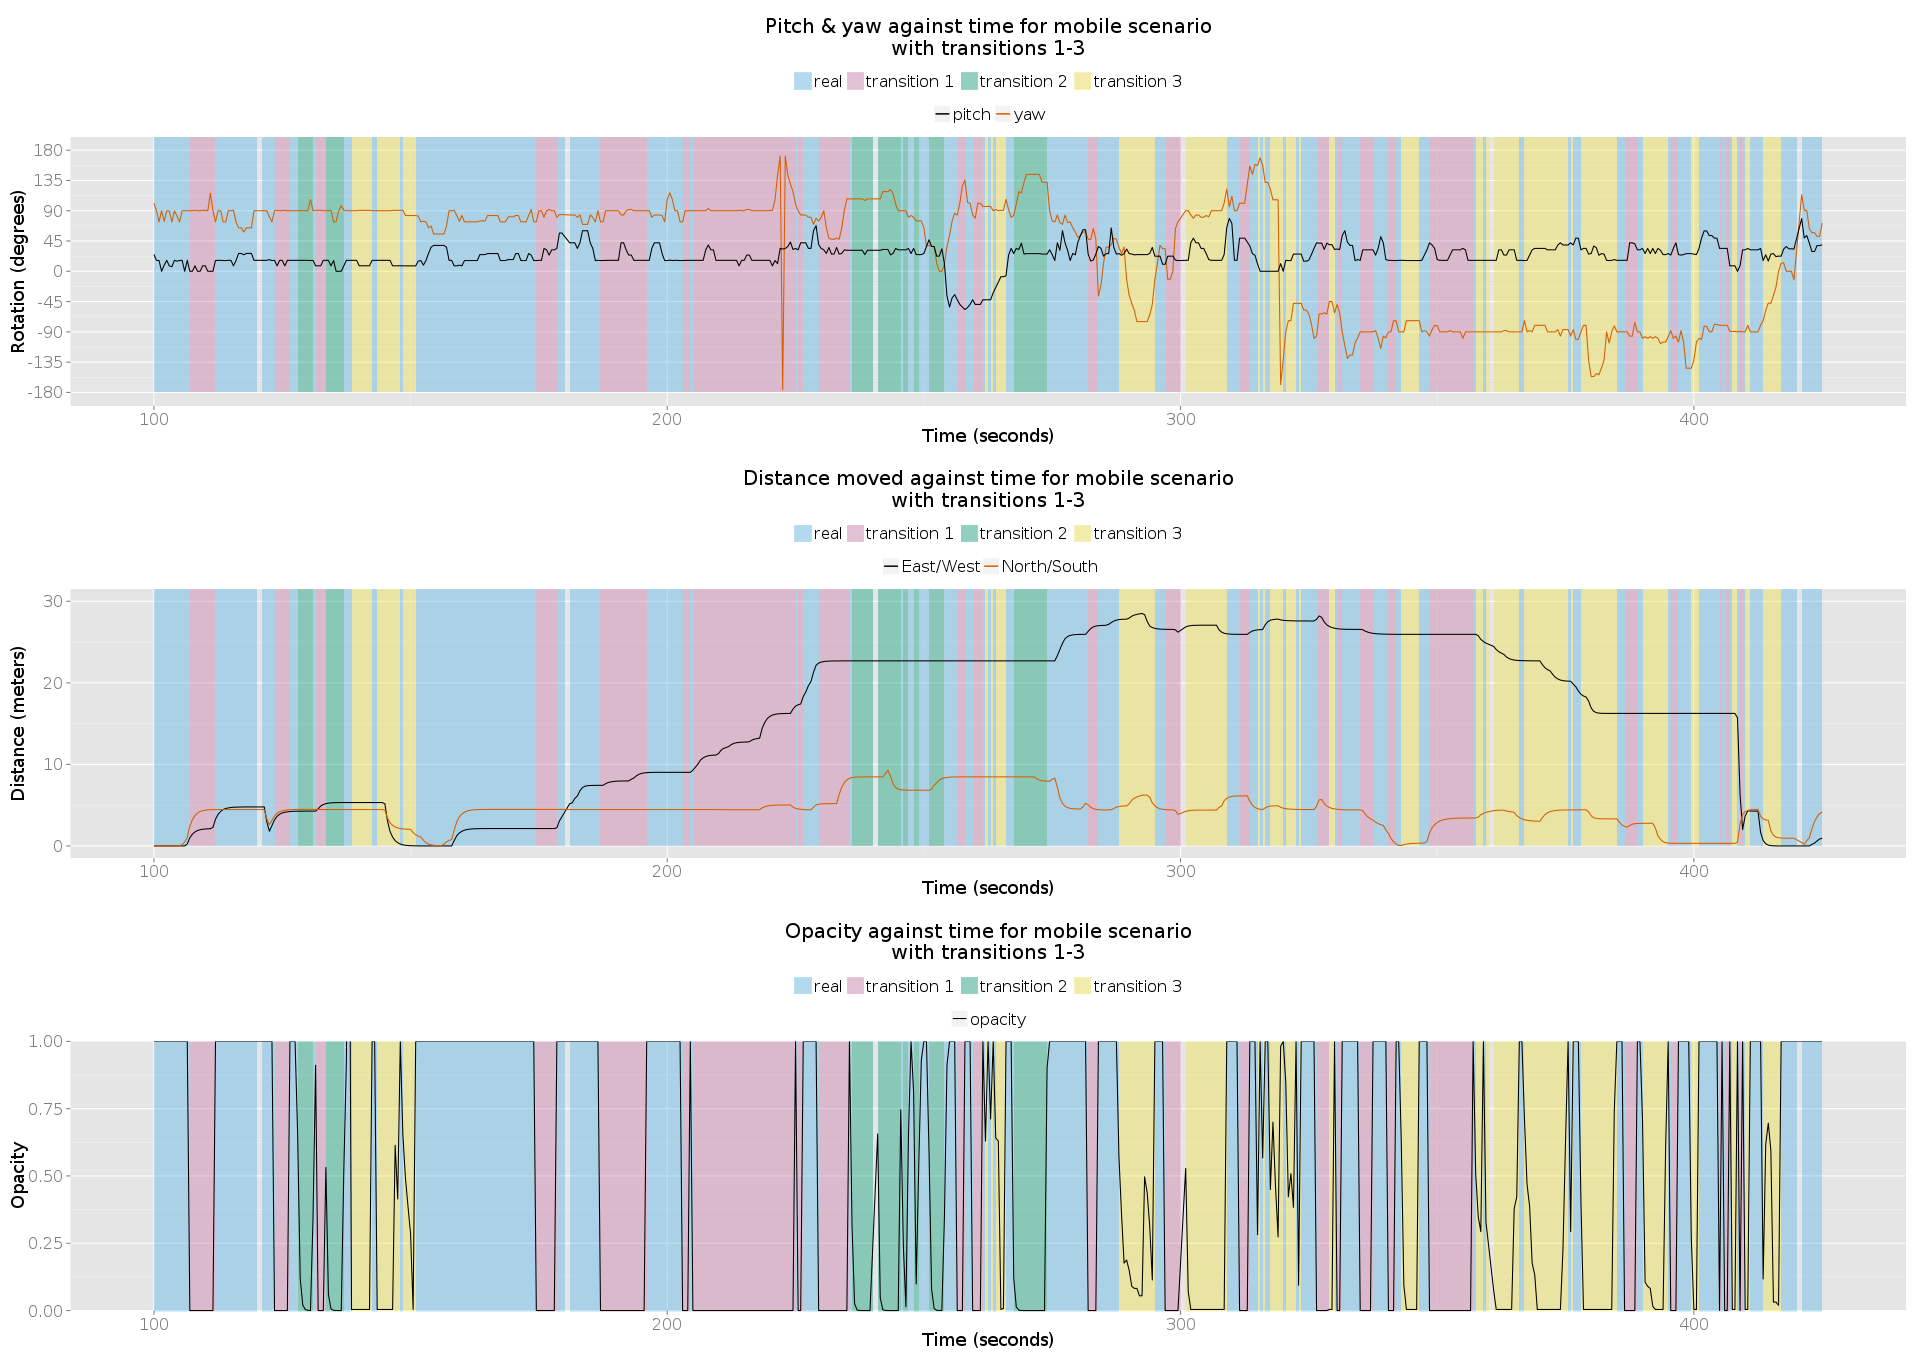
\includegraphics[width=\textwidth]{2.1/10_1-3_3up.png}
	\caption{Some images, yah.}
	\end{center}
\end{figure}

\clearpage

\begin{figure}[h]
	\begin{center}
	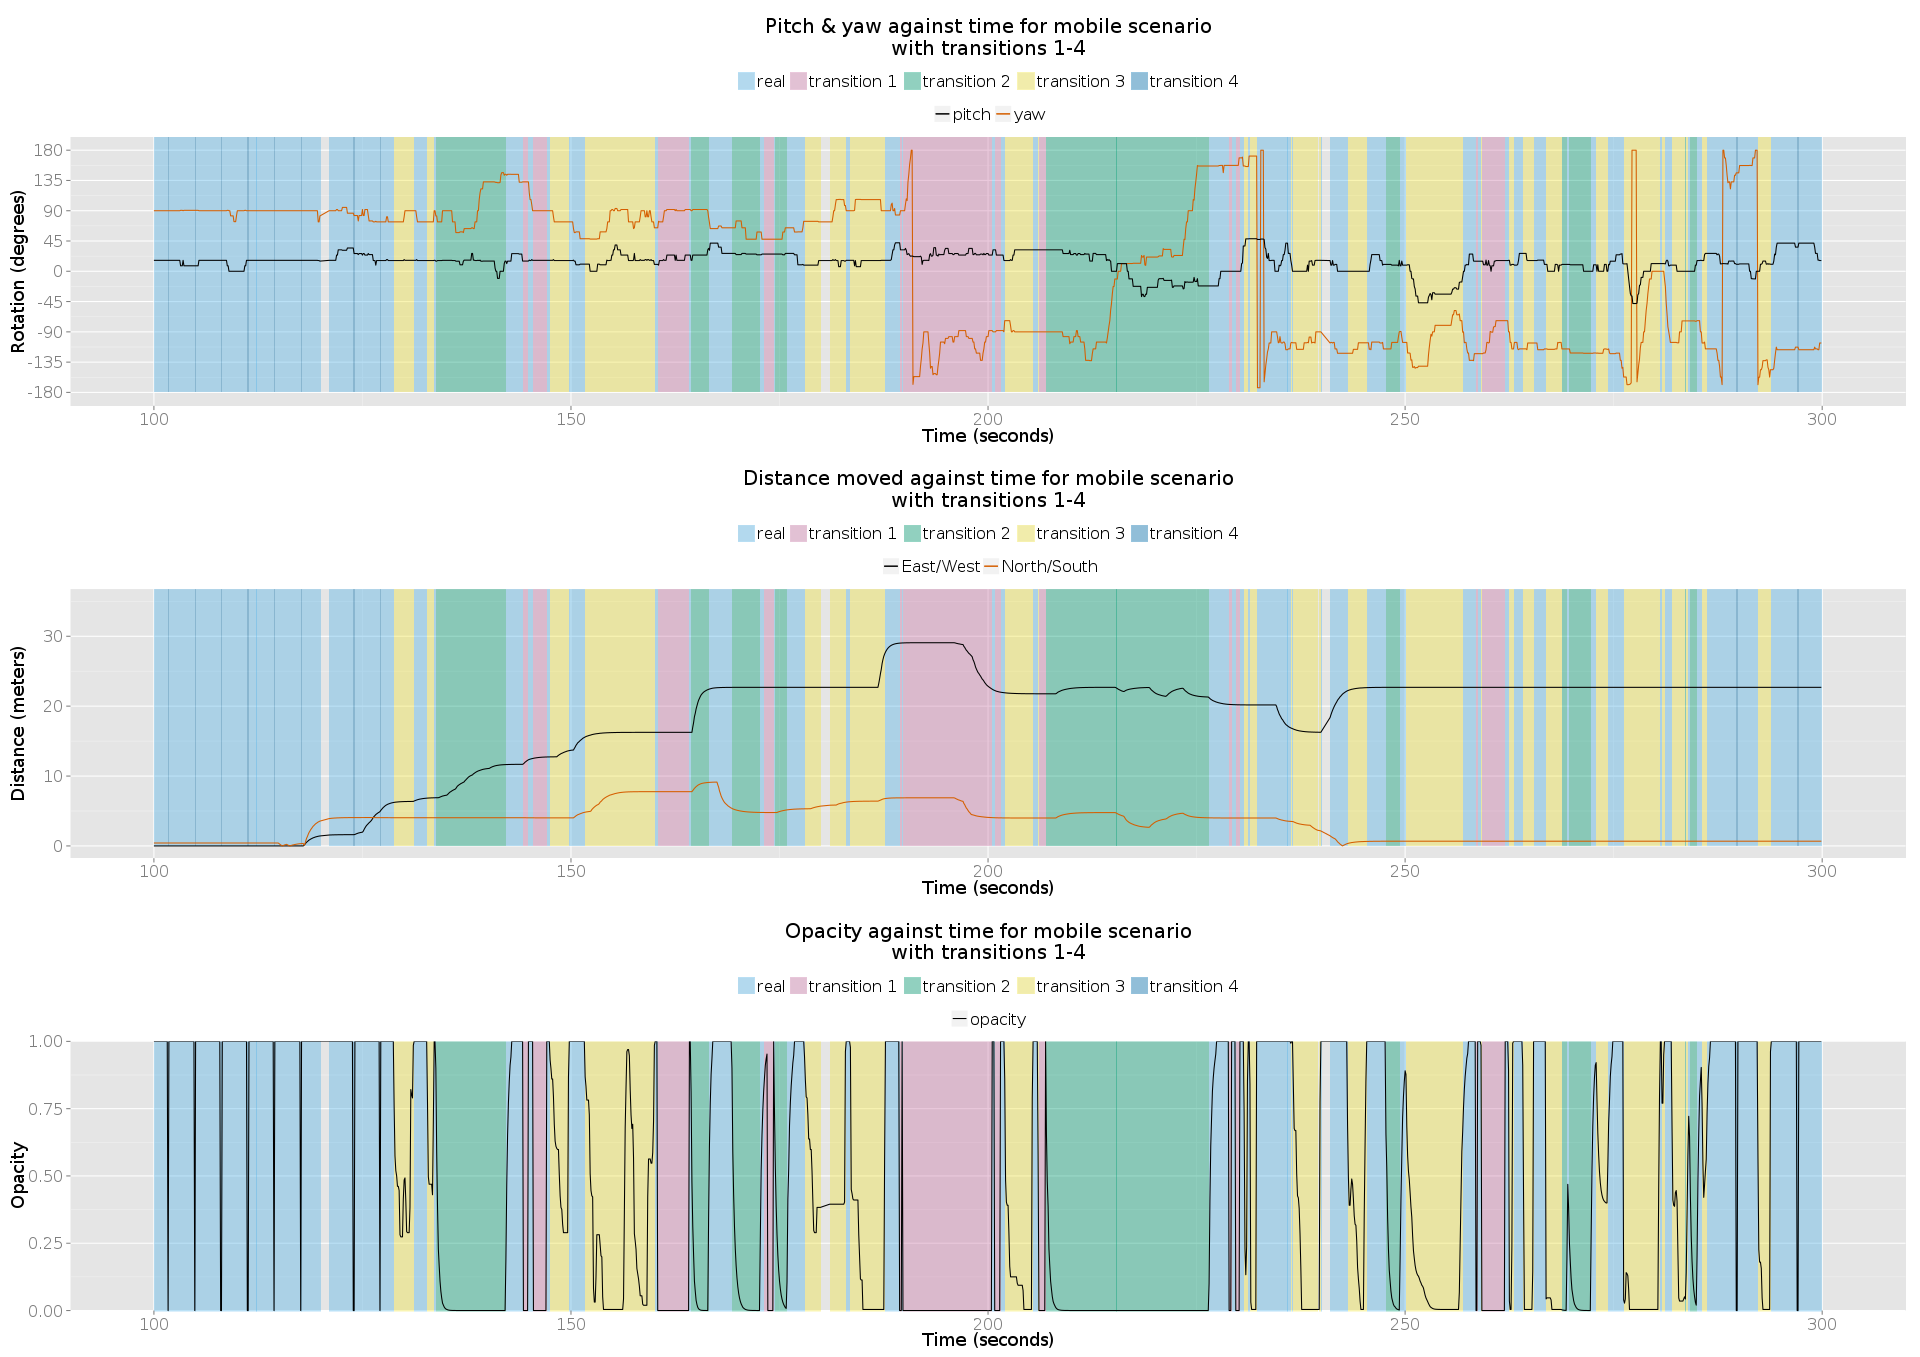
\includegraphics[width=\textwidth]{2.1/10_1-4_3up.png}
	\caption{Some images, yah.}
	\end{center}
\end{figure}

%=========================================================================================================

\clearpage

\subsection{Participant 11}

\begin{figure}[h]
	\begin{center}
	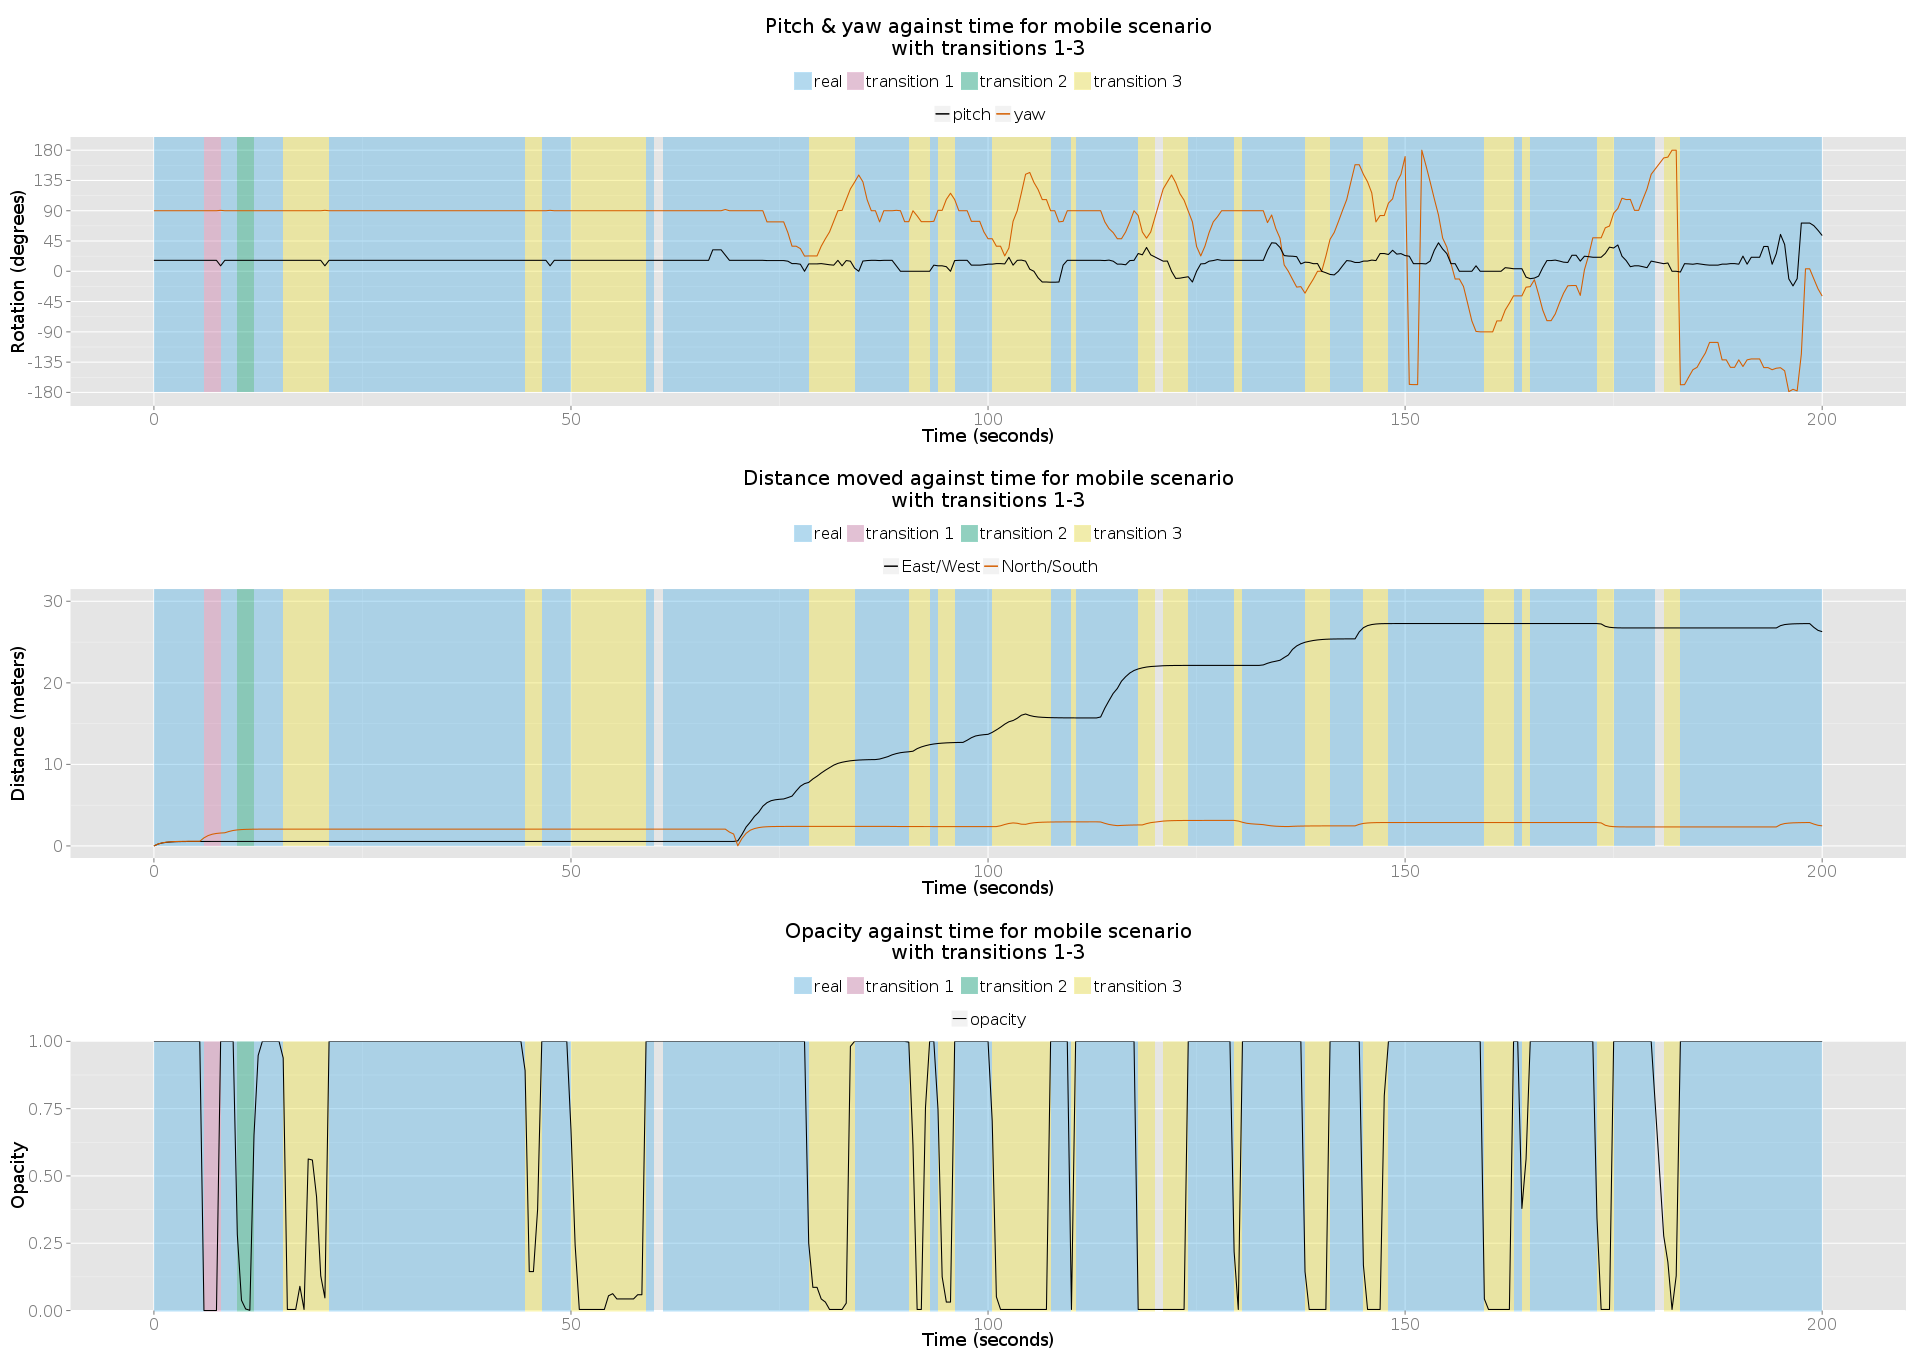
\includegraphics[width=\textwidth]{2.1/11_1-3_3up.png}
	\caption{Some images, yah.}
	\end{center}
\end{figure}

\clearpage

\begin{figure}[h]
	\begin{center}
	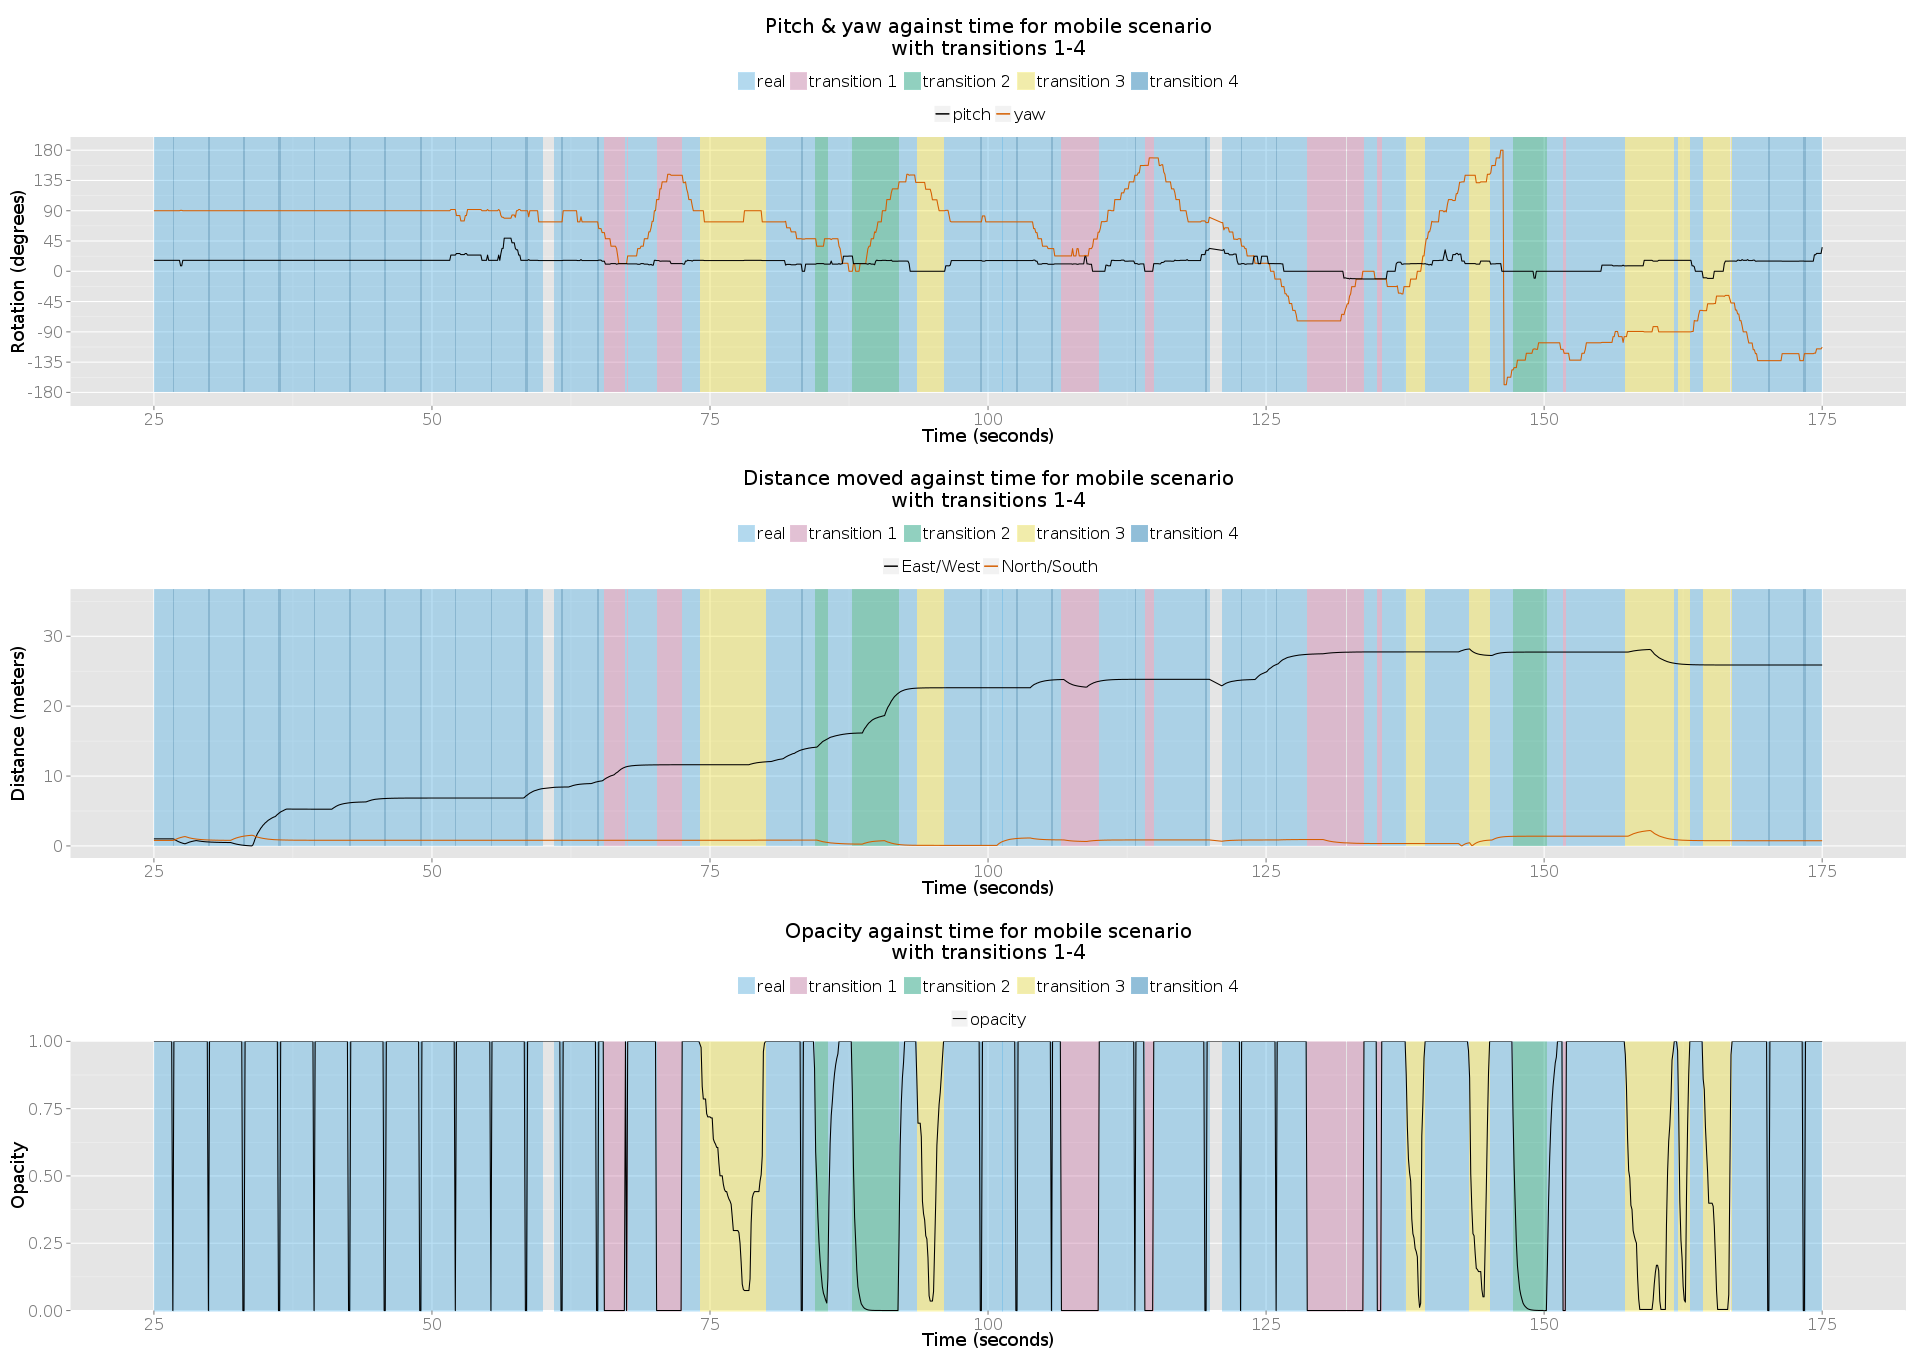
\includegraphics[width=\textwidth]{2.1/11_1-4_3up.png}
	\caption{Some images, yah.}
	\end{center}
\end{figure}

%=========================================================================================================

\clearpage

\subsection{Participant 12}

\begin{figure}[h]
	\begin{center}
	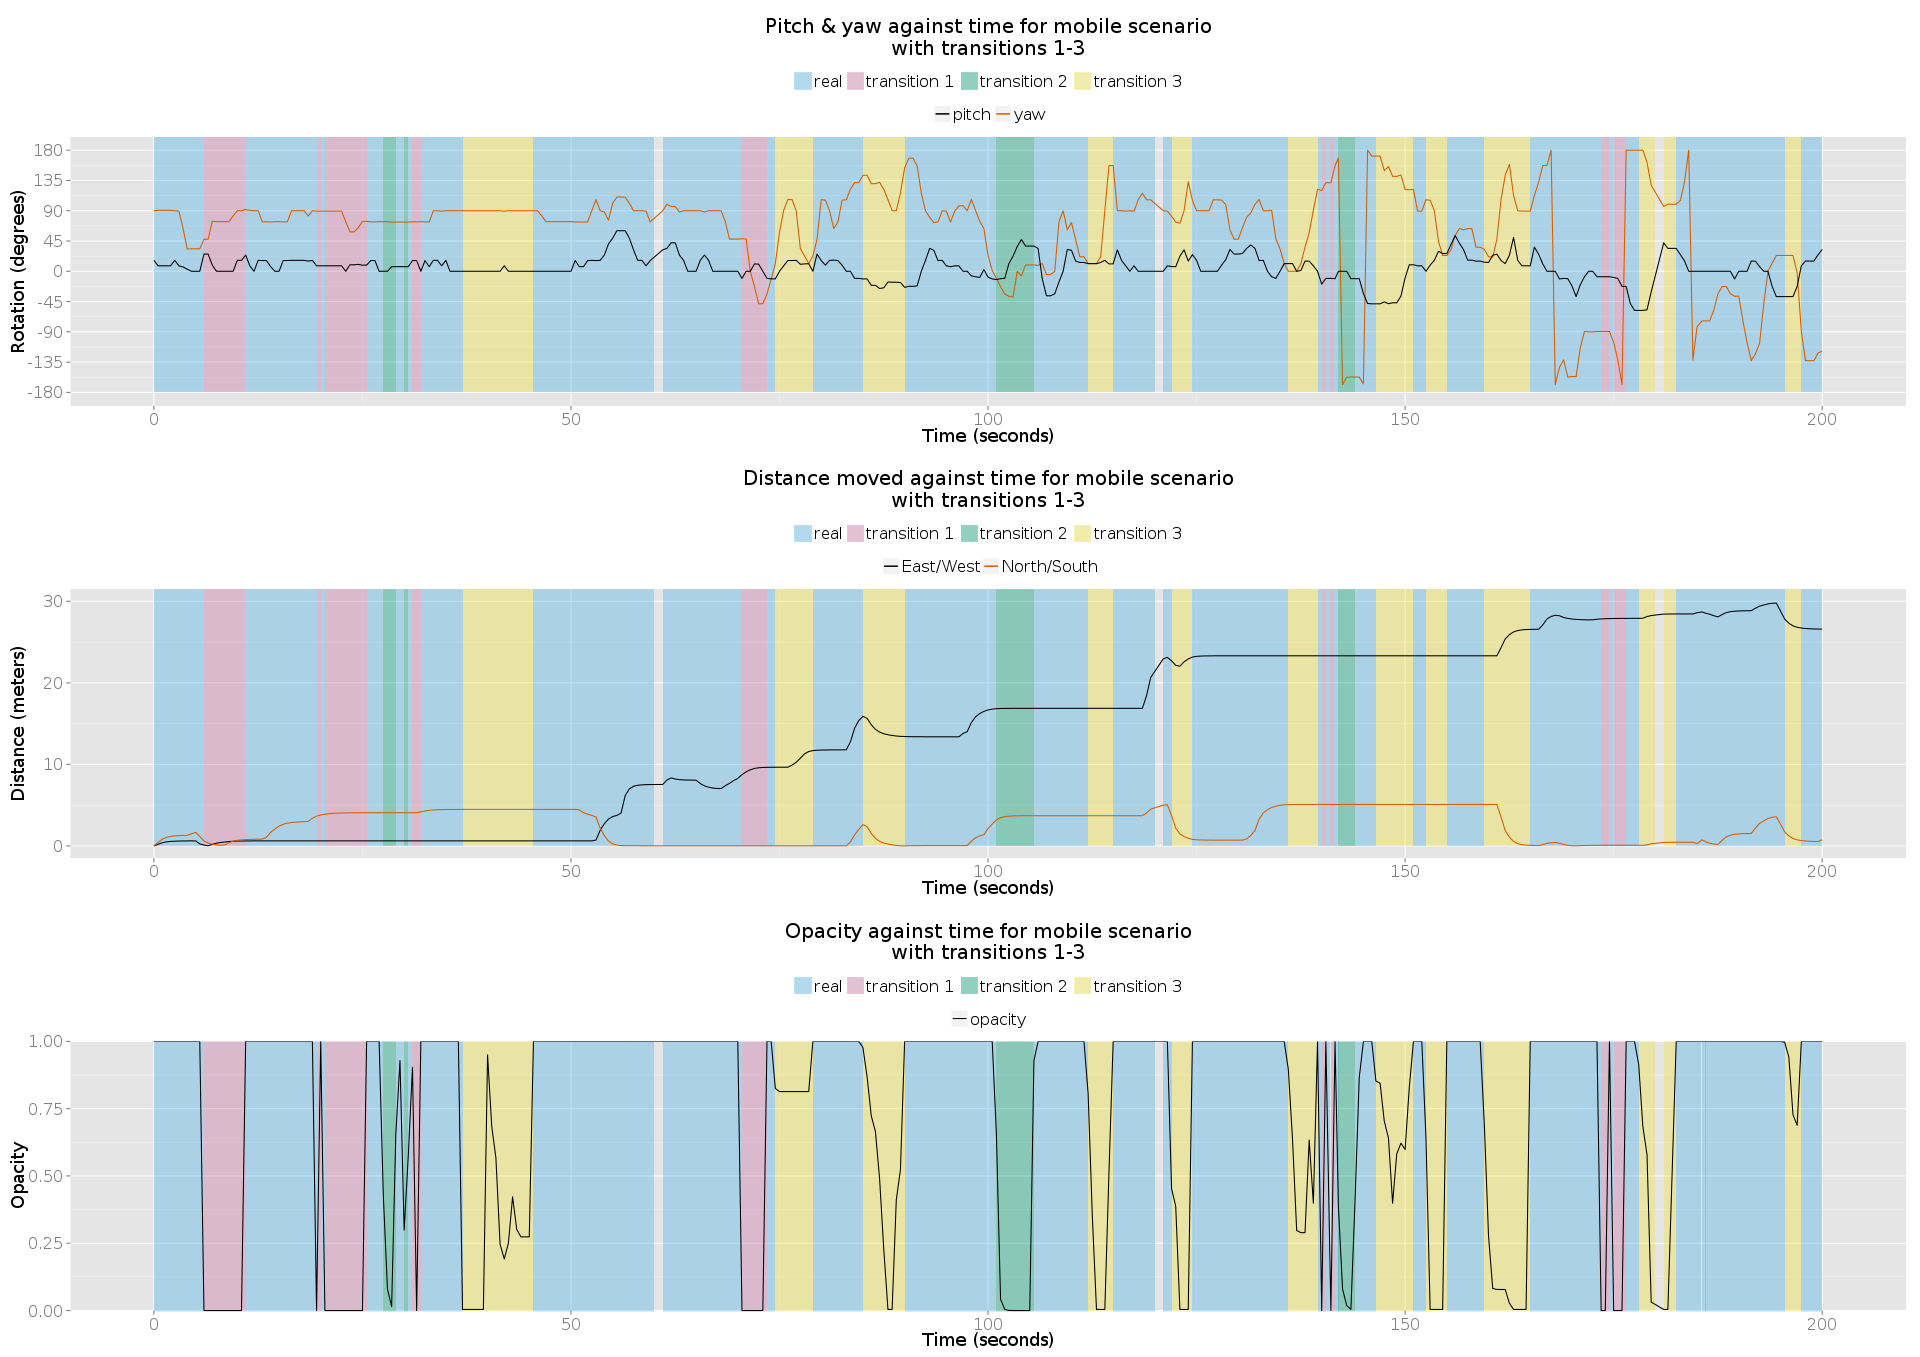
\includegraphics[width=\textwidth]{2.1/12_1-3_3up.png}
	\caption{Some images, yah.}
	\end{center}
\end{figure}

\clearpage

\begin{figure}[h]
	\begin{center}
	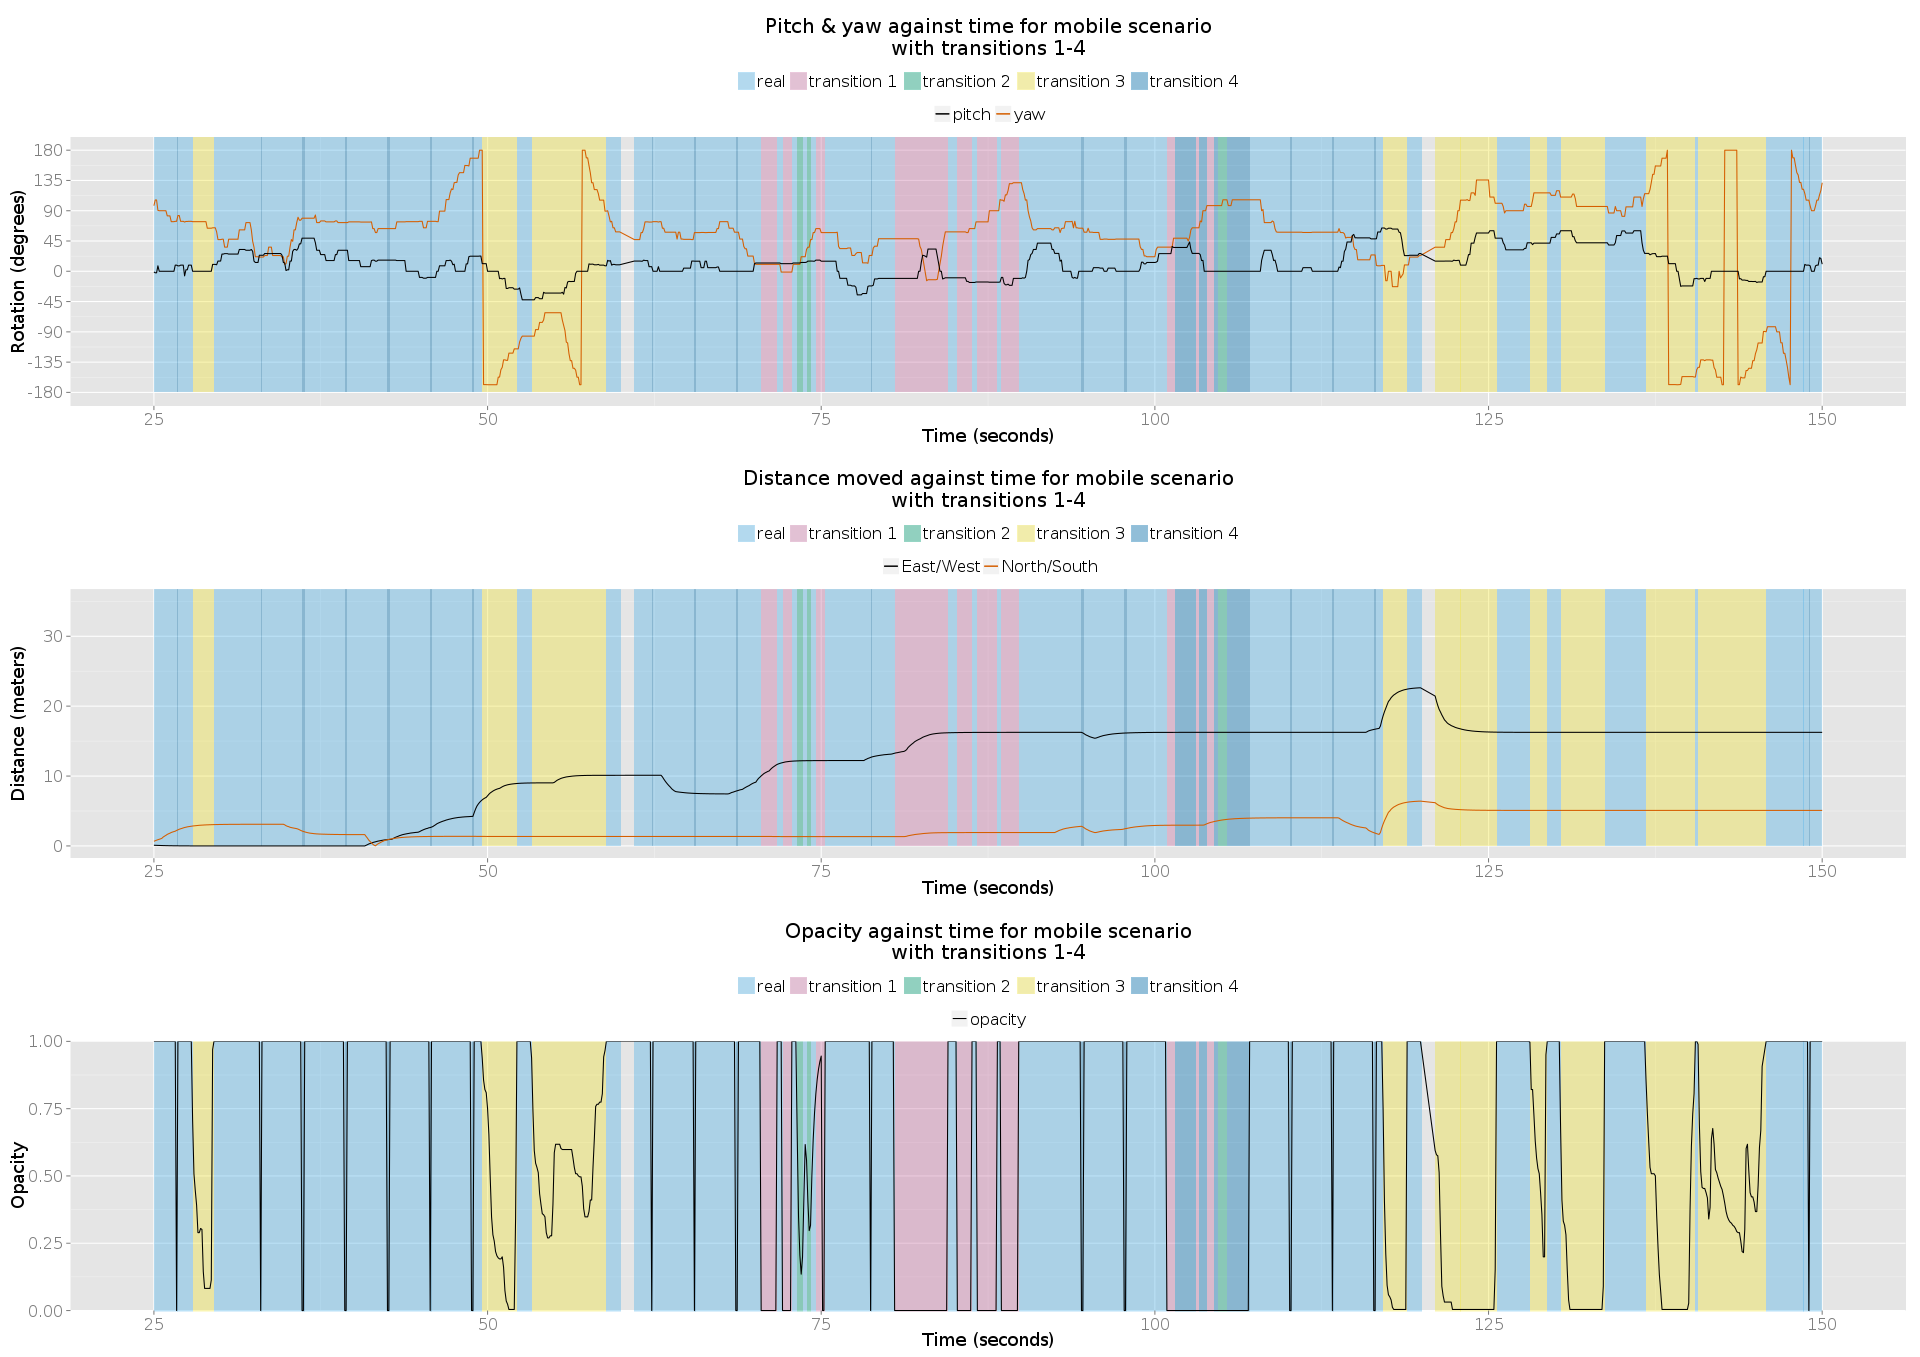
\includegraphics[width=\textwidth]{2.1/12_1-4_3up.png}
	\caption{Some images, yah.}
	\end{center}
\end{figure}

%=========================================================================================================

\clearpage

\subsection{Participant 13}

\begin{figure}[h]
	\begin{center}
	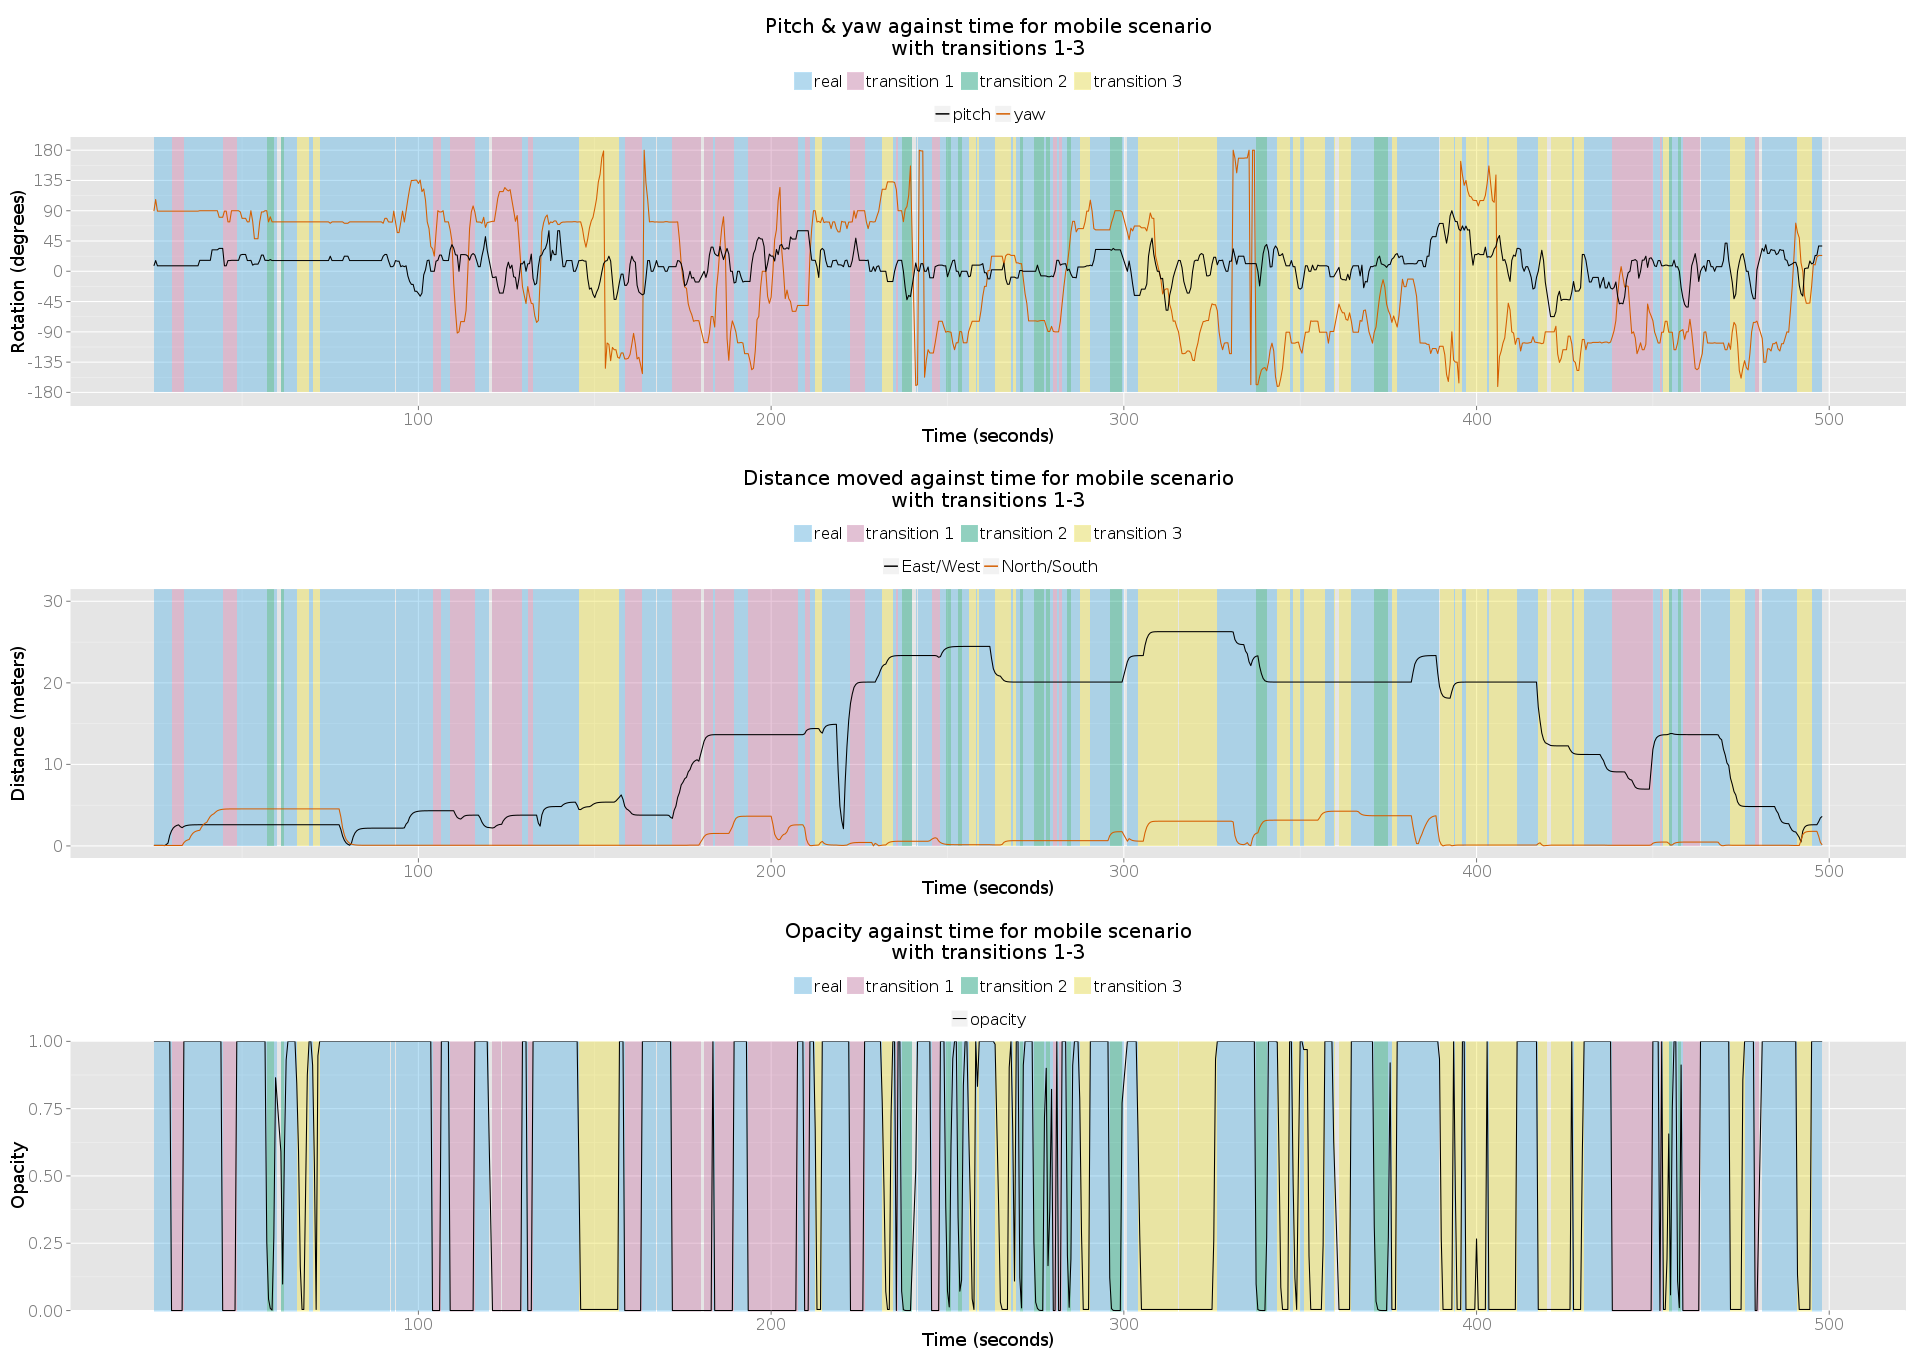
\includegraphics[width=\textwidth]{2.1/13_1-3_3up.png}
	\caption{Some images, yah.}
	\end{center}
\end{figure}

\clearpage

\begin{figure}[h]
	\begin{center}
	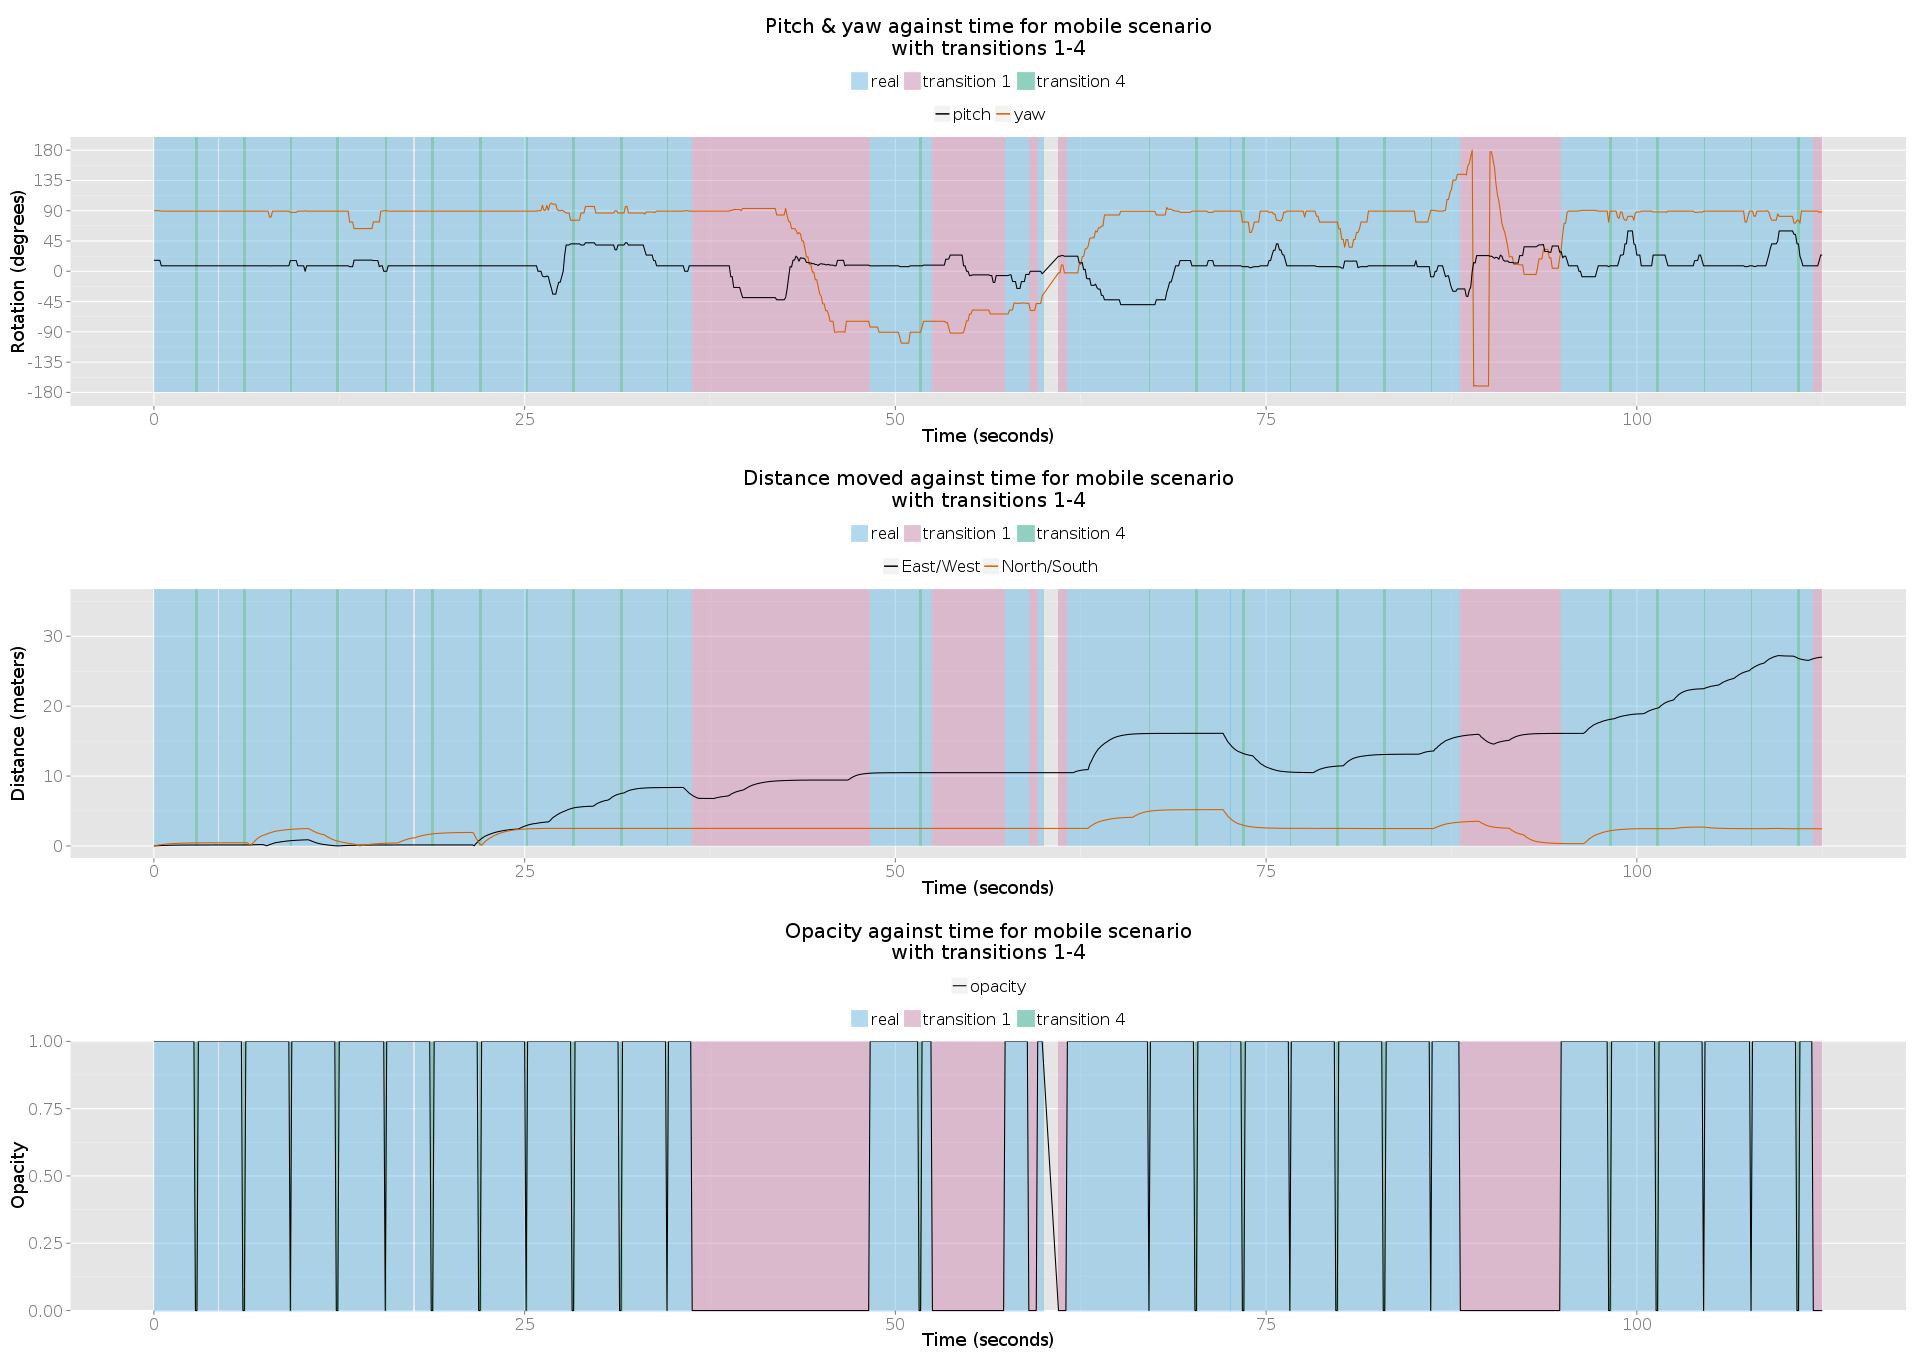
\includegraphics[width=\textwidth]{2.1/13_1-4_3up.png}
	\caption{Some images, yah.}
	\end{center}
\end{figure}

%=========================================================================================================

\clearpage

\section{Phase 2.2 Results}

%=========================================================================================================

\clearpage

\subsection{Participant 14}

\begin{figure}[h]
	\begin{center}
	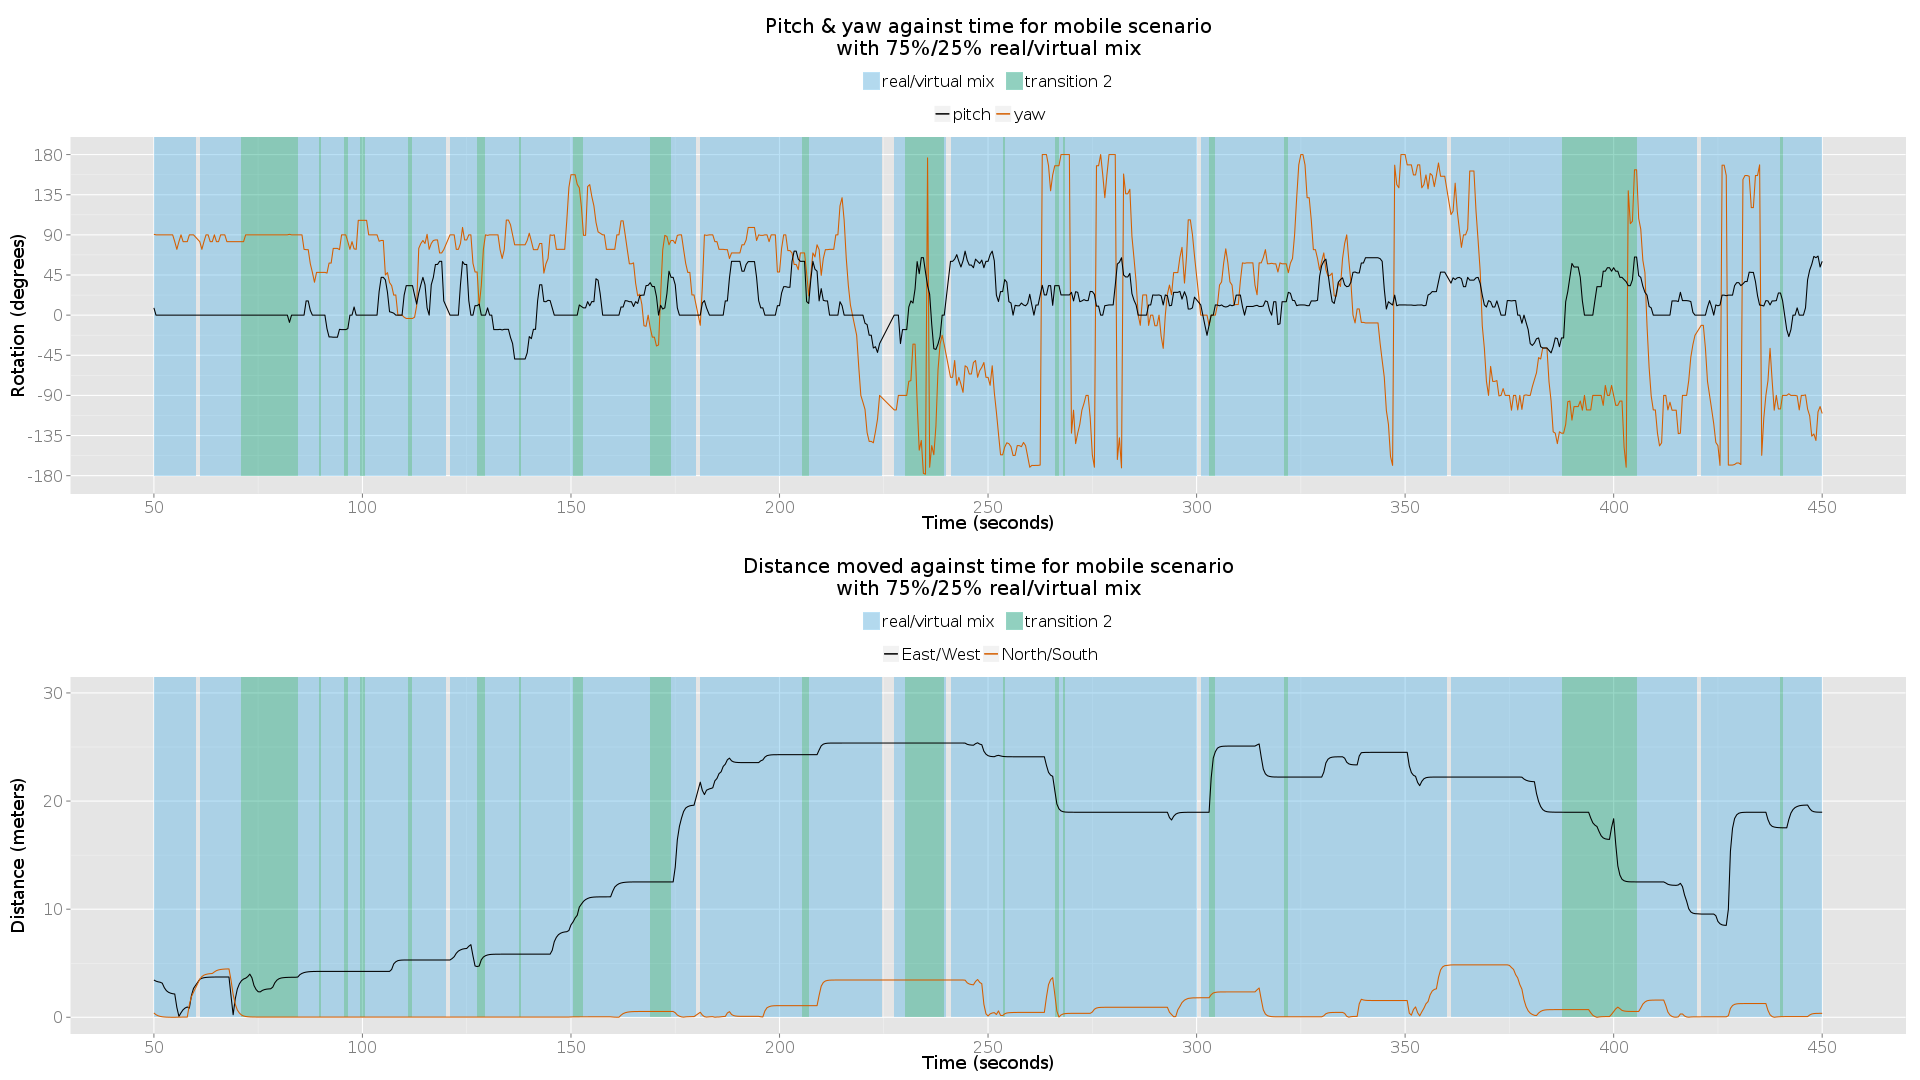
\includegraphics[width=\textwidth]{2.2/14_75_2up.png}
	\caption{Some images, yah.}
	\end{center}
\end{figure}

\clearpage

\begin{figure}[h]
	\begin{center}
	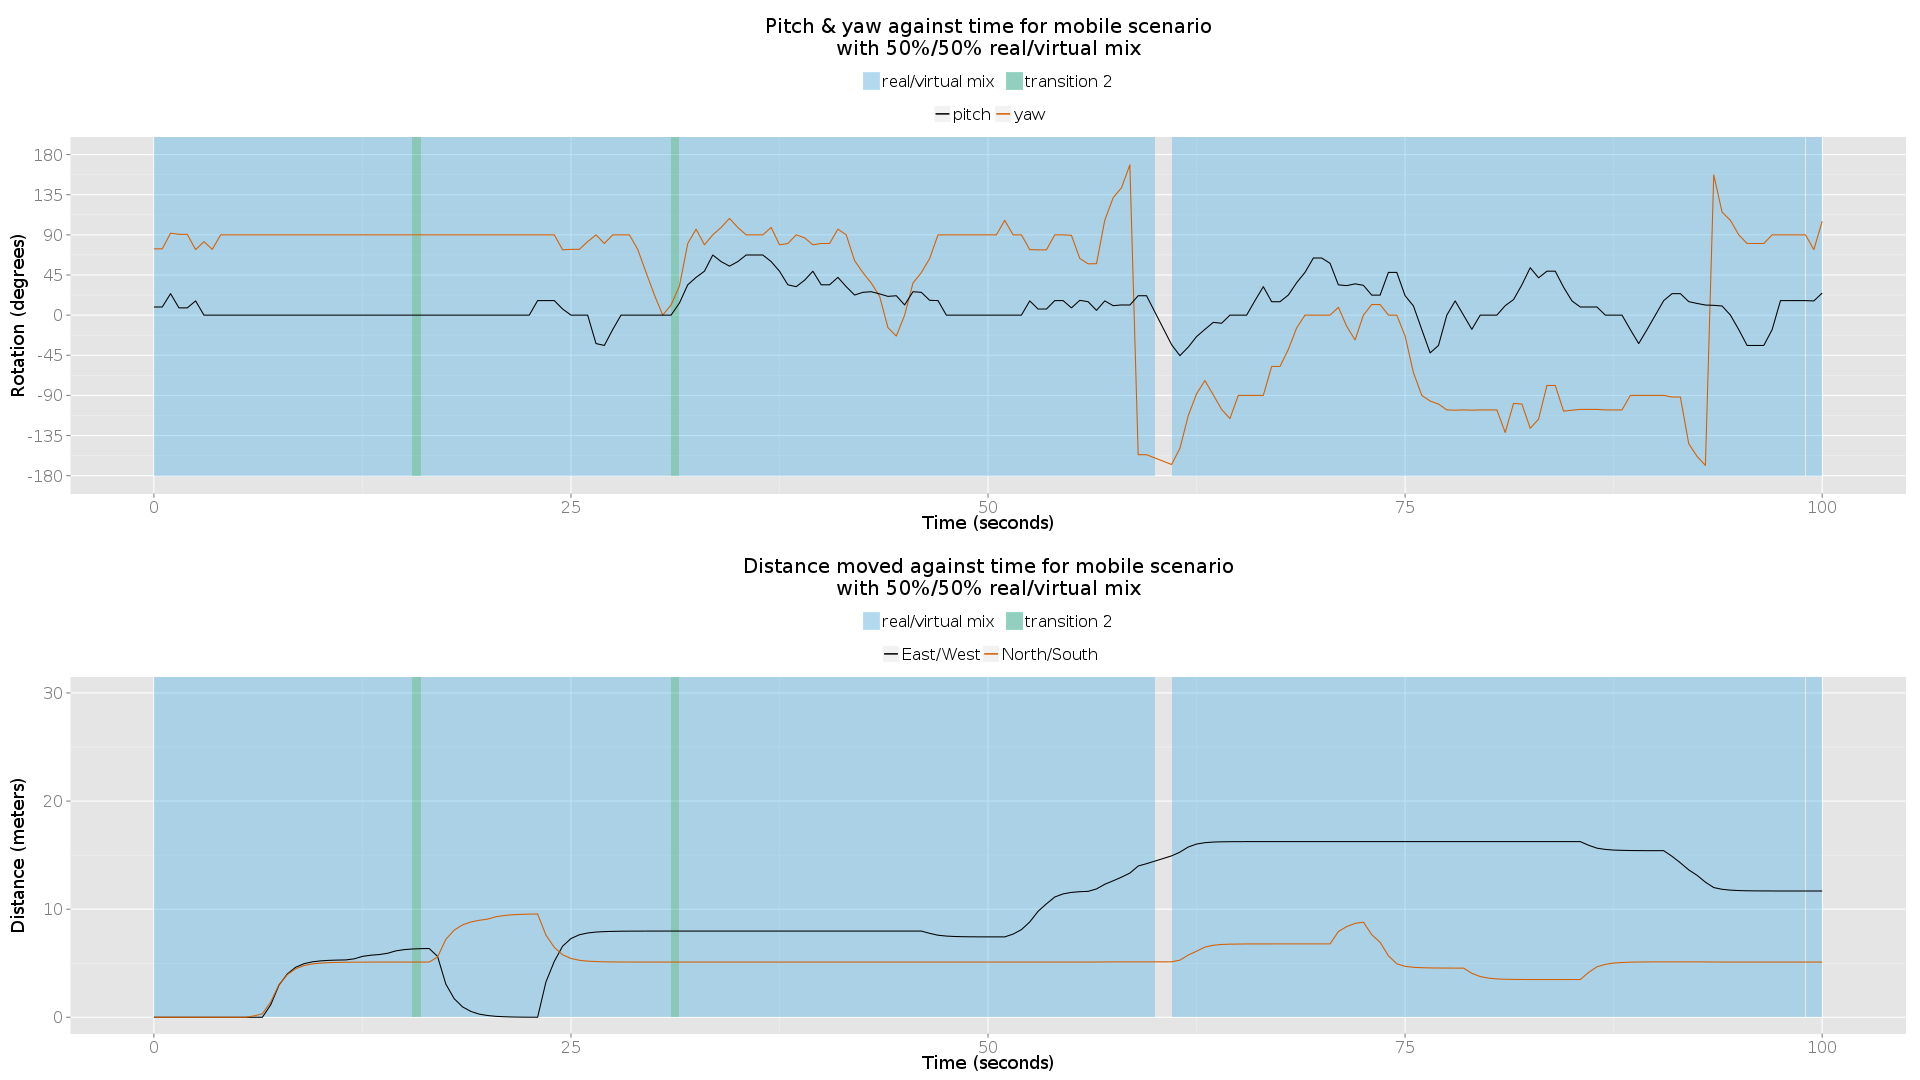
\includegraphics[width=\textwidth]{2.2/14_50_2up.png}
	\caption{Some images, yah.}
	\end{center}
\end{figure}

%=========================================================================================================

\clearpage

\subsection{Participant 15}

\begin{figure}[h]
	\begin{center}
	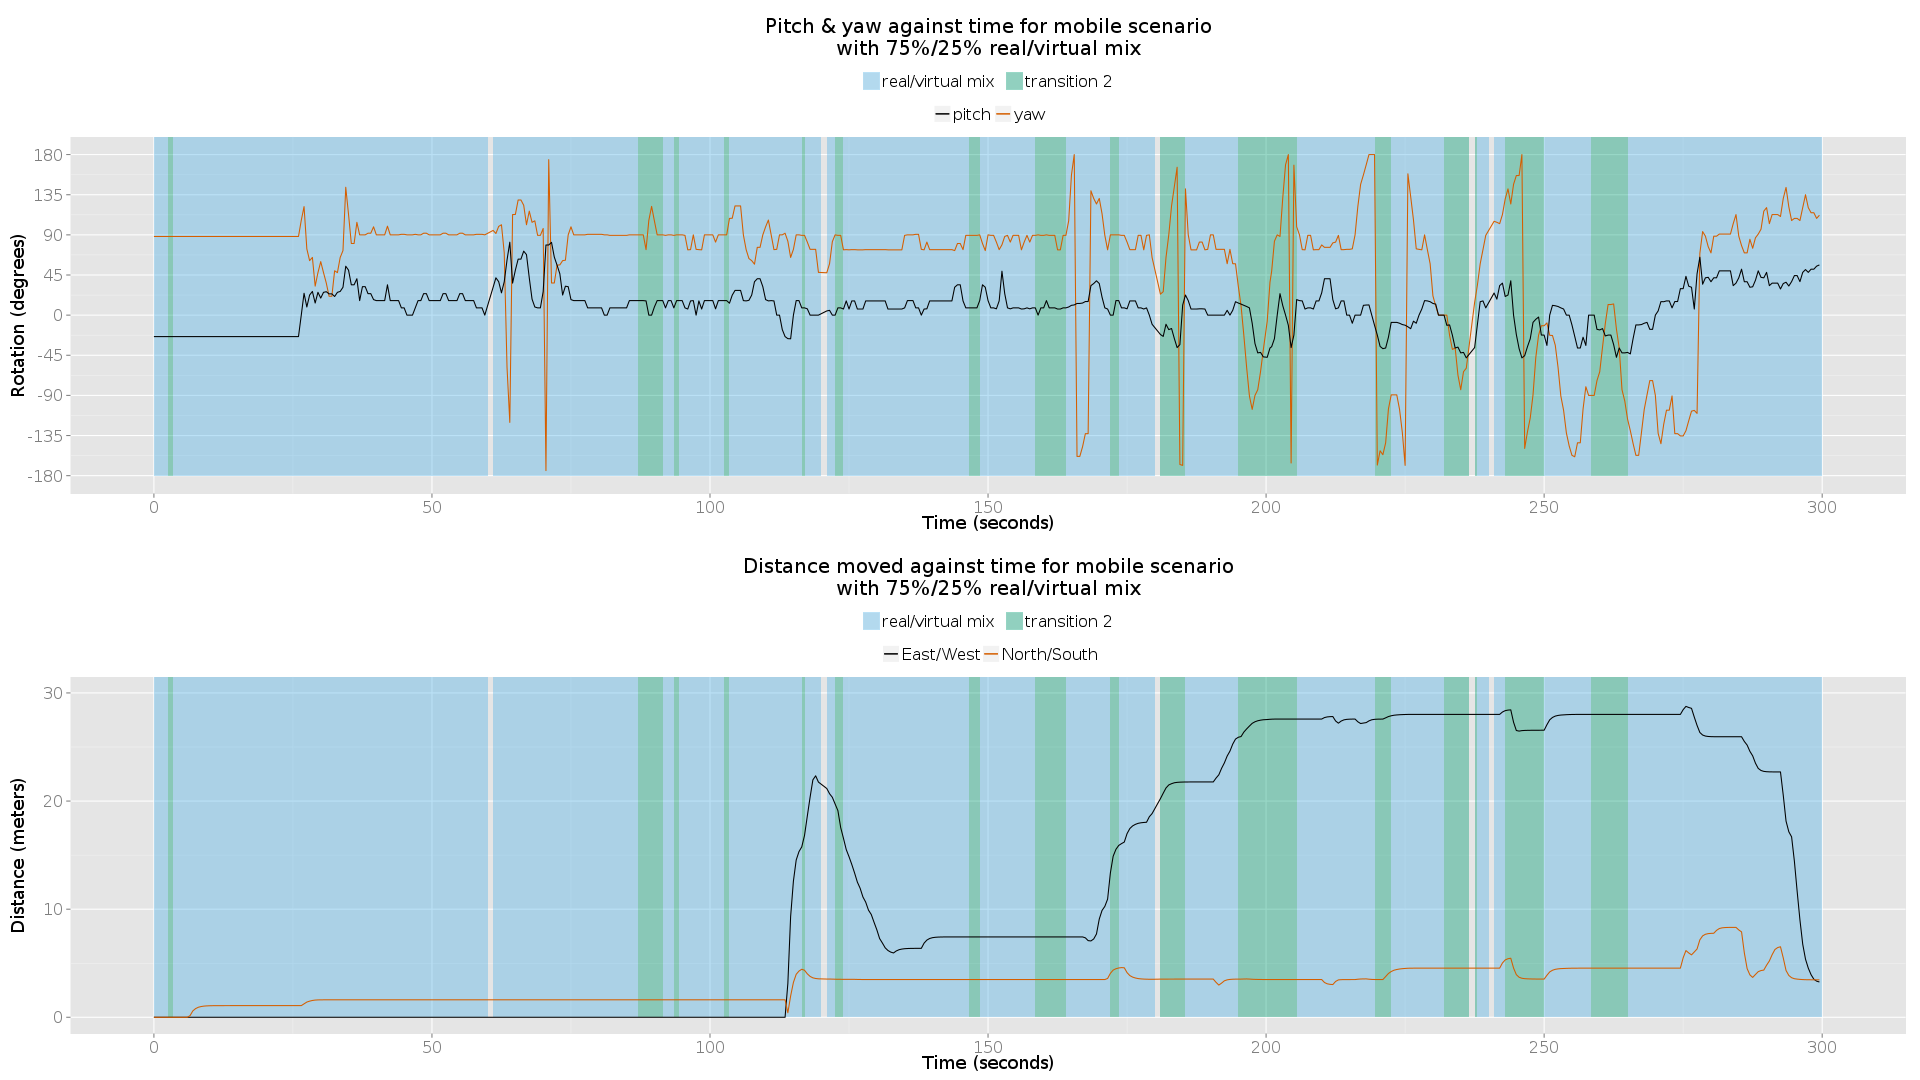
\includegraphics[width=\textwidth]{2.2/15_75_2up.png}
	\caption{Some images, yah.}
	\end{center}
\end{figure}

\clearpage

\begin{figure}[h]
	\begin{center}
	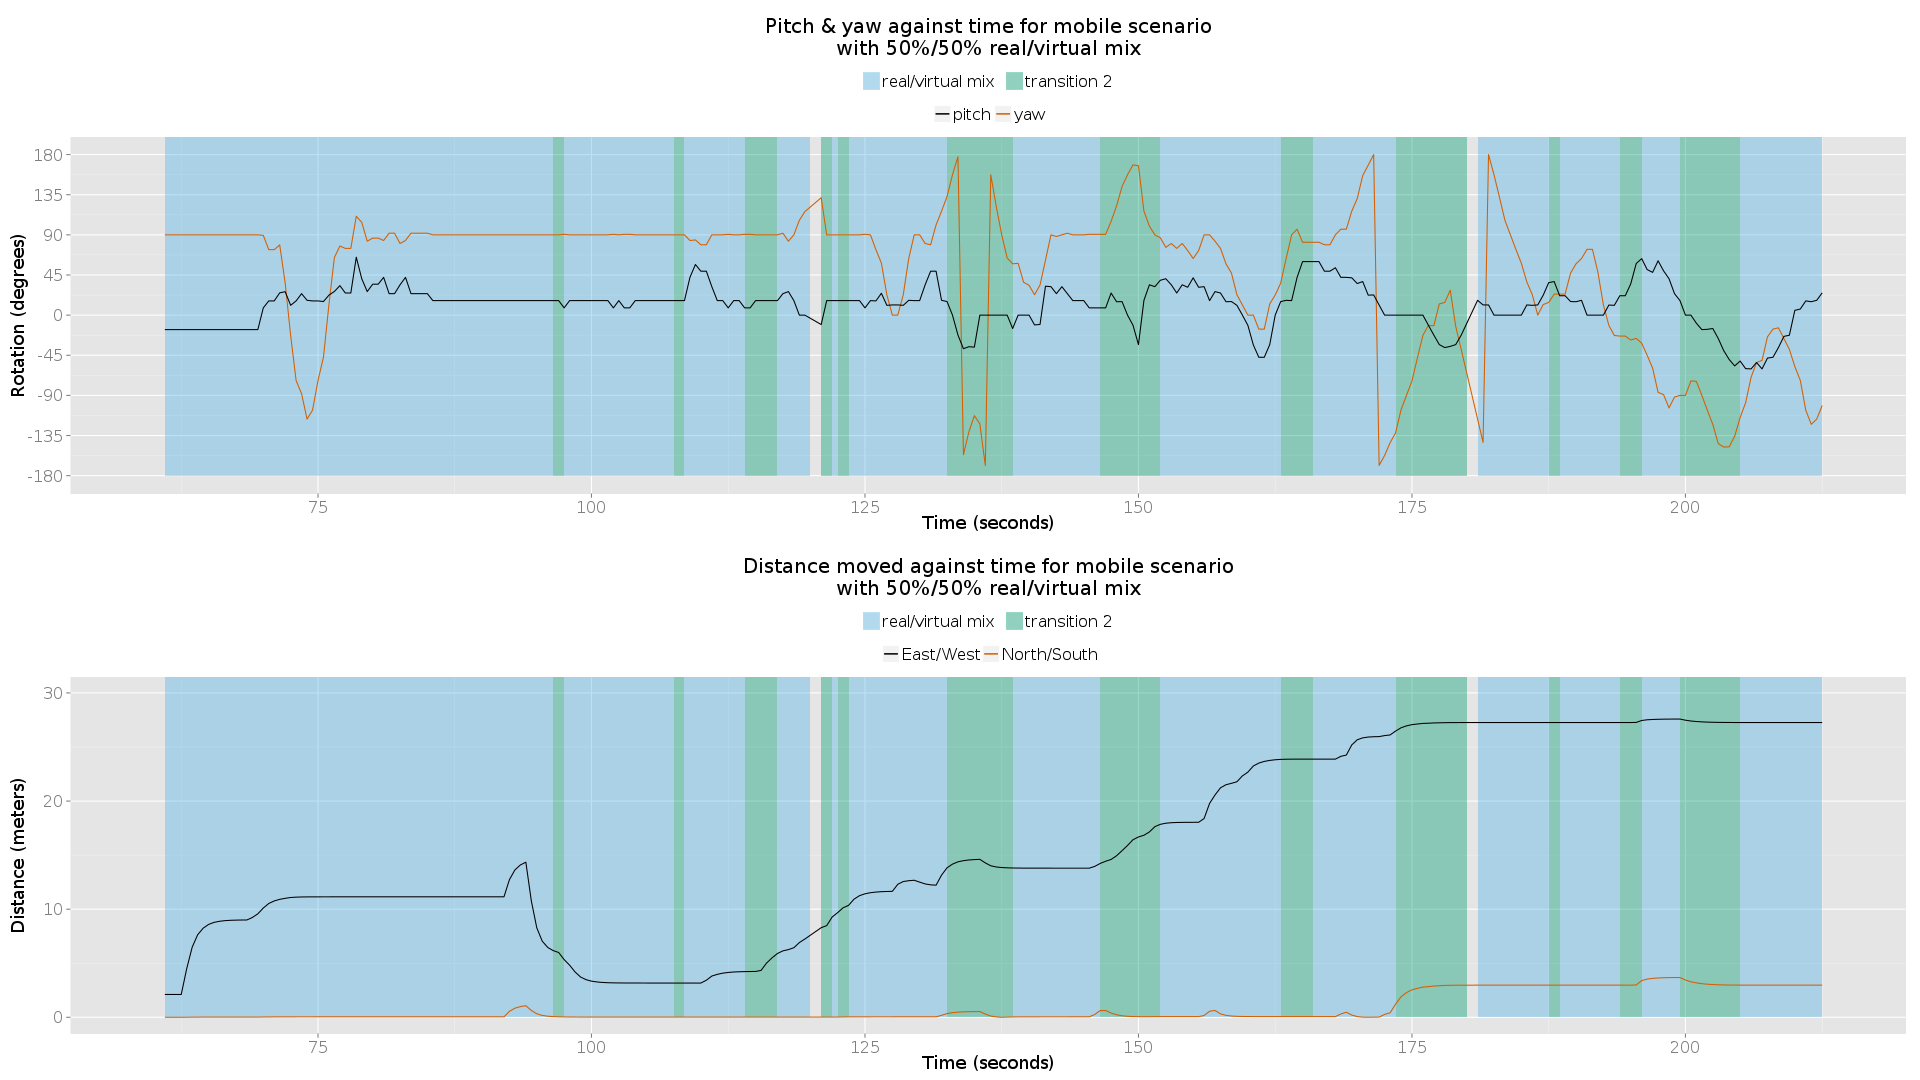
\includegraphics[width=\textwidth]{2.2/15_50_2up.png}
	\caption{Some images, yah.}
	\end{center}
\end{figure}

%=========================================================================================================

\clearpage

\subsection{Participant 16}

\begin{figure}[h]
	\begin{center}
	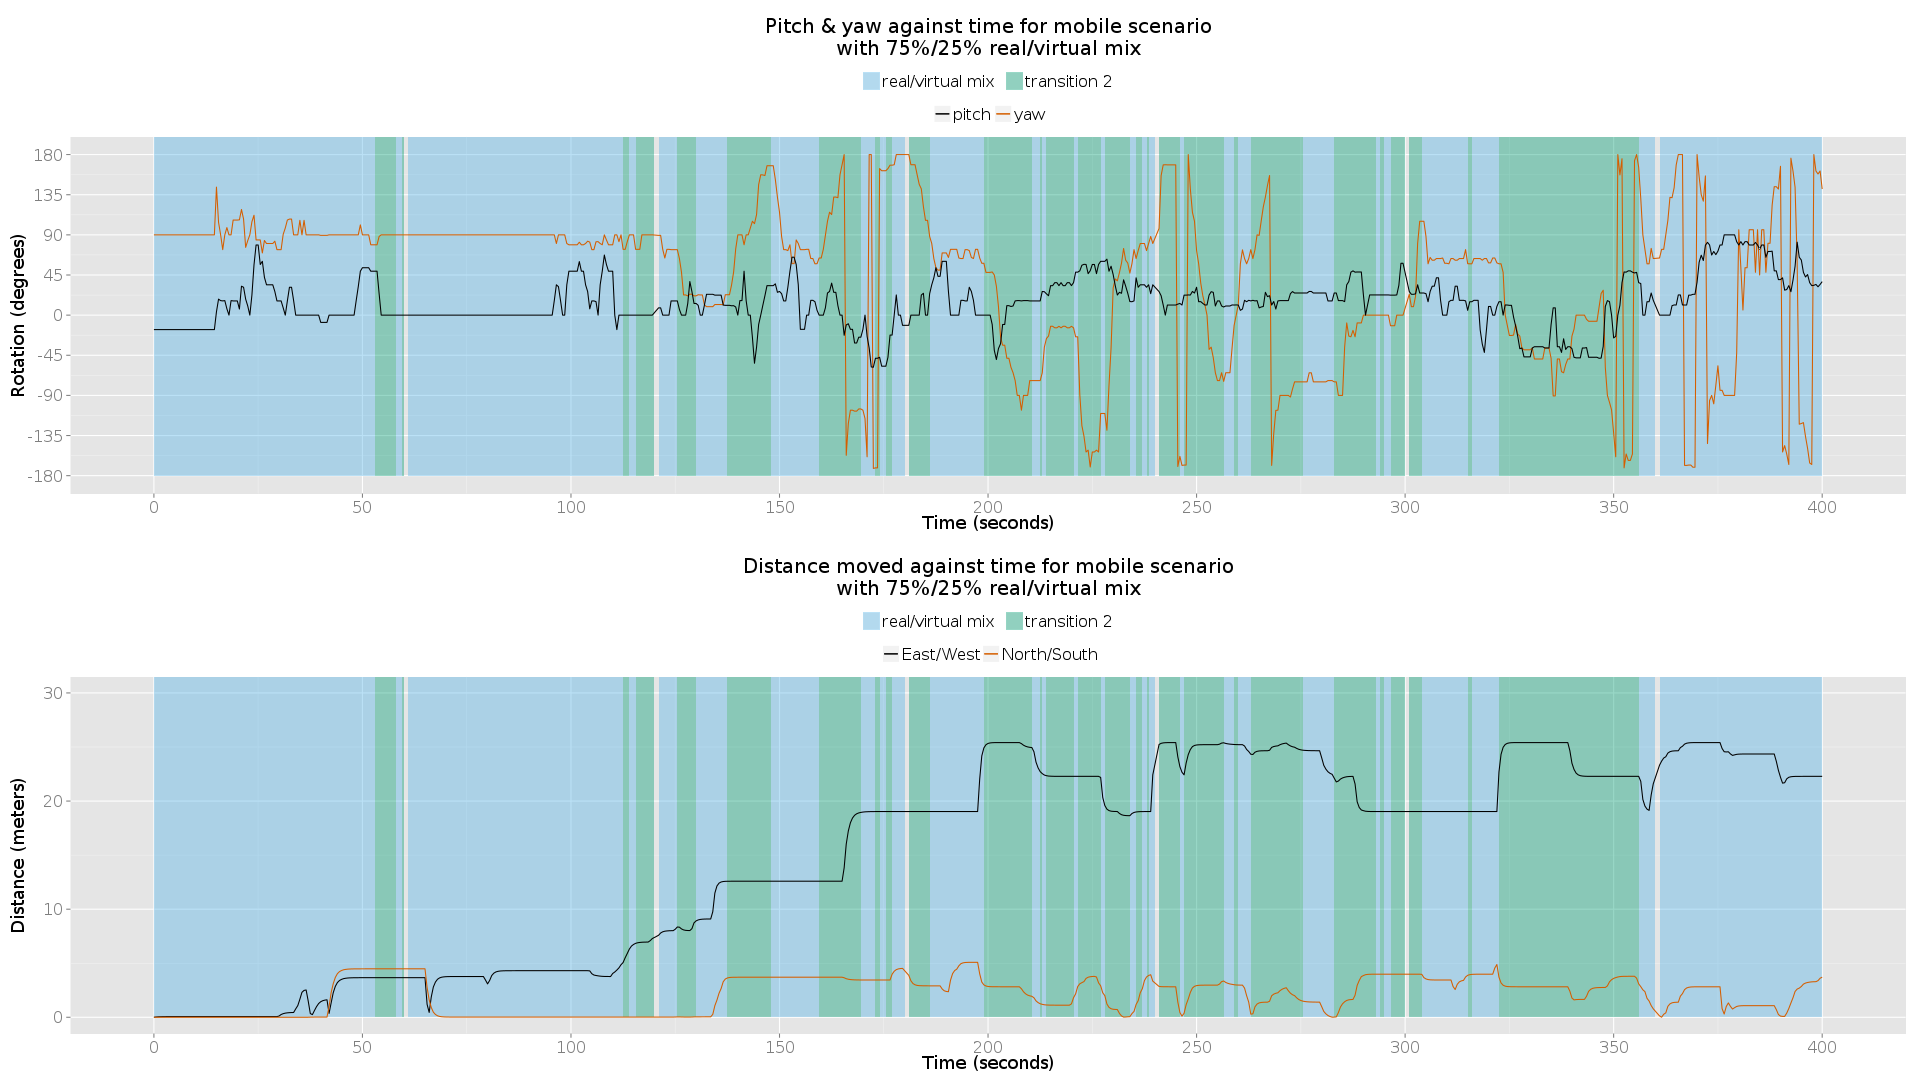
\includegraphics[width=\textwidth]{2.2/16_75_2up.png}
	\caption{Some images, yah.}
	\end{center}
\end{figure}

\clearpage

\begin{figure}[h]
	\begin{center}
	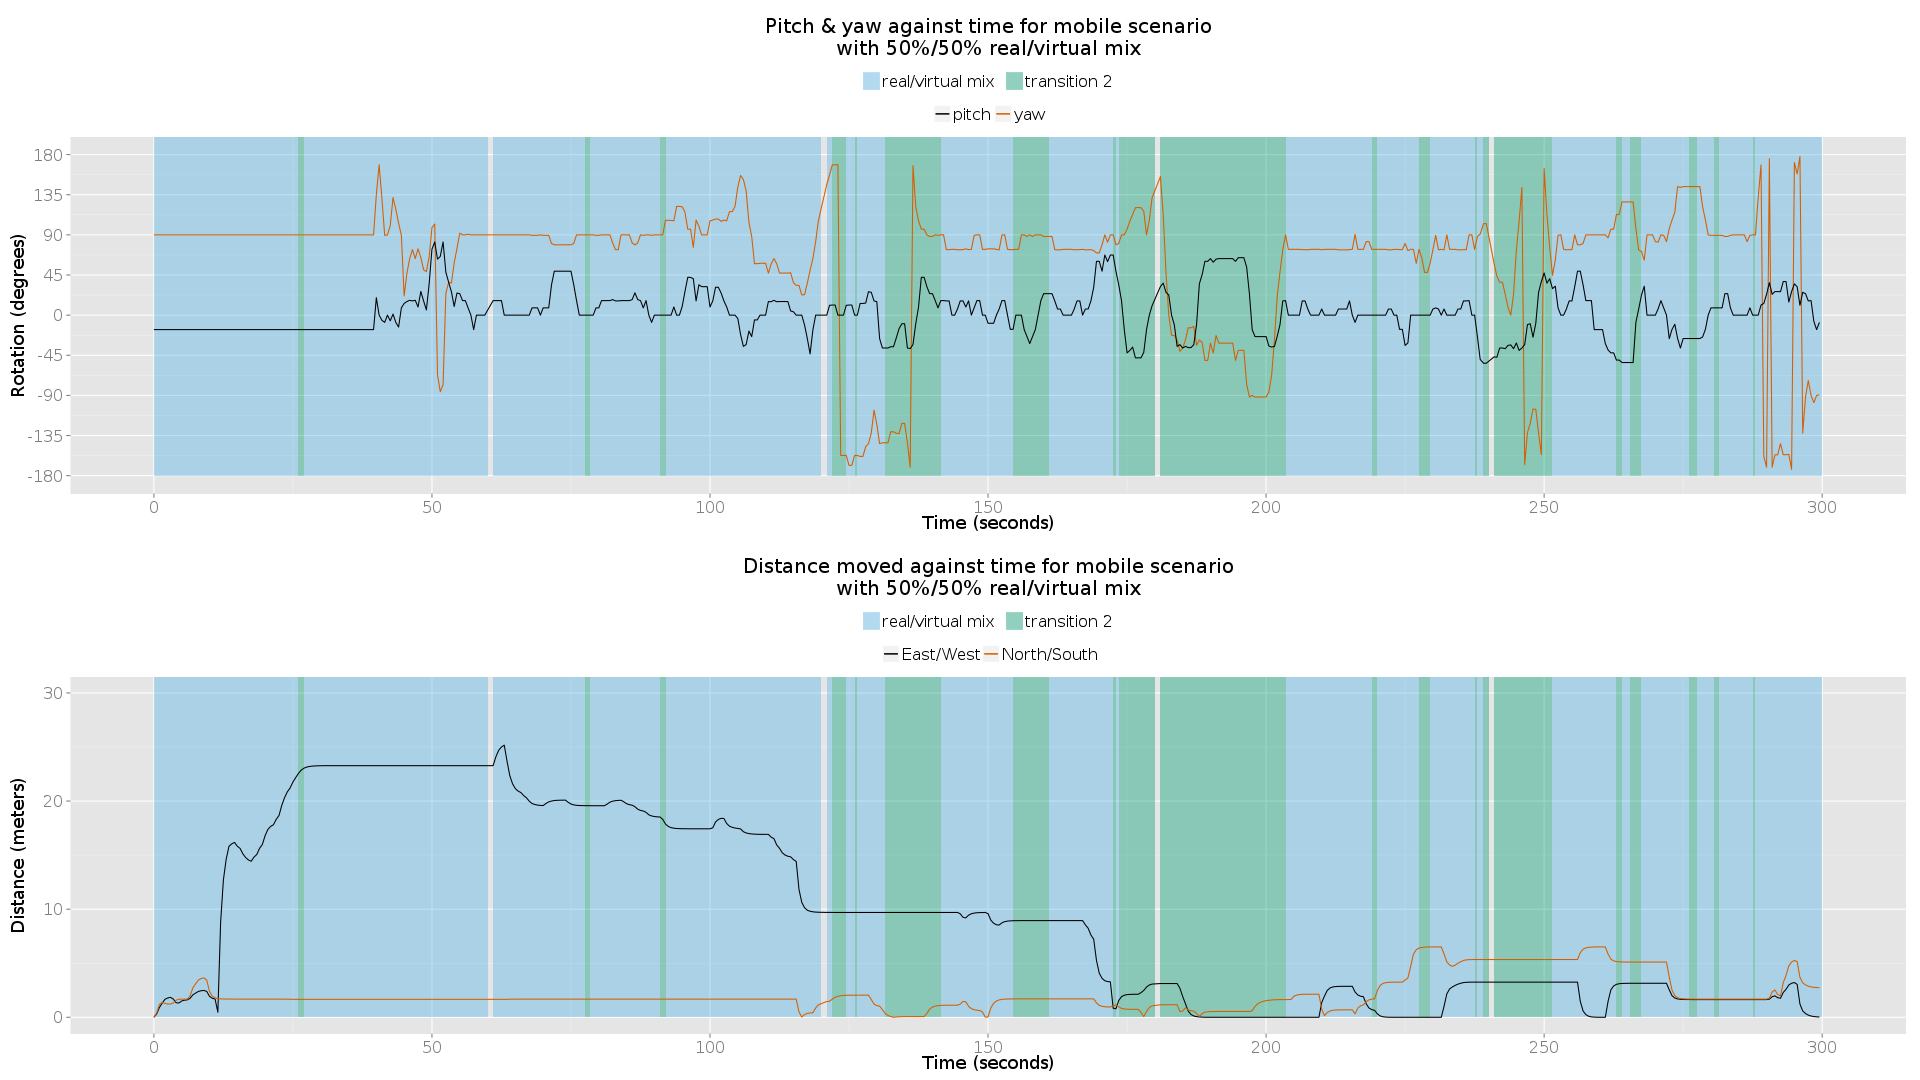
\includegraphics[width=\textwidth]{2.2/16_50_2up.png}
	\caption{Some images, yah.}
	\end{center}
\end{figure}

%=========================================================================================================

\clearpage

\subsection{Participant 17}

\begin{figure}[h]
	\begin{center}
	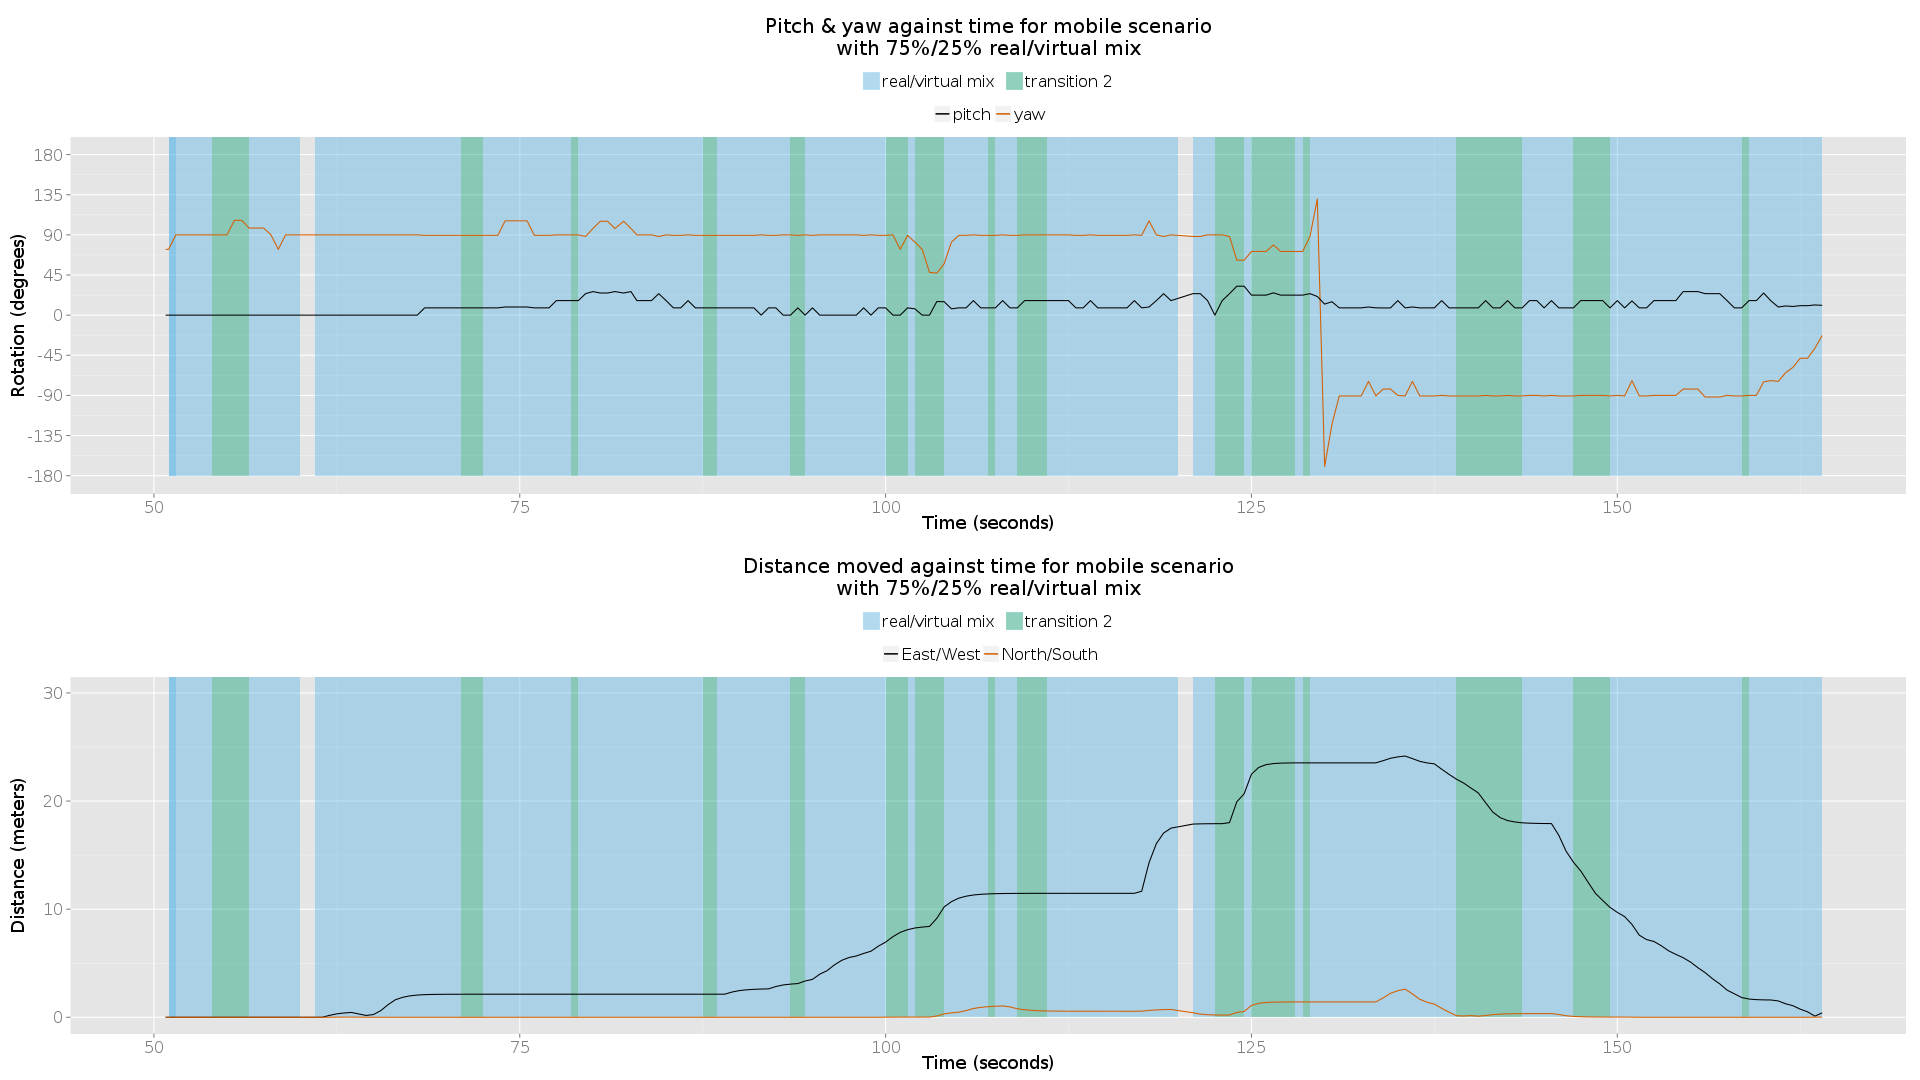
\includegraphics[width=\textwidth]{2.2/17_75_2up.png}
	\caption{Some images, yah.}
	\end{center}
\end{figure}

\clearpage

\begin{figure}[h]
	\begin{center}
	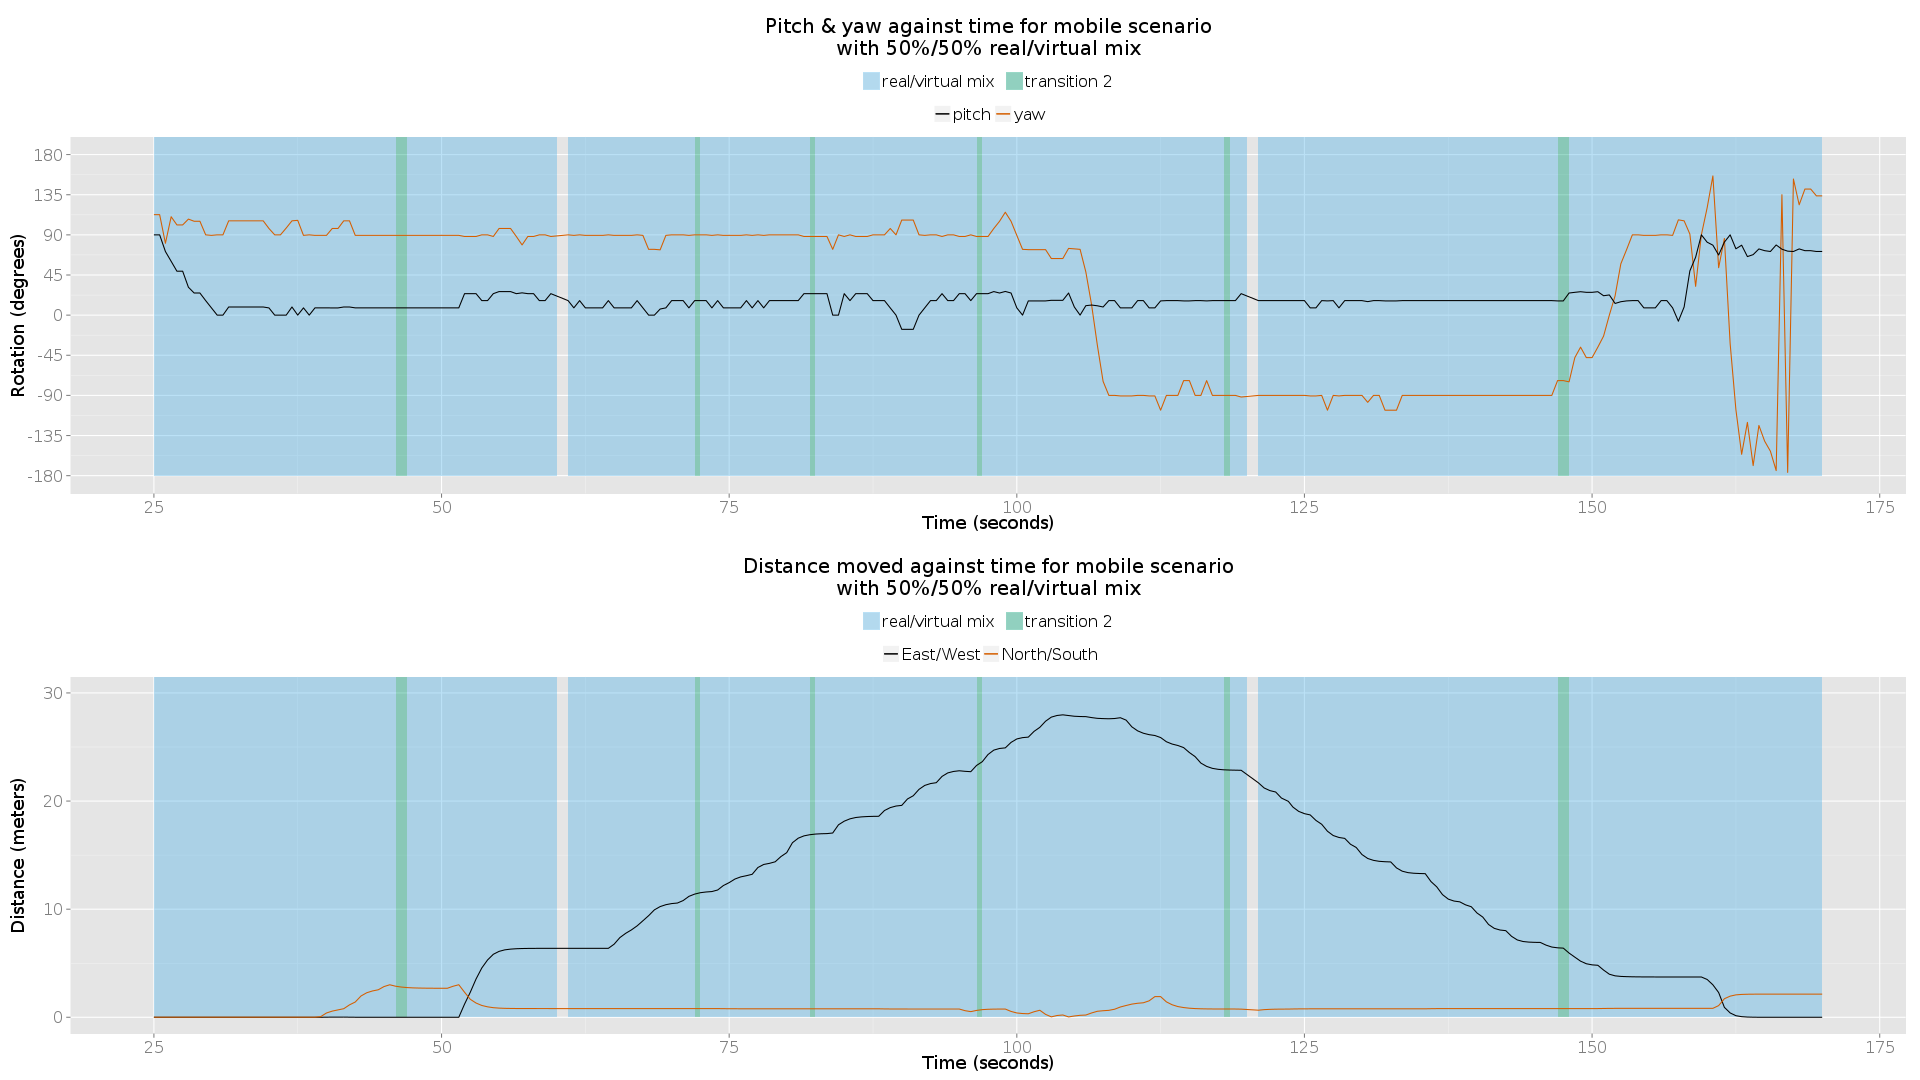
\includegraphics[width=\textwidth]{2.2/17_50_2up.png}
	\caption{Some images, yah.}
	\end{center}
\end{figure}

%=========================================================================================================